%%%%%%%%%%%%%%%%%%%%%%%%%%%%%%%%%%%%%%%%%%%%%%%%%%%%%%%%%%
%   Vorlage von:
%
%   Prof. Dr. Bernhard Drabant
%   Prof. Dr. Dennis Pfisterer
%   Prof. Dr. Julian Reichwald
%
%%%%%%%%%%%%%%%%%%%%%%%%%%%%%%%%%%%%%%%%%%%%%%%%%%%%%%%%%%
%
% Änderungen und Anpassungen von Max Darmstadt
%
%%%%%%%%%%%%%%%%%%%%%%%%%%%%%%%%%%%%%%%%%%%%%%%%%%%%%%%%%%
%	ANLEITUNG: 
%
%   1. Ersetzen Sie firmenlogo.jpg im Verzeichnis img
%   2. Passen Sie alle Stellen im Dokument an, die mit 
%      @stud markiert sind
%
%%%%%%%%%%%%%%%%%%%%%%%%%%%%%%%%%%%%%%%%%%%%%%%%%%%%%%%%%%

%%%%%%%%%%%%%%%%%%%%%%%%%%%%%%%%%%%%%%%%%%%%%%%%%%%%%%%%%%
%	ACHTUNG: 
%
%   Für das Erstellen des Literaturverzeichnisses wird das 
%   modernere Paket biblatex in Kombination mit biber 
%   verwendet -- nicht mehr das ältere BibTex!
%   Bitte stellen Sie ggf. Ihre TeX-Umgebung entsprechend 
%   ein (z.B. TeXStudio: Einstellungen --> Erzeugen --> 
%   Standard Bibliographieprogramm: biber)
%
%%%%%%%%%%%%%%%%%%%%%%%%%%%%%%%%%%%%%%%%%%%%%%%%%%%%%%%%%%

% Layout des Dokumentes festlegen: 12pt = Schriftgröße,Abstand für die Bindung der Arbeit, DIV immer gleichgroß wie die Schrift + Satzspiegelgröße, Für mehr Platz auf der Seite, wahrscheinlich ob man bei der A4 seite auch nach unten mehr Platz hat ,Größe der Beschriftungsfläche,ermöglicht Absätze, Literaturverzeichnis zum Inhaltsverzeichnis , ,irgendwas mit Abblidungensnamen in Abbildungsverzeichnis aufnehmen, toc= TableOfContents ,Nummerierung im Inhaltsverzeichnis ohne Punkt, Maße der Fußlinie aus Plain übernommen
\documentclass[12pt,BCOR=5mm,DIV=12,headinclude=on,footinclude=off,parskip=half,bibliography=totoc,listof=entryprefix,
               toc=listof,pointlessnumbers,plainfootsepline]{scrreprt}

%Edit MaxD If you want to change the margins:
%\usepackage[paper=a4paper,left=30mm,right=30mm,top=25mm,bottom=25mm]{geometry}

% Elementare Pakete, Konfigurationen und Definitionen werden geladen
% !TEX root =  master.tex
%      HYPERREF

%%%%%%%%%%%%%%%%%%%%%%%%%%%%%%%%%%%%%%%%%%%%%%%%%%%%%%%%%%
%	ANLEITUNG: 
%
% Passen Sie alle Stellen im Dokument an, die mit 
% @stud markiert sind
%
% Die untersten packages können die oberen überschreiben, deswegen die wichtigen als letztes
%%%%%%%%%%%%%%%%%%%%%%%%%%%%%%%%%%%%%%%%%%%%%%%%%%%%%%%%%%

\usepackage{makeidx}      			  		% allows index generation, mit \index Wörter zum Stichwort Verzeichnis hinzufügen
\usepackage{listings}						%Format Listings properly , um code in Latex als Box einzufügen
\usepackage{lipsum}   						%Blindtext
\usepackage{graphicx}						% use various graphics formats, um Grafiken einzubinden
\usepackage{placeins}
\usepackage{subfig}
\usepackage[german]{varioref} 				% nicer references \vref
\usepackage{caption}						%better Captions
\usepackage{booktabs} 						%nicer Tabs
\usepackage{array}
\usepackage{chngcntr} 						%zum Neudefinieren von Zählern
\usepackage{fnpct} 							% Correct superscripts ; tauscht Fußnote mit Satzzeichen, wenn die Fußnote vor dem Satzzeichen steht
\usepackage[T1]{fontenc} 					%ermöglicht das Verwenden von Umlauten
\usepackage[utf8]{inputenc}					%Inputcode festlegen
\usepackage{calc}							% Used for extra space below footsepline
\usepackage[printonlyused]{acronym} 		%delete content of the square brackets to force print all acronyms
\usepackage{algorithm}  					% um code in Latex als Box(ähnlich wie eine figure) einzufügen
\usepackage{algpseudocode} 					%für verschiedene darstellweisen des pseudocodes von algorithm
%\usepackage{url} 							% Um urls einzufügen, veraltet, funktion mitlerweile bei hyperref integriert
\usepackage{comment}						%Für Kommentarabschnitte: \begin{comment} \end{comment}
%Edit MaxD %%%%%%%%%%%%%%%%%%%%%%%%%%%%%%%%%%%%%%%%%%%%%%%%%%%%
\usepackage{geometry}						%Zum Verändern der Gestaltung einer Seite: breite, höhe, oberer, unterer Rand, Ausdruck(einseitig, doppelseitig etc)
\usepackage{tikz}							%Zum Darstellen von Grafiken wie:  geometrische Formen oder Koordinatensysteme



\usepackage{tikz}
\usetikzlibrary{calc}
\usetikzlibrary{arrows.meta}
\usetikzlibrary{positioning}
\usetikzlibrary{shapes}
\usetikzlibrary{fit}
\usetikzlibrary{positioning}
\usetikzlibrary{shadows}


\usepackage{footnote}						%Für Fußnoten: \footnote{<text>}
\usepackage{wrapfig}						%Für Schrift umflossene Bilder
\usepackage{float}							%Ermöglicht bei figures: "das bestmögliche platzieren auf der Website"
\usepackage{array,multirow,graphicx}		%array = ermöglicht es, Spalten mit fester Breite auch zentriert oder rechtsbündig auszurichten
											%multirow = ermöglicht in Tabellen, dass Spalten und Zeilen zusammengefasst werden können
											%graphicx = Zum Einbinden von Bildern
\usepackage{listings}						% Um Programmcode in Latex einzubinden: \begin{lstlisting} ; \end{lstlisting}
\lstset{breaklines,numbers=left,xleftmargin=2em,frame=single,framexleftmargin=2em}    % automatische Zeilenumbrüche, wo die line numbers hinsollen, dicke des linken Randes; Rahmen um den Code;  

\usepackage{xargs}%Commands mit mehreren optionalen Parametern möglich
\usepackage[colorinlistoftodos,prependcaption,textsize=tiny]{todonotes} % Todonotes: mit \todo[]{} \missingfigure{} notes für fehlende Elemente einfügen, mit \listoftodos Liste der todos anzeigen lassen
\newcommandx{\unsure}[2][1=]{\todo[linecolor=red,backgroundcolor=red!25,bordercolor=red,#1]{#2}}
\newcommandx{\change}[2][1=]{\todo[linecolor=blue,backgroundcolor=blue!25,bordercolor=blue,#1]{#2}}
\newcommandx{\info}[2][1=]{\todo[linecolor=green,backgroundcolor=green!25,bordercolor=green,#1]{#2}}
\newcommandx{\improvement}[2][1=]{\todo[linecolor=purple,backgroundcolor=purple!25,bordercolor=purple,#1]{#2}}
\newcommandx{\thiswillnotshow}[2][1=]{\todo[disable,#1]{#2}} % usable todo commands: todo, unsure, change, info, improvement, thiswillnotshow

\usepackage[mediumspace,mediumqspace,Grey,squaren]{SIunits}
\usepackage{pgfplots}						%Zum Darstellen von Grafiken, Koodinatensystemen(auch mehrdimensional)
\usepgfplotslibrary{dateplot}				%Bei Grafiken zum Benutzen von Daten
\usepackage{pgfplotstable}					%Zur Tabellennachbearbeitung
\pgfplotsset{compat=1.16}
%\usepackage{draftwatermark}%Delete after you are done with your thesis. This line creates the "Draft" Watermark
\usepackage{setspace}						%Zeilenabstand 3 Optionen: singlespacing; onehalfspacing; doublespacing

%Edit MaxD Fixes line breaks in columns of tables. Example: C{2cm}
\newcolumntype{L}[1]{>{\raggedright\arraybackslash}p{#1}} % left fixed width
\newcolumntype{C}[1]{>{\centering\arraybackslash}p{#1}} % center fixed width
\newcolumntype{R}[1]{>{\raggedleft\arraybackslash}p{#1}} % flush right fixed width
%%%%%%%%%%%%%%%%%%%%%%%%%%%%%%%%%%%%%%%%%%%%%%%%%%%%%%%%%%%%%%%%%%%%%

%originally in line 21 needed to be moved to the end
\usepackage[hidelinks=true]{hyperref} % keine roten Markierungen bei Links

%
% @stud
%
%	FONT SELECTION: Entweder 1) Latin Modern oder 2) Times / Helvetica ( FONT = Schriftart)
\usepackage{lmodern}             % 1) Latin modern font
%\usepackage{mathptmx}           % 2) Helvetica / Times New Roman fonts (2 lines)
%\usepackage[scaled=.92]{helvet} % 2) Helvetica / Times New Roman fonts (2 lines)

%
% @stud
%
%	LANGUAGE SETTINGS
\usepackage[ngerman]{babel} 	        % german language
\usepackage[german=quotes]{csquotes} 	% correct quoting using \enquote{}
%\usepackage[english]{babel}          % english language
%\usepackage{csquotes} 	              % correct quoting using \enquote{}

%
% @stud
%
% Uncomment the following lines to support hard URL breaks in bibliography 
%\apptocmd{\UrlBreaks}{\do\f\do\m}{}{}
%\setcounter{biburllcpenalty}{9000}% Kleinbuchstaben
%\setcounter{biburlucpenalty}{9000}% Großbuchstaben

%
% @stud
%
%	FOOTNOTES: Count footnotes over chapters
\counterwithout{footnote}{chapter}

%	ACRONYMS
\makeatletter
\@ifpackagelater{acronym}{2015/03/20}
{\renewcommand*{\aclabelfont}[1]{\textbf{{\acsfont{#1}}}}}{}
\makeatother

%	LISTINGS
\renewcommand{\lstlistingname}{Quelltext} 
\renewcommand{\lstlistlistingname}{Quelltextverzeichnis}
\lstset{numbers=left,
	numberstyle=\tiny,
	captionpos=b,
	basicstyle=\ttfamily\small}

%	ALGORITHMS
\renewcommand{\listalgorithmname}{Algorithmenverzeichnis }
\floatname{algorithm}{Algorithmus}

%		PAGE HEADER / FOOTER
%	    Warning: There are some redefinitions throughout the master.tex-file!  DON'T CHANGE THESE REDEFINITIONS!
\RequirePackage[automark,headsepline,footsepline]{scrlayer-scrpage}
\pagestyle{scrheadings}
%\renewcommand*{\pnumfont}{\upshape\sffamily}
%\renewcommand*{\headfont}{\upshape\sffamily}
%\renewcommand*{\footfont}{\upshape\sffamily}
\renewcommand{\chaptermarkformat}{}
\RedeclareSectionCommand[beforeskip=0pt]{chapter}
\clearscrheadfoot

\ifoot[\rule{0pt}{\ht\strutbox+\dp\strutbox}DHBW Mannheim]{\rule{0pt}{\ht\strutbox+\dp\strutbox}DHBW Mannheim}
\ofoot[\rule{0pt}{\ht\strutbox+\dp\strutbox}\pagemark]{\rule{0pt}{\ht\strutbox+\dp\strutbox}\pagemark}
\ohead{\headmark}

\newcommand{\TitelDerArbeit}[1]{\def\DerTitelDerArbeit{#1}\hypersetup{pdftitle={#1}}}
\newcommand{\AutorDerArbeit}[1]{\def\DerAutorDerArbeit{#1}\hypersetup{pdfauthor={#1}}}
\newcommand{\Firma}[1]{\def\DerNameDerFirma{#1}}
\newcommand{\Kurs}[1]{\def\DieKursbezeichnung{#1}}
\newcommand{\Abteilung}[1]{\def\DerNameDerAbteilung{#1}}
\newcommand{\Studiengangsleiter}[1]{\def\DerStudiengangsleiter{#1}}
\newcommand{\WissBetreuer}[1]{\def\DerWissBetreuer{#1}}
\newcommand{\FirmenBetreuer}[1]{\def\DerFirmenBetreuer{#1}}
\newcommand{\Bearbeitungszeitraum}[1]{\def\DerBearbeitungszeitraum{#1}}
\newcommand{\Abgabedatum}[1]{\def\DasAbgabedatum{#1}}
\newcommand{\Matrikelnummer}[1]{\def\DieMatrikelnummer{#1}}
\newcommand{\Studienrichtung}[1]{\def\DieStudienrichtung{#1}}
\newcommand{\ArtDerArbeit}[1]{\def\DieArtDerArbeit{#1}}
\newcommand{\Literaturverzeichnis}{Literaturverzeichnis}

\newcommand{\settingBibFootnoteCite}{
	\setlength{\bibparsep}{\parskip}		  % Add some space between biblatex entries in the bibliography
	\addbibresource{bibliography.bib}	    % Add file bibliography.bib as biblatex resource
	\DefineBibliographyStrings{ngerman}{andothers = {{et\,al\adddot}},}
	%Following two lines commented, because those features are no longer supported
	%\AdaptNoteOpt\footcite\multfootcite   % Will add  separators if footcite is called multiple consecutive times 
	%\AdaptNoteOpt\autocite\multautocite   % Will add  separators if autocite is called multiple consecutive times
}

\newcommand{\setTitlepage}{
	% !TEX root =  master.tex
\begin{titlepage}
\begin{minipage}{\textwidth}
		\vspace{-2cm}
		\noindent 
\includegraphics[scale=0.25]{\imagedir/firmenlogo.jpg} \hfill 
\includegraphics{\imagedir/logo.jpg}
\end{minipage}
\vspace{1em}
%\sffamily
\begin{center}
	{\textsf{\large Duale Hochschule Baden-W\"urttemberg Mannheim}}\\[4em]
	{\textsf{\textbf{\large{\DieArtDerArbeit}arbeit}}}\\[6mm]
	{\textsf{\textbf{\Large{}\DerTitelDerArbeit}}} \\[6mm]%[1.5cm]
	%{\textsf{\large{}Eine vergleichende Untersuchung und Konzeption}}\\[1.5cm]
	{\textsf{\textbf{\large{}Studiengang Wirtschaftsinformatik}}\\[6mm]
	\textsf{\textbf{Studienrichtung \DieStudienrichtung}}}\vspace{7em}
	
	\begin{minipage}{\textwidth}
		\begin{tabbing}
		Wissenschaftliche(r) Betreuer(in): \hspace{0.85cm}\=\kill
		Verfasser(in): \> \DerAutorDerArbeit \\[1.5mm]
		Matrikelnummer: \> \DieMatrikelnummer \\[1.5mm]
		Firma: \> \DerNameDerFirma  \\[1.5mm]
		Abteilung: \> \DerNameDerAbteilung \\[1.5mm]
		Kurs: \> \DieKursbezeichnung \\[1.5mm]
		Studiengangsleiter: \> \DerStudiengangsleiter \\[1.5mm]
		Wissenschaftliche(r) Betreuer(in): \> \DerWissBetreuer \\[1.5mm]
		%\> 0621 4105 1218 \\[1.5mm]
		%\> hans-peter.engel@dhbw-mannheim.de \\[1.5mm]
		Firmenbetreuer(in): \> \DerFirmenBetreuer \\[1.5mm]
		%\> +49 6227 7-70239 \\[1.5mm]
		%\> pierre.grosse@sap.com \\[1.5mm]
		Bearbeitungszeitraum: \> \DerBearbeitungszeitraum\\[1.5mm]
%		alternativ:\\[1.5mm]
		Eingereicht: \> \DasAbgabedatum	
		\end{tabbing}
	\end{minipage}
\end{center}
\end{titlepage}
	\pagenumbering{roman} % Römische Seitennummerierung
	\normalfont	
}

%
% @stud
%
\newcommand{\settingLists}{
	%	Inhaltsverzeichnis
	%\begin{spacing}{0.95} %Change line spacing to fit table of contents on one page
		\tableofcontents
	%\end{spacing}

	%	Abbildungsverzeichnis
	\listoffigures
	%	Tabellenverzeichnis
	%\listoftables
	%	Listingsverzeichnis / Quelltextverzeichnis
	%\lstlistoflistings
	% Algorithmenverzeichnis
	%\listofalgorithms
}

\newcommand{\initializeText}{
	\clearpage
	\ihead{\chaptername~\thechapter} % Neue Header-Definition
	\pagenumbering{arabic}           % Arabische Seitenzahlen
	\onehalfspacing
}

\newcommand{\initializeBibliography}{
	\ihead{}
	\printbibliography[title=Quellenverzeichnis]
	\pagebreak 
	\pagenumbering{roman}
	\cleardoublepage
	\singlespacing
	
	
}

\newcommand{\initializeAppendix}{
	\appendix
	\ihead{\appendixname~\thechapter}
	\ihead{}
	\singlespacing
	
}

%EditMaxD
\newcommand{\setTodo}{
	\listoftodos[Todos]
	\newpage
}

%Defining Custom Colors
\definecolor{sapBlue1}{RGB}{0,185,242}
\definecolor{sapBlue2}{RGB}{1,156,224}
\definecolor{sapBlue3}{RGB}{12,126,207}
\definecolor{sapBlue4}{RGB}{22,97,190}

\definecolor{sapGold}{RGB}{240,171,0}


%%%%%%%%%%%%%%%%%%%%%%%%%%%%
%
% @stud
%
%	SCHRIFTART (Schrift mit oder ohne Serifen im gesamten Text) 
%
% mit Serifen
%\addtokomafont{disposition}{\rmfamily}
%\renewcommand*{\familydefault}{\rmdefault}
%
% ohne Serifen (default)
%\addtokomafont{disposition}{\sffamily}
%
%%%%%%%%%%%%%%%%%%%%%%%%%%%%

%%%%%%%%%%%%%%%%%%%%%%%%%%%%
%
% @stud
%
% PERSÖNLICHE ANGABEN (BITTE VOLLSTÄNDIG EINGEBEN zwischen den Klammern: {...})
%
\ArtDerArbeit{Projekt} % "Bachelor" oder "Projekt" wählen
\TitelDerArbeit{Evaluierung und Implementierung einer neuen Suchoberfläche für das SAP Product Lifecycle Management im S/4HANA Umfeld}
\AutorDerArbeit{Jonas Mayer}
\Abteilung{AIS PLM}
\Firma{SAP SE}
\Kurs{WWI20SCB}
\Studienrichtung{Sales \& Consulting}
\Matrikelnummer{7415525}
\Studiengangsleiter{Herr Prof. Dr. -Ing. Martin}
\WissBetreuer{Stefanie Bell}
\FirmenBetreuer{Marco Armbruster}
\Bearbeitungszeitraum{02.08.2021 -- 22.11.2021}
\Abgabedatum{22.11.2021}
%
%%%%%%%%%%%%%%%%%%%%%%%%%%%%

%%%%%%%%%%%%%%%%%%%%%%%%%%%%
%
% @stud
%
%	BIBLIOGRAPHY (@stud: Bibliographie-Stil wählen - Position und Indizierung)
%
% Auswahl zwischen: IEEE Style, ALPHABETIC Style, HARVARD Style, AUTHOR-YEAR Style 
%
% (oder eigenen zulässigen Stil wählen) 
%

% Position des Zitats
%
%\newcommand{\position}{inline} 
\newcommand{\position}{footnote}

% Indizierung des Zitats
%
% 1) NUMERIC Style - e. g. [12]
%\newcommand{\indextype}{numeric} 
%
% 2) ALPHABETIC Style - e. g. [AB12]
%\newcommand{\indextype}{alphabetic} 
%
% 3) IEEE Style - numeric kind of style 
%\newcommand{\indextype}{ieee} 
%
% 4) HARVARD Style 
%\newcommand{\indextype}{apa} 
%
% 5) CHICAGO Style 
\newcommand{\indextype}{authoryear}
%
%%%%%%%%%%%%%%%%%%%%%%%%%%%%
%Edit MaxD commented the line below, because it made the font look weird.
%\renewcommand*{\familydefault}{\sfdefault}

\usepackage[backend=biber, autocite=\position, style=\indextype]{biblatex} 	%package zur Gestaltung des Literaturverzeichnisses:Legt das Backend zum Sortieren der Bibliographie fest, mit sorting=ynt lässt sich festlegen wie das Literaturverzeichnis sortiert werden soll, lässt sich bibliography style festlegen: style=alphabetic
\apptocmd{\UrlBreaks}{\do\f\do\m}{}{}
\setcounter{biburllcpenalty}{9000}% Kleinbuchstaben
\setcounter{biburlucpenalty}{9000}% Großbuchstaben

\settingBibFootnoteCite

\newcommand{\abs}{\par\vskip 0.2cm\goodbreak\noindent}
\newcommand{\nl}{\par\noindent}
\newcommand{\mcl}[1]{\mathcal{#1}}
\newcommand{\nowrite}[1]{}
\newcommand{\NN}{{\mathbb N}}

\newcommand{\imagedir}{img}

\makeindex %erstellt die Indexdatei, in die dann mit \index{Stichwort} aus dem Main Einträge gemacht werden können
\begin{document}
%\setTodo
\setTitlepage

%%%%%%%%%%%%%%%%%%%%%%%%%%%%%%%%%%%%%%%%%%%%%%%%%%%%%%%%%%%%%%%%%%%%%%%%%%%%%%%%%%%%%%%%%%
% KAPITEL UND ANHÄNGE
%
% @stud:
%   - nicht benötigte: auskommentieren/löschen
%   - neue: bei Bedarf hinzufügen mittels input-Kommando an entsprechender Stelle einfügen
%%%%%%%%%%%%%%%%%%%%%%%%%%%%%%%%%%%%%%%%%%%%%%%%%%%%%%%%%%%%%%%%%%%%%%%%%%%%%%%%%%%%%%%%%%

%%%%%%%%%%%%%%%%%%%%%%%%%%%%%%%%%%%
% SPERRVERMERK
%
% @stud: nondisclosurenotice.tex bearbeiten
%
%\input{nondisclosurenotice} 
%%%%%%%%%%%%%%%%%%%%%%%%%%%%%%%%%%%

%%%%%%%%%%%%%%%%%%%%%%%%%%%%%%%%%%%
%	KURZFASSUNG
%
% @stud: acknowledge.tex bearbeiten
%
%\input{acknowledge} 
%%%%%%%%%%%%%%%%%%%%%%%%%%%%%%%%%%%

%%%%%%%%%%%%%%%%%%%%%%%%%%%%%%%%%%%
%	Disclaimer
%
% @stud: acknowledge.tex bearbeiten
%
% Für Gender und englische Begriffe: 
\chapter*{Disclaimer}

In dieser Arbeit wird aus Gründen der besseren Lesbarkeit das generische Maskulinum verwendet. Weibliche und anderweitige Geschlechteridentitäten werden dabei ausdrücklich mitgemeint, soweit es für die Aussage erforderlich ist. Des Weiteren werden die englischen Begriffe der Informationstechnologie in ihrer Originalsprache verwendet, um die Bedeutung der Ausdrücke nicht zu verfälschen.
\pagebreak 
%%%%%%%%%%%%%%%%%%%%%%%%%%%%%%%%%%%

%%%%%%%%%%%%%%%%%%%%%%%%%%%%%%%%%%%
%	KURZFASSUNG
%
% @stud: abstract.tex bearbeiten
%
% !TEX root =  master.tex
%\newgeometry{top=30mm,bottom=40mm}
%\thispagestyle{empty}
\thispagestyle{plain}
\begin{minipage}{\textwidth}
        \vspace{-3.5cm}
        \noindent  \hfill 
\includegraphics{\imagedir/logo.jpg}
    \end{minipage}
\begin{flushright}
        \vspace{-1cm}
        \footnotesize{Wirtschaftsinformatik}\\
        \medskip
        \small{\textbf{\DerTitelDerArbeit}}\\
        \medskip
        \footnotesize{{\DieArtDerArbeit}arbeit}\\
        \footnotesize{\DerAutorDerArbeit}\\
        \footnotesize{\DerNameDerFirma}\\
\end{flushright}
\vspace{-1cm}
\section*{Kurzfassung}
%\vspace{-0.3cm}

%\textbf{Kurzfassung}\\\\

\improvement{Vergangenheitsform???}

Die Kfz-Versicherungsbranche befindet sich im Zuge der digitalen Transformation in einem enormen Wandel. So erwarten die Versicherungsnehmer heutzutage einen komfortablen und reibungslosen Online-Service. Um wettbewerbsfähig zu bleiben, müssen Kfz-Versicherer deshalb mithilfe einer digitalen Plattform ihre Prozesse optimieren, „sich mit Partnern integrieren“ und zusätzliche Services für den Endkunden anbieten. Die SAP Business Technology Platform (BTP) ist eine dazu passende Lösung, mit der Unternehmen die digitale Transformation meistern können. Ziel der vorliegenden Abhandlung ist es daher, die Anforderungen der Kfz-Versicherer an eine digitale Plattform zu identifizieren, um anschließend beurteilen zu können, inwiefern diese Anforderungen von der SAP Business Technology Platform erfüllt werden.\\
Zur Beantwortung der Forschungsfrage wurde die Task-Technology-Fit-Theorie angewendet. Dabei wurden zunächst die Anforderungen der Kfz-Versicherer durch eine systematischen Literaturanalyse identifiziert und anschließend mittels Experteninterviews ergänzt und evaluiert. Die Priorisierung der Experten hat gezeigt, dass bei Erfüllung der grundlegenden Anforderungen, wie Datensicherheit und Skalierbarkeit, für Kfz-Versicherer in den nächsten Jahren vor allem die Anforderungsbereiche Integration und Anwendungsentwicklung wichtig sind. Nach der Identifikation wurden die Anforderungen mit den Technologie-Charakteristika der SAP BTP gegenübergestellt. Hier hat die Analyse gezeigt, dass die SAP BTP 19 der 20 Anforderungen grundlegend erfüllt und damit als digitale Plattform für Kfz-Versicherer gut geeignet ist. Abschließend wurde in der Handlungsempfehlung eine schrittweise Vorgehensweise zur Verwendung der SAP Business Technology Plattform bei Kfz-Versicherern aus dem Analyseergebnis und der Priorisierung der Anforderungen durch die Experten abgeleitet.\\
In weiterführenden Fragestellungen könnte unter anderem erörtert werden, wie sich der Trend der digitalen Ökosysteme auf die Kfz-Versicherungsbranche auswirkt und welche Rolle dabei insbesondere die in dieser Arbeit untersuchten digitalen Plattformen spielen.\\
Die vorliegende Arbeit ist für all jene relevant, die sich mit der digitalen Transformation der deutschen Kfz-Versicherungsbranche befassen, da die Verwendung von digitalen Plattformen ein wichtiger Faktor für den zukünftigen Geschäftserfolg ist.




% Inhalte:
% -Problemstellung
% -Forschungsfrage
% -Methodik
% -Wichtige Ergebnisse
% -Interpretation
% -meist ungefähr 150 Wörter



%\restoregeometry 
%%%%%%%%%%%%%%%%%%%%%%%%%%%%%%%%%%%

%%%%%%%%%%%%%%%%%%%%%%%%%%%%%%%%%%%
% VERZEICHNISSE
%
% @stud: ggf. nicht benötigte Verzeichnisse auskommentieren/löschen in Def. von \settingLists in config.tex
%
\settingLists
%%%%%%%%%%%%%%%%%%%%%%%%%%%%%%%%%%%

%%%%%%%%%%%%%%%%%%%%%%%%%%%%%%%%%%%
% ABKÜRZUNGSVERZEICHNIS
%
% @stud: acronyms.tex bearbeiten
%
% !TEX root =  master.tex
\clearpage
\chapter*{Abkürzungsverzeichnis}	
\addcontentsline{toc}{chapter}{Abkürzungsverzeichnis}

\improvement{Zeilenabstand größer}

\begin{acronym}[XXXXXXX]
	\acro{abap}[ABAP]{Advanced Business Application Programming}
	\acro{ai}[AI]{Artificial Intelligence}
	\acro{apaas}[APaaS]{Application Platform-as-a-Service}
	\acro{api}[API]{Application Programming Interface}
	\acroplural{api}[APIs]{Application Programming Interfaces}	
	\acro{are}[ARE]{Application Runtime Environment}
	\acro{bafin}[BaFin]{Bundesanstalt für Finanzdienstleistungsaufsicht}
	\acro{bi}[BI]{Business Intelligence}
	\acro{btp}[BTP]{Business Technology Platform}
	%\acro{bwa}[BWA]{Business Warehouse Accelerator}
	\acro{cap}[CAP]{Cloud Application Programming}
	\acro{dhbw}[DHBW]{Duale Hochschule Baden-Württemberg}
	\acro{dsgvo}[DSGVO]{Datenschutzgrundverordnung}
	\acro{ebsco}[EBSCO]{Elton B. Stephens Company}
	\acro{erp}[ERP]{Enterprise-Resource-Planning}
	\acro{etl}[ETL]{Extract-Transform-Load}
	\acro{exp}[EXP]{Experte}
	\acro{frida}[FRIDA]{Free Insurance Data Initiative}
	%\acro{es}[ES]{Enterprise Search}
	\acro{gafa}[GAFA]{Google, Apple, Facebook und Amazon}
	\acro{hana}[HANA]{High-performance ANalytic Appliance}
	\acro{hdi}[HDI]{Haftpflichtverband der Deutschen Industrie}
	\acro{http}[HTTP]{Hypertext Transfer Protocol}
	\acro{iaas}[IaaS]{Infrastructure-as-a-Service}
	\acro{ide}[IDE]{Integrated Development Environment}
	\acro{iec}[IEC]{International Electrotechnical Commission}
	\acro{iese}[IESE]{Institut für Experimentelles Software Engineering}
	\acro{iot}[IoT]{Internet-of-Things}
	\acro{iso}[ISO]{International Organization for Standardization}
	\acro{isv}[ISV]{Independent Service Provider}
	\acro{it}[IT]{Informationstechnologie}
	\acro{jstor}[JSTOR]{Journal STORage}
	\acro{ki}[KI]{Künstliche Intelligenz}
	\acro{kfz}[Kfz]{Kraftfahrzeug}
	\acro{ml}[ML]{Machine Learning}
	\acro{nist}[NIST]{National Institute of Standards and Technology}
	\acro{nlp}[NLP]{Neuro-Linguistisches Programmieren}
	\acro{odata}[OData]{Open Data Protocol}
	%\acro{otr}[OTR]{Online Text Repository}
	%\acro{pam}[PAM]{Product Availibility Matrix}
	\acro{paas}[PaaS]{Platform-as-a-Service}
	\acro{psd2}[PSD2]{Payment Services Directive 2}
%	\acro{plm}[PLM]{Product Lifecycle Management}
	%\acro{plmwui}[PLMWUI]{Product Lifecycle Management Web User Interface}
	%\acro{ui}[UI]{User Interface}
	%\acroplural{ui}[UIs]{User Interfaces}
	\acro{rest}[REST]{Representational State Transfer}
	\acro{rfc}[RFC]{Remote Function Call}
	\acroplural{rfc}[RFCs]{Remote Function Calls}
	\acro{rpa}[RPA]{Robotic Process Automation}
	\acro{s/4hana}[S/4HANA]{SAP-Business-Suite 4 SAP HANA}
	\acro{saas}[SaaS]{Software-as-a-Service}
	\acro{sac}[SAC]{SAP Analytics Cloud}
	\acro{sap}[SAP]{Systemanalyse Programmentwicklung}
	\acro{soa}[SOA]{Serviceorientierte Architektur}
	\acro{soap}[SOAP]{Simple Object Access Protocol}
	%\acro{sql}[SQL]{Structured Query Language}
	\acro{tco}[TCO]{Total Cost of Ownership}
	\acro{ttf}[TTF]{Task-Technology-Fit}
	%\acro{trex}[TREX]{Stand-Alone Engine Search and Classification}
%	\acro{srm}[SRM]{Supplier Relationship Management}
	\acro{vag}[VAG]{Versicherungsaufsichtsgesetz}
	\acro{wiso}[WISO]{Wirtschafts- und Sozialwissenschaften}
%	\acro{DHBW}{Duale Hochschule Baden-Württemberg}

\end{acronym} 
%%%%%%%%%%%%%%%%%%%%%%%%%%%%%%%%%%%
\initializeText

%%%%%%%%%%%%%%%%%%%%%%%%%%%%%%%%%%%
% KAPITEL
%
% @stud: einzelne Kapitel bearbeiten und eigene Kapitel hier einfügen
%
%Test
%%%%%%%%%%%%%%%%%%%%%%%%%%%%%%%%%%%

%%%%%%%%%%%%%%%%%%%%%%%%%%%%%%%%%%%
% Vorgehensweise
%
% @stud: einzelne Kapitel bearbeiten und eigene Kapitel hier einfügen
%
\chapter{Einleitung}

\section{Motivation und Problemstellung}

Die digitale Transformation hat tiefgreifende Auswirkungen auf das private und geschäftliche Umfeld und stellt damit auch die eher träge auf Veränderungen reagierende deutsche Versicherungsindustrie vor neue Herausforderungen. Der Wettbewerb in der Branche verschärft sich und Kunden fordern fortlaufend bessere Serviceangebote und -qualität. Moderne, wechselwillige Kunden möchten mit ihrem Versicherer auf Self-Service-Basis interagieren, um Angebote zu erhalten, Anträge zu stellen oder Ansprüche geltend zu machen. \autocite[Vgl.][]{SCHMIDT2022}

Besonders deutlich sind diese Veränderungen in der Kraftfahrzeug-Versicherungs-branche (\acsu{kfz}-Versicherungsbranche) zu erkennen. So ist gemäß einer Studie von Statista aus dem Jahr 2022 die \ac{kfz}-Versicherungssparte mit mehr als 26\% online abgeschlossener Verträge in der deutschen Versicherungsindustrie aktuell führend. \autocite[Vgl.][]{STATISTA2023} Bei der Wahl des Anbieters stehen dabei vor allem die Einfachheit und Klarheit der Versicherungsleistung, die Anpassungsmöglichkeiten an das Fahrverhalten sowie der Preis im Vordergrund. \autocite[Vgl.][]{MITZNER2023} 

Folglich müssen \ac{kfz}-Versicherer ihre internen Prozesse zur Kostenreduktion optimieren und ihren digitalen Auftritt verbessern, um langfristig am Markt wettbewerbsfähig zu sein bzw. zu bleiben. Für diese digitale Transformation ist dabei nicht eine einzelne Komponente entscheidend, sondern benötigen die \ac{kfz}-Versicherer vielmehr eine digitale Plattform, mit der sie eine durchgehende Digitalisierung, Optimierung interner Prozesse sowie eine intelligente Datennutzung erreichen können. \autocite[Vgl.][]{WEINGARTNER2023} 

%\newpage
\section{Zielsetzung und Abgrenzung}

Die SAP \ac{btp} ist eine digitale Plattform, mit der \ac{kfz}-Versicherer ihre bestehende Systemlandschaft transformieren und an neue Geschäftsanforderungen anpassen können.

Ziel dieser Arbeit ist es daher, die Anforderungen der \ac{kfz}-Versicherer an eine digitale Plattform zu identifizieren, um anschließend beurteilen zu können, inwiefern die Anforderungen der \ac{kfz}-Versicherer an eine digitale Plattform von der SAP Business Technology Plattform erfüllt werden. Die aus der Analyse resultierende Handlungsempfehlung soll \ac{kfz}-Versicherern eine praxisorientierte Vorgehensweise zur Nutzung der SAP Business Technology Plattform aufzeigen.

\improvement{Muss ich hier aus dem Inwiefern nicht nochmal ein ob machen?}
Dabei wird der deutsche \ac{kfz}-Versicherungsmarkt betrachtet, da eine Analyse inklusive internationaler Märkte aufgrund der unterschiedlichen regulatorischen Rahmenbedingungen, divergierender Prämienfaktoren sowie ungleichmäßig ausgeprägter technologischer Fortschritte nicht hinreichend aussagekräftig wäre. Des Weiteren konzentriert sich die Arbeit im Wesentlichen auf die technologischen Merkmale einer digitalen Plattform. Darüber hinaus werden im Rahmen dieser Untersuchung digitaler Plattformen als Wettbewerbsfaktor betrachtet, nicht aber in Bezug zu anderen Wettbewerbskräften im Versicherungsmarkt gesetzt.




\section{Aufbau der Arbeit}

Zu Beginn der Projektarbeit werden zunächst digitale Plattformen als disruptive Innovation erläutert. Hierzu werden digitale Plattformen definiert, die Wertschöpfung digitaler Plattformen vorgestellt, Cloud-Computing auf technischen Plattformen beschrieben und darauf aufbauend die SAP Business Technology Platform vorgestellt. Danach werden die Definition und Grundprinzipien der Versicherung sowie der Aufbau und der Wettbewerb in der \ac{kfz}-Versicherungssparte dargestellt. Anschließend wird die Wahl der wissenschaftlichen Methodik begründet und das Vorgehen bei der Task-Technology-Fit-Theorie (\acsu{ttf}-Theorie), der systematischen Literaturanalyse, dem semistrukturierten Leitfadeninterview sowie bei der qualitativen Inhaltsanalyse beschrieben. Danach werden die Anforderungen der \ac{kfz}-Versicherer an digitale Plattformen mithilfe der systematischen Literaturanalyse identifiziert und anschließend mittels Experteninterviews ergänzt und evaluiert. Daraufhin werden die Funktionalitäten und Services der SAP \ac{btp} vorgestellt, um diese im Anschluss den Anforderungen der \ac{kfz}-Versicherer gegenüberzustellen. Ausgehend von dem Analyseergebnis wird eine Handlungsempfehlung für deutsche \ac{kfz}-Versicherer ausgesprochen. Darauffolgend werden die Vorgehensweise und Analyseergebnisse kritisch reflektiert, um abschließend die Arbeit mit einem Fazit zusammenzufassen und in einem Ausblick mögliche Folgeuntersuchungen aufzuzeigen.(siehe Abbildung \ref{fig:Aufbau})


\begin{figure}[h]
    \centering
    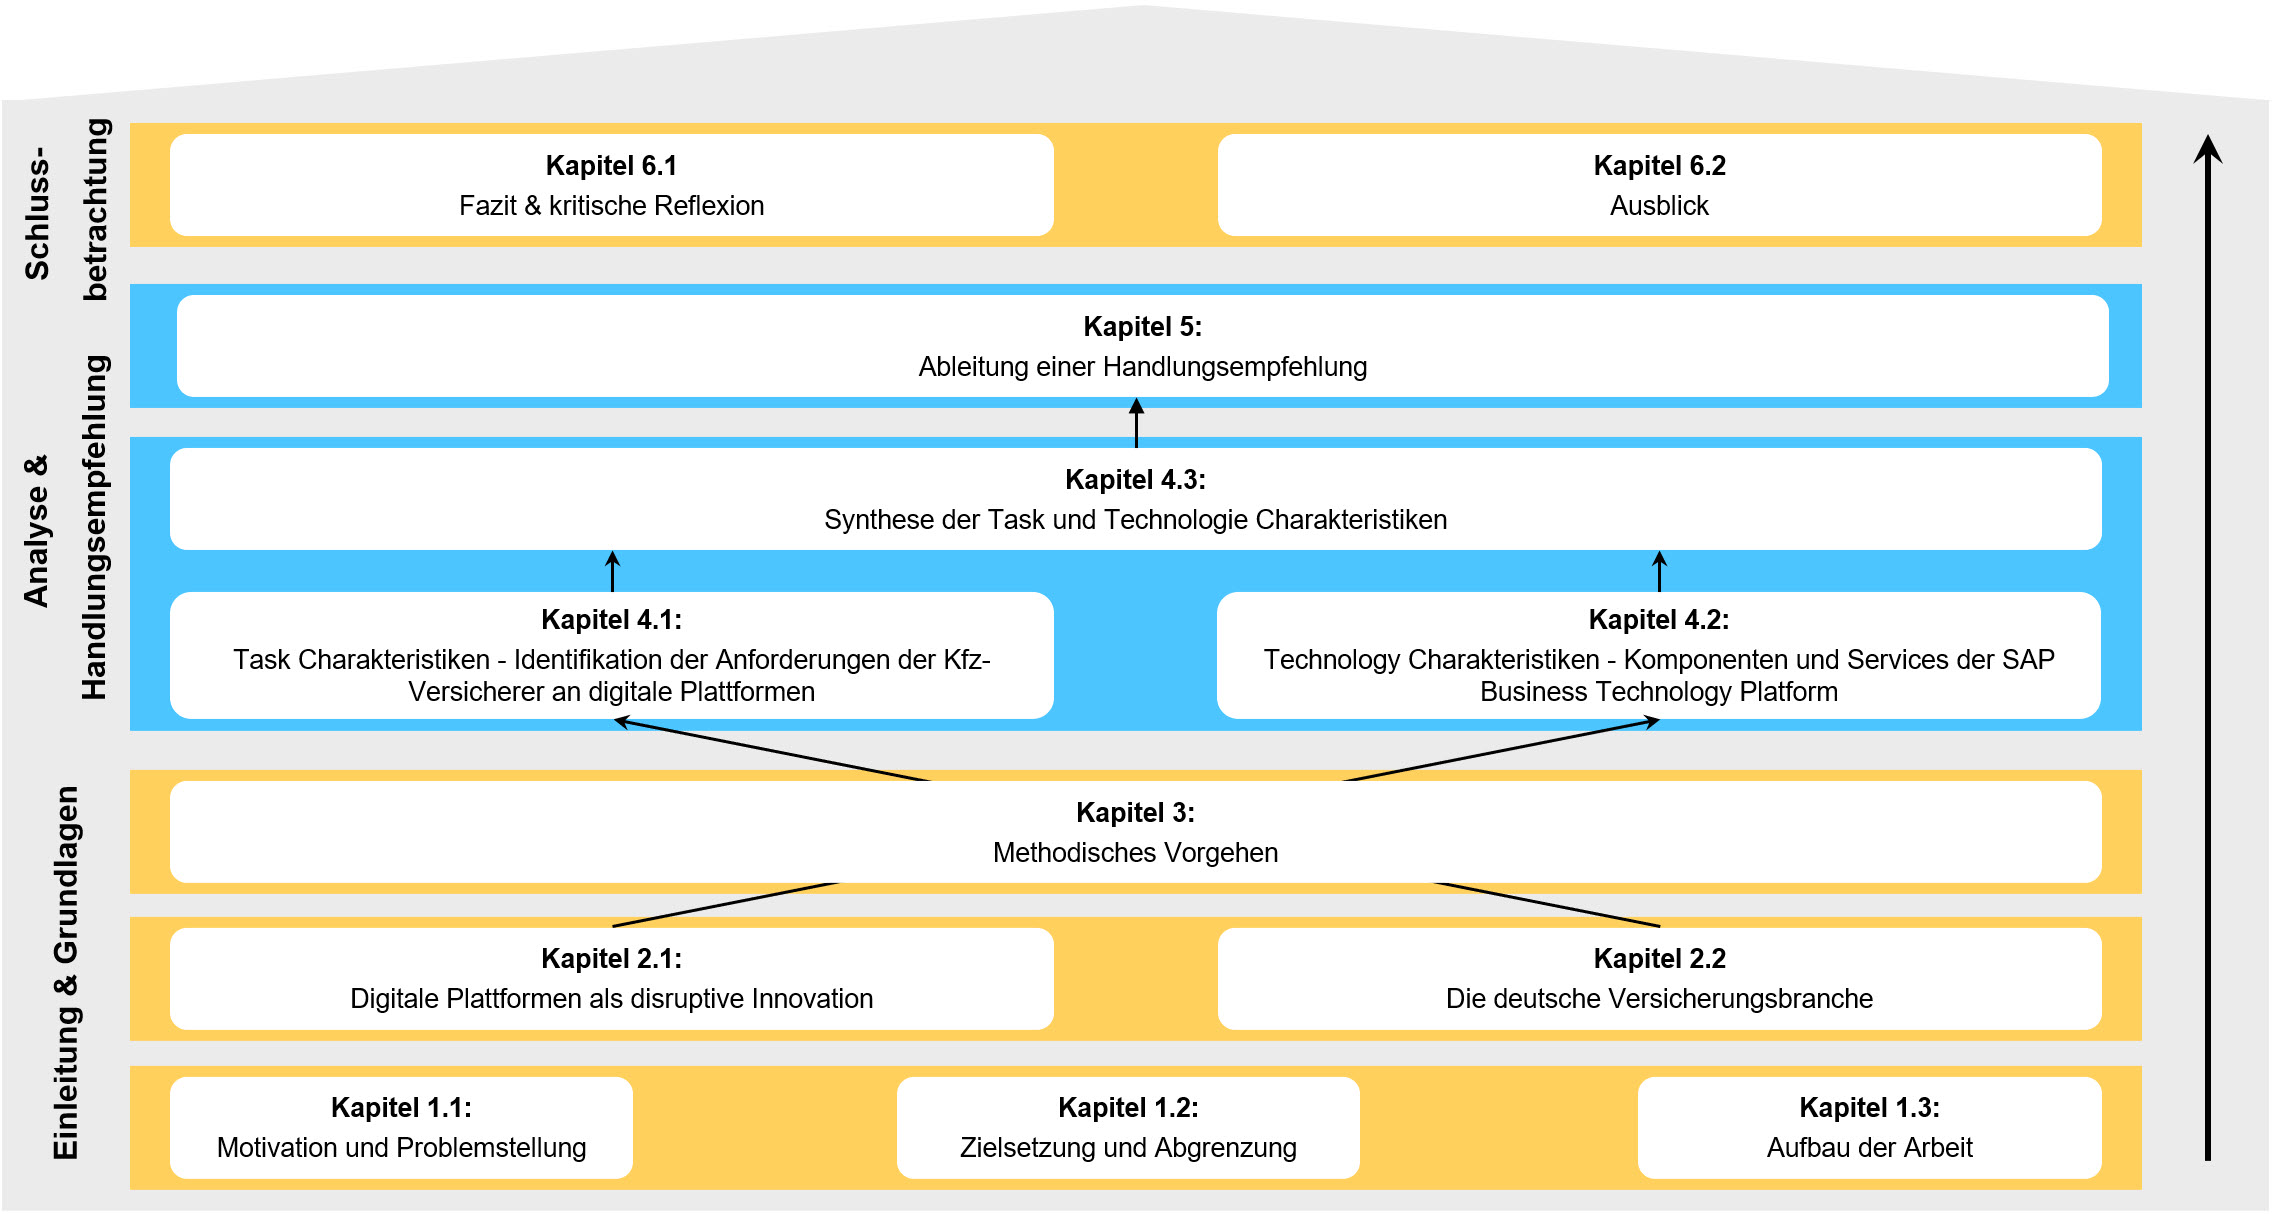
\includegraphics[width=1\textwidth]{img/Aufbau_der_Arbeit.jpg}
    \caption[Aufbau der Arbeit]{Aufbau der Arbeit\autocite{Aufbau}}
    \label{fig:Aufbau}
\end{figure}
\footnotetext{eigene Darstellung}

\improvement{Feedback Bernd: Pfeile nicht überkreuzen und Bild größer}

\newpage
%%%%%%%%%%%%%%%%%%%%%%%%%%%%%%%%%%%

%%%%%%%%%%%%%%%%%%%%%%%%%%%%%%%%%%%
% Vorgehensweise
%
% @stud: einzelne Kapitel bearbeiten und eigene Kapitel hier einfügen
%
\chapter{Grundlagen}

\section{SAP Customer Connection Programm}
%Wie unterscheide ich zwischen Ablauf und dem eigentlichen Programm

Um die Kundenzufriedenheit in Bezug zu den aktuellem \ac{plm} Applikationen zu steigern, gibt es seit Oktober 2017 das Customer Connection Programm, welches dem Kunden ermöglicht, Verbesserungsvorschläge für bestehende Softwarelösungen einzureichen und die dafür entwickelten Lösungen bereits vor offiziellem Release zu testen.\autocite[Vgl.][]{NoteCCP2021}

Das Programm richtet sich gezielt an SAP-Kunden, die bereits SAP On-Premise Lösungen benutzen, um gemeinsam mit dem Kunden neue Funktionalitäten zu erarbeiten. \autocite[Vgl.][]{CIP2021} Die Kunden können die bereits eingebrachten Vorschläge auf der Website des Customer Connection Programms einsehen und haben die Möglichkeit, für Vorschläge abzustimmen.

Sobald fünf Kunden einen Vorschlag unterstützen, wird die Umsetzungsrelevanz von einem SAP Projektteam evaluiert. Bei der Betrachtung spielen vor allem die Wichtigkeit des Vorschlags für andere Kunden, die Durchführbarkeit und die Wirtschaftlichkeit eine große Rolle. Für die Machbarkeit eines Vorschlags sind neben der Komplexität und Schwierigkeit einer Anpassung auch die verfügbaren Ressourcen von Bedeutung. Besonders gut bewertete Vorschläge werden kurzfristig, weniger interessante Kundenwünsche später realisiert oder abgelehnt. Wenn ein Kundenwunsch schon in ähnlicher Form implementiert ist, kann auch dies zur Ablehnung führen.\autocite[Vgl.][]{CCP}
\newpage
%3 Phasen mit 2 Calls in der Collect Phase
Das Programm sieht einen jährlichen Projektzyklus mit einer Gesamtlaufzeit von fünf Quartalen vor, der in verschiedene Phasen unterteilt wird.\autocite[Vgl.][]{NoteCCP2021} Zu Beginn können Kunden in der Collect Phase eigene Vorschläge einreichen und außerdem die Wünsche anderer Kunden befürworten. Je mehr Stimmen ein Vorschlag bekommt, desto wahrscheinlicher wird dessen Umsetzung. Auf die Collect Phase folgt die Selection Phase mit der Evaluierung der Kundenwünsche. Bei Fragen wird mit dem Kunden Rücksprache gehalten. Nach der erfolgreichen Umsetzung der Kundenwünsche werden während der Delivery Phase die fertigen Lösungen in Form von Hinweisen an alle relevanten SAP-Kunden ausgeliefert. Abgeschlossen wird die Delivery Phase mit der Bereitstellung eines Supportpackages, dass alle Hinweise des Projektzyklus enthält.\autocite[Vgl.][]{CCP}

%Anschließend wird in der Delivery Phase den Kunden die qualifizierten VorsIn der dritten und letzten Phase wird mit den Kick-off calls begonnen. Hier werden den Kundem die Liste der qualifizierten Vorschläge präsentiert und der Startschuss für die Umsetzung gegeben. Nach der Umsetzung des Kundenwunsches wird in Phase 4 die Lösungen an die Kunden ausgeliefert und in Delivery calls vorgestellt. In Phase 5 werden die letzten Kundenwünsche abgeschlossen und der komplette Projektzyklus wird reflektiert. Abgeschlossen wird der Projektzyklus mit dem Final call.\autocite{NoteCCP2021}\autocite{CCP}






\section{SAP PLM}


Die SAP-Applikation \acl{plm} hilft Unternehmen bei der Administration und Kontrolle des gesamten Lebenszyklus eines Produktes. Dabei werden Funktionen von der Produktentwicklung, der Herstellung über die Qualitätssicherung bis hin zu der Instandhaltung und Entsorgung abgedeckt. In der Anwendung können alle produktbezogenen Informationen verwaltet, verfolgt und überprüft werden.\autocite[Vgl.][S.232-236]{SAP01}
%sowohl im Verlauf des Produkt- und Analysezykluses als auch im Verlauf der erweiterten Logistikkette intergriert. \autocite[Vgl.][S.5]{SAPTEC}
%\autocite[Vgl.][S.232-236]{SAP01} 

Die Applikation SAP \ac{plm} kann sowohl in eine \acl{s/4hana} als auch in eine SAP-Business-Suite mit einem klassischen \ac{erp}-System integriert werden. Beide Systemlandschaften sind Geschäftsanwendungs-Paketlösungen, die eine Sammlung von betriebswirtschaftlichen Anwendungen zur Verfügung stellen. Für das Verständnis der späteren Ausführungen ist in diesem Zusammenhang vor allen Dingen bedeutsam, dass die Business-Suite \acs{s/4hana} nur mit der SAP \ac{hana} Datenbank eingesetzt werden kann und bei der Business-Suite mit klassischem \ac{erp}-System auch andere Datenbanken verwendet werden können.\autocite[Vgl.][S.4]{SAPTEC}

%Brauch man das: Durch Integration in die Business Suite können über die bestehenden Lösungsansätze in der Produktentwicklung hinaus auch Kunden und Lieferanten in erweiterte Prozessketten der Produktentwicklung miteinbezogen werden.\autocite[Vgl.][S.236]{SAP01}}

%\autocite[Vgl.][S.4]{SAPTEC}
\newpage
SAP \ac{plm} wird über ein Web User Interface bedient, dass als \ac{plmwui} bezeichnet wird. Auf der webbasierten Benutzeroberfläche können zum Beispiel Stammdaten, die den Lebenszyklus eines Produkts betreffen, angezeigt und bearbeitet werden. Zum Durchsuchen von Datenbeständen ist die \ac{plmwui}-Suche an die Enterprise Search angebunden.









\section{Technische Grundlagen}

\subsection{Enterprise Search}

Die \acl{es} wird für die einfache Suche in Business-Anwendungen wie der \ac{plmwui}-Suche benutzt und ermöglicht einen einheitlichen und sicheren Echtzeitzugriff auf Unternehmensdaten und -informationen innerhalb und außerhalb eines Unternehmens. Von der \ac{es} können sowohl strukturierte Business-Objekte wie Materialien oder Stücklisten als auch unstrukturierte Daten wie zum Beispiel PDFs aus SAP-Systemen zurückgegeben werden.\autocite[Vgl.][]{NetWeaverES} 

In der SAP-Systemlandschaft ist die Enterprise Search an den SAP NetWeaver angebunden, der als Middleware zwischen den klassischen Business-Anwendungen wie einem \ac{erp}-System und der Datenbank liegt.\autocite[Vgl.][S.13-15]{SAPTEC} Der SAP NetWeaver ist die Plattform für SAP-Geschäftsanwendungen und ermöglicht die Entwicklung, Bereitstellung und Verwaltung von SAP und nicht SAP Anwendungen in heterogenen IT-Landschaften.\autocite[Vgl.][S.8]{SAP01}


\begin{comment}
Der SAP NetWeaver ist die Plattform für SAP Geschäftsanwendungen und ermöglicht die Entwicklung, die Bereitstellung und die Verwaltung von SAP und nicht SAP Anwendungen in  heterogenen IT-Landschaften.\autocite[Vgl.][S.8]{SAP01} Als Technologie-Basis liegt SAP NetWeaver zwischen den klassischen Business-Anwendungen wie einem \ac{erp} System und der Datenbank.\autocite[Vgl.][S.24]{SAPTEC}

Als Technologie-Basis fungiert SAP NetWeaver als Mid-Wear und stellt die Kommunikation zeischen Anwendungen und Datenbank sicher.\autocite[Vgl.][S.24]{SAPTEC}


Jede dieser Business-Anwendungen kann die \ac{es} für die einfache Suche nutzen, um einen einheitlichen und sicheren Echtzeitzugriff auf Unternehmensdaten und -informationen innerhalb und außerhalb eines Unternehmens zu erlangen. Von der \ac{es} können sowohl strukturierte Business-Objekte wie Materialien oder Kundenaufträge als auch unstrukturierte Daten wie zum Beispiel PDFs aus SAP-Systemen zurückgegeben werden.\autocite[Vgl.][]{ES} 
\end{comment}



Beim Betreiben der \acl{es} wird zwischen zwei verschiedenen Suchabläufen unterschieden, die davon abhängen, ob der Kunde eine SAP \ac{hana} Datenbank oder einen anderen Suchdatenprovider nutzt. Bei den Kunden, die sich die Verbesserung gewünscht haben, kommen beide Varianten vor, weswegen nachfolgend beide Modelle vorgestellt werden.\autocite[Vgl.][]{ESV}

Der Betrieb der \acl{es} mit SAP \ac{hana} als Datenbank ermöglicht direkten Suchzugriff auf die in SAP \ac{hana} abgelegten Geschäftsdaten. Der Einsatz von weiteren Suchtechnologien ist hier nicht erforderlich.\autocite[Vgl.][]{ESV}

Beim Verwenden eines anderen, in der \ac{pam} gelisteten Suchdatenproviders ist der Anschluss der \ac{trex} erforderlich, um den fremden Suchdatenprovider im SAP System durchsuchen zu können.\autocite[Vgl.][]{ESV} 

Die Abbildung \ref{fig:ESHANA} zeigt, wie Suchanfragen bei der Anbindung von SAP \ac{hana} ausgeführt werden.


\begin{figure}[h]
    \centering
    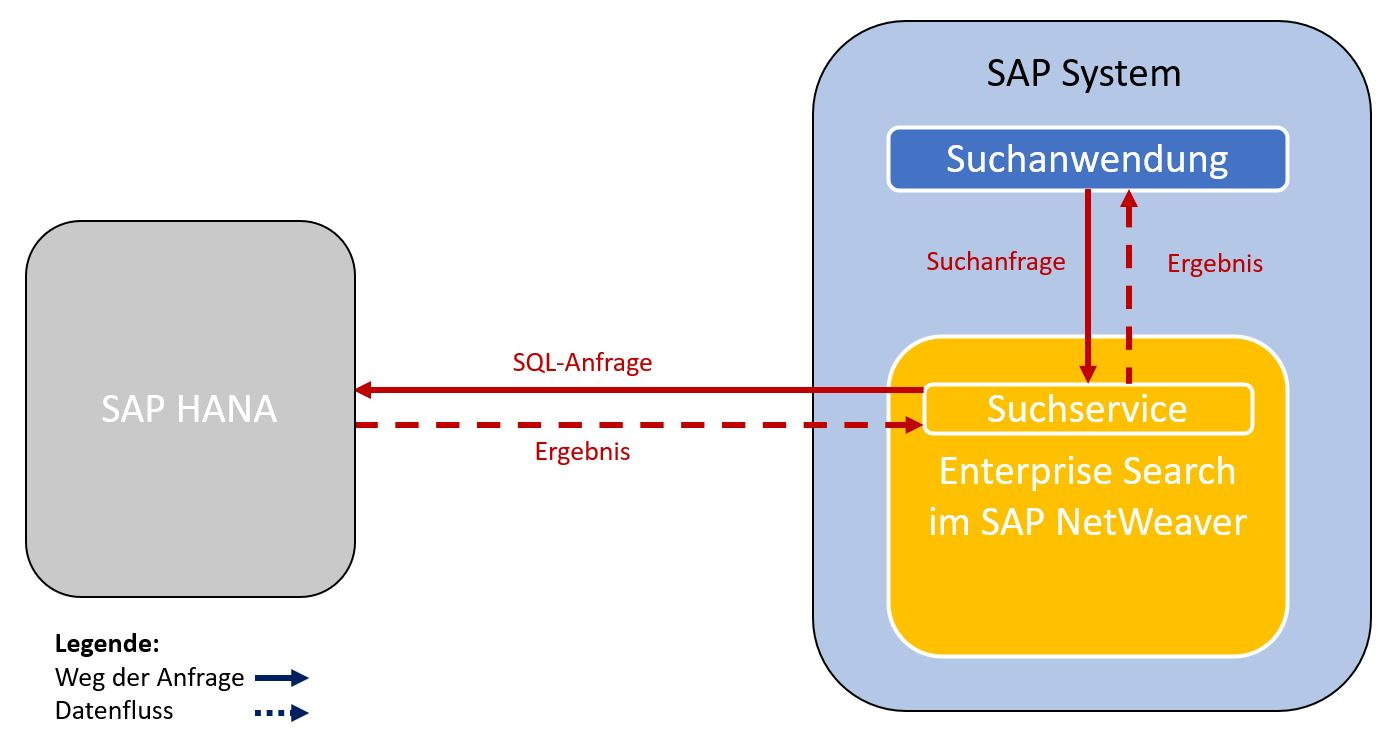
\includegraphics[width=1\textwidth]{img/ES_HANAselbst.JPG}
    \caption[ES Systemarchitektur mit SAP HANA]{ES Systemarchitektur mit SAP HANA\autocite{ESHANA}}
    \label{fig:ESHANA}
\end{figure}
\footnotetext{Vgl. eigene Darstellung angelehnt an: \textit{SAP Help Portal: ES Architektur der SAP-HANA basierten Variante 1} 2021.}

Zur Auswertung wird die Anfrage der Suchanwendung von der \ac{es} in ein \acs{sql}-Statement übersetzt.
\acs{sql} steht für Structured Query Language und wird für die Kommunikation mit Datenbanken eingesetzt. SAP HANA verarbeitet die \acs{sql}-Anfrage und gibt das Suchergebnis über die \ac{es} an die Anwendung zurück.\autocite[Vgl.][]{ESHANA}

Die Abbildung \ref{fig:ESBWA} zeigt wie Suchanfragen bei der Anbindung eines gelisteten Suchdatenproviders unter Nutzung von \ac{trex} abgewickelt werden.


Die \ac{trex} basierte Variante der Enterprise Search sucht mithilfe eines sogenannten Such-Indexes, der mögliche Suchbegriffe mit Suchergebnissen verknüpft. Zur Bildung der Indizes werden die Daten vom Suchdatenprovider mithilfe der \ac{es} extrahiert und daraufhin von \ac{trex} zu Indizes klassifiziert. Die Indizes enthalten Informationen zu dem Inhalt, dem Bearbeitungsort und der Bearbeitungsart der extrahierten Daten. Nachteil des Verfahrens ist, dass die gebildeten Such-Indizes regelmäßig aktualisiert werden müssen und das Aktualisieren sehr zeitaufwendig sein kann.\autocite[Vgl.][]{ESBWA}

\begin{figure}[h]
    \centering
    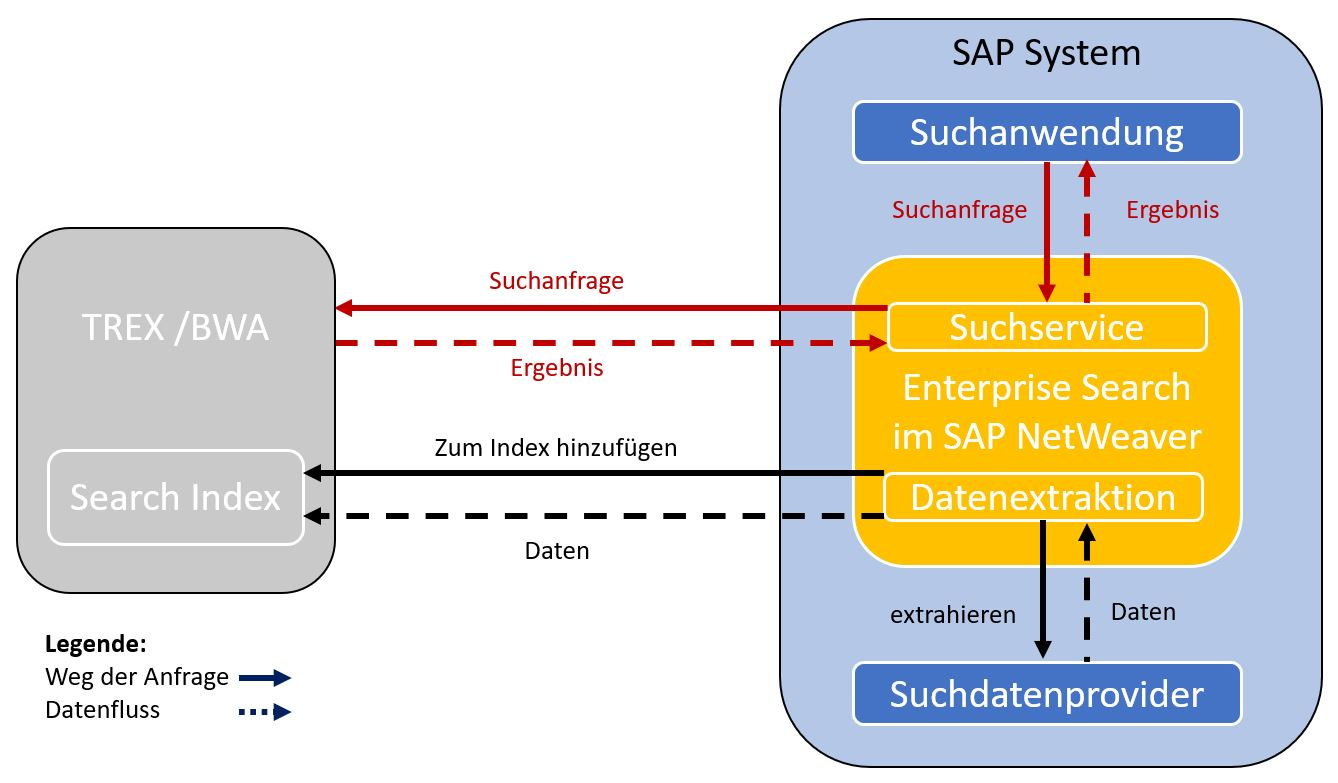
\includegraphics[width=1\textwidth]{img/ES_TREXselbstSuchdatenanbieter.JPG}
    \caption[ES Systemarchitektur mit TREX]{ES Systemarchitektur mit TREX\autocite[Vgl.]{ESBWA}}
    \label{fig:ESBWA}
\end{figure}
\footnotetext{Vgl. eigene Darstellung angelehnt an: \textit{SAP Help Portal: ES Architektur der TREX/BWA basierten Variante 1} 2021.}


\newpage
Wie in der Abbildung \ref{fig:ESBWA} zu erkennen ist, finden bei dem Verwenden eines anderen in der \ac{pam} gelisteten Suchdatenproviders zwei Abläufe statt. Bei der farblich schwarz dargestellten Extraktion und Indizierung der Daten, werden die Such-Indizes regelmäßig aktualisiert. Dazu prüft die \ac{es} die Daten zu eingeplanten Zeiten auf Änderungen. Falls sich der Datenbestand geändert haben sollte, werden die Veränderungen von \ac{trex} in die Such-Indizes aufgenommen.\autocite[Vgl.][]{ESBWA}

Die roten Pfeile zeigen den Verlauf einer Suchanfrage zur Laufzeit an. Beginnend bei der Suchanwendung wird die Anfrage von der \ac{es} an \ac{trex} weitergeleitet, um die Anfrage mit den Suchindizes abzugleichen. Die übereinstimmenden Inhalte werden anschließend als Ergebnis über die Enterprise Search an die Suchanwendung weitergegeben und dort auf der Suchoberfläche angezeigt. \autocite[Vgl.][]{ESBWA}


\begin{comment}
Zum einen das in Schwarz dargestellte extrahieren und indizierung der Daten und zum anderen der in Rot abgebildete Verlauf einer Suchanfrage zur Laufzeit. Teil der Indizierung ist das regelmäßige Aktualisieren der Such-Indizes. Dabei prüft die \ac{es} die Datenbestände zu eingeplanten Zeiten auf Änderungen und gibt diese anschließend an \ac{trex} oder \ac{bwa} weiter. Diese nehmen die Änderungen in die Such-Indizes auf.

Zur Laufzeit werden die eintreffenden Suchanfragen nicht direkt an die Datenbank weitergegeben, sondern von der \ac{es} an \ac{trex}/\ac{bwa} weitergeleitet. Daraufhin wird die Suchanfrage mit den Suchindizes abgeglichen und die übereinstimmenden Inhalte als Suchergebnis an die Enterprise Search übertragen. Letztlich wird das Ergebnis von der \ac{es} an die Suchanwendung gesendet und der Benutzer bekommt die Ergebnisse auf der Suchoberfläche angezeigt. \autocite[Vgl.][]{ESBWA}
\end{comment}
Somit ist die Enterprise Search in der Lage, Suchanfragen unabhängig von der Systemarchitektur zu verarbeiten und ein passendes Suchergebnis zurückzugeben.



\subsection{ABAP}
%alternativer Start: ABAP, was mittlerweile für Advanced Business Applikation Programming steht,ist eine von SAP entwickelte Programmiersprache zur Programmierung von kommerzielen Anwendungen im SAP Umfeld.

\acs{abap} ist die Kurzform für Advanced Business Applikation Programming und wurde zur Programmierung von kommerziellen Anwendungen im SAP-Umfeld entwickelt.
Die SAP eigene Programmiersprache gehört zu den \ac{4gl}-Sprachen und bietet dadurch viele Vorteile gegenüber elementaren Sprachen.\autocite[Vgl.][S.25]{KELLER2015}
Ein wesentlicher Unterschied von \acs{abap} zu vielen anderen Programmiersprachen ist, dass die Programme nach dem Speichern noch aktiviert werden müssen, bevor sie ausführbar sind.

\acs{abap} Programme bestehen aus einem globalen Deklarationsteil, indem die Variablen, die für das ganze Programm gültig sind, deklariert werden und einem prozeduralen Teil. Hier werden die Anweisungen, die anschließend sequenziell ausgeführt werden, implementiert.\autocite[Vgl.][S.92f]{KELLER2015} Erkennbar ist \acs{abap} insbesondere an den großgeschriebenen \acs{abap}-Schlüsselwörtern und dem Punkt am Ende jeder Befehlszeile. 

%Die Entwicklungsumgebung für ABAP Programme und alle ihre Komponenten ist die ABAP Workbench.
Eingesetzt wird \acs{abap} mithilfe der \acs{abap}-Workbench sowohl zur Entwicklung vollständig neuer Anwendungen als auch zur Erweiterung und Modifikation von SAP Standardanwendungen. Elementarer Bestandteil der \acs{abap}-Workbench, zu der eine Vielzahl von Werkzeugen zur \acs{abap}-Programmierung gehören, ist der \acs{abap}-Editor, mit welchem \acs{abap}-Programme angezeigt, geändert und ausgeführt werden können.\autocite[Vgl.][S.57,88f]{KELLER2015}

Ein wichtiges Element des \acs{abap}-Editors ist der \acs{abap}-Debugger, der die Untersuchung eines Programmcodes ermöglicht. Er eignet sich besonders gut, um die Logik des Quellcodes zu verstehen und Fehler im Programm zu finden, die die Ausführung behindern.\autocites[Vgl.][S.92-96]{S4D400}[S.87f]{GAHM2016} Beim Debuggen können zu Beispiel Rückschlüsse auf Fehler im Code durch das Anzeigen der aktuellen Werte der Variablen gezogen werden.



\subsection{Web Dynpro}
%Die WebDynpro Benutzungsoberfläche (UI) der Enterprise Search bietet einen zentralen Einstiegspunkt, um strukturierte und nicht strukturierte Daten Ihres Unternehmens aus verschiedenen Quellen mit einer einzigen Suche zu finden. \autocite{ES}
%WebDynpro steht für ... und ...
%Browser basiert , keine Installation
% (Die Anwendungen können in die Portalumgebung des SAP NetWeavers eingebunden oder von einem Browser angezeigt werden.)
%den Aufwand der Entwickler für die Erstellung leistungsfähiger Webanwendungen in einem strukturiertem Entwicklungsprozess zu minimieren. WenDynpro Anwendungen erleichtern
% Der von den Grundbausteinen generierte Quellcode wird als Web-Dynpro-Framework bezeichnet.

Die seit SAP NetWeaver 7.0 zur Verfügung stehende Web-Dynpro \acs{abap} Technologie ermöglicht die Entwicklung von \acs{abap} basierten Webanwendungen mit deklarativen Programmiertechniken. Ziel ist es, das Erstellen von \acp{ui} in der \acs{abap}-Workbench durch eine Auswahl von Grundbausteinen, die automatisch Quellcode generieren, zu erleichtern. Mit \acs{abap} Code lässt sich die zur Designzeit von Grundbausteinen aufgebaute Benutzeroberfläche für jede erforderliche Anwendungsfunktion erweiterten.\autocite[Vgl.][S.2f]{NET310}

Einer der Grundsätze der Web-Dynpro-Philosophie lautet: "Je weniger von Hand geschriebener Code, desto besser" \autocite[Vgl.][S.5]{NET310}. Das hat den großen Vorteil, dass iterative Programmieraufgaben, wie sie bei HTML und JavaScript auftreten, entfallen und folglich das Risiko auf Fehler im Programm minimiert wird.\autocite[Vgl.][S.2f]{NET310}

Web-Dynpro Anwendungen basieren auf dem Model-View-Controller Prinzip, damit die Geschäftslogik sauber von der Benutzeroberfläche getrennt werden kann. Das Prinzip teilt die zu erstellenden Programme in die Bereiche Model, View und Controller auf. \autocite[Vgl.][S.15]{NET310}

Der Model-Bereich stellt die Anwendungsdaten, auf die während der Laufzeit zugegriffen werden soll, zur Verfügung.\autocite[Vgl.][S.734]{KELLER2015}

Der View-Bereich repräsentiert den sichtbaren Teil der Anwendung und legt folglich das Design und die benötigten Web-Dynpro-Elemente fest.\autocite[Vgl.][S.15]{NET310}

Der Controller-Bereich ist für die Prozessierung der Daten zur Laufzeit verantwortlich und beinhaltet die Klassen und Methoden zur Datenverarbeitung.\autocite[Vgl.][S.734]{KELLER2015} 

\begin{figure}[h]
    \centering
    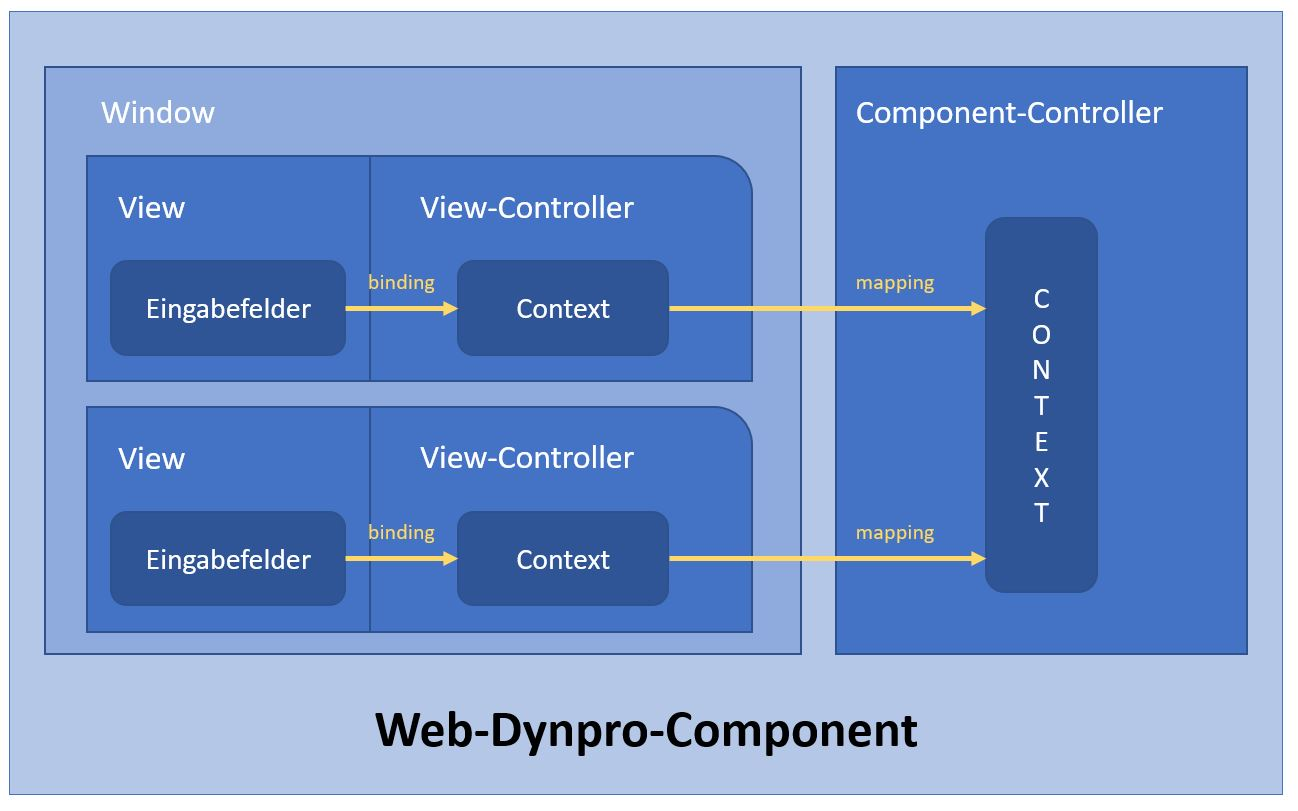
\includegraphics[width=1\textwidth]{img/WebDynpro_Componentselbst.JPG}
    \caption[Architektur eines Web-Dynpro-Components]{Architektur eines Web-Dynpro-Components\autocite[S.7]{NET310}}
    \label{fig:WebDynproComponent}
\end{figure}
\footnotetext{Vgl. eigene Darstellung angelehnt an: o.V. 2010, S.7.}


Der Rahmen einer jeden Web-Dynpro Anwendung ist der Web-Dynpro-Component. Wie in der Abbildung \ref{fig:WebDynproComponent} zu sehen, umschließt der Component als Container alle anderen Web-Dynpro-Entitäten.

%Den sichtbaren Teil einer Web-Dynpro Anwendung repräsentiert die View mit seinem Layout, dass unteranderem Eingabefelder, Labels und Drucktasten enthält, und mit dem View Designer grafisch gestaltet werden kann.

%Zu den UI bezogenen Entitäten gehören Windows und Views. Eine View ist ein Objekt ohne Schnittstelle zu "der Welt außerhalb der Component" \autocite[S.740]{KELLER2015}, weswegen es zunächst in ein Web-Dynpro-Window eingebunden werden muss. Jeder View besitzt zusätzlich zu dem Layout einen View-Controller, welcher eigene Methoden und Context-Elemente besitzt, auf welche nur der View selbst zugreifen kann. Dieser Controller steuert die View spezifische Ablauflogik, wie zum Beispiel die für die Ereignisbehandlung vorgesehenen Methoden, die nach dem Anklicken einer Schaltfläche aufgerufen werden.\autocite[Vgl.][S.738]{KELLER2015}

Der View repräsentiert dabei den sichtbaren Teil einer Web-Dynpro-Component. Das Layout des Views, das unter anderem Eingabefelder, Labels und Drucktasten enthält, kann mit dem View Designer grafisch gestaltet werden. Zusätzlich gehört zu jedem View auch ein View-Controller, auf dessen Methoden und Context-Elemente nur der View selbst zugreifen kann. Dieser Controller steuert die View spezifische Ablauflogik wie zum Beispiel die für die Ereignisbehandlung vorgesehenen Methoden, die nach dem Anklicken einer Schaltfläche aufgerufen werden.\autocite[Vgl.][S.738]{KELLER2015}

Aufgrund der Tatsache, dass der View selbst keine Schnittstelle zur "Welt außerhalb der Component hat"\autocite[S.740]{KELLER2015}, muss er zur Verwendung in ein Web-Dynpro-Window eingebunden werden. Dieses bestimmt als \ac{ui}-Container, in welcher Anordnung welche Views im Browser angezeigt werden sollen. Dabei kann ein Window eine beliebige Anzahl an Views enthalten und ein View in eine beliebige Anzahl von Windows eingebettet sein. \autocite[Vgl.][S.740]{KELLER2015}

Der in der Abbildung \ref{fig:WebDynproComponent} rechts zu sehende Component-Controller steuert die Funktionen des gesamten Components. Er ist als zentraler Controller für alle anderen Controller im Component erreichbar und enthält daher alle öffentlichen Methoden der Web-Dynpro-Component. Im Gegensatz zu den View-Controllern hat er allerdings keine visuelle Schnittstelle. \autocite[Vgl.][S.45f]{NET310}

Zu jedem Component- und View-Controller gehört jeweils ein Context, der die für die Methoden des Controllers benötigten Daten als Context-Attribute bereitstellt und unter Knoten gruppiert.\autocite[Vgl.][S.61f]{HOFFMANN2006}

%Damit die Eingaben auf der Benutzeroberfläche zu jedem Zeitpunkt mit den Context-Attributen übereinstimmen, werden die \ac{ui}-Elemente mit den Context-Attributen verknüpft. In Web-Dynpro Umfeld wird diese Verbindung als Data-Binding bezeichnet.
\newpage
Um die Eingaben auf der Benutzeroberfläche an die Methoden der Controller weitergeben zu können, müssen die entsprechenden \ac{ui}-Elemente mit den dazugehörigen Context-Attributen verknüpft sein. Diese Verbindung wird als Data-Binding bezeichnet. Zweck des Bindings ist es, den Wert des \ac{ui}-Elements zu jedem Zeitpunkt mit dem Wert des dazugehörigen Context-Attributes zu synchronisieren.\autocite[Vgl.][S.752]{KELLER2015}

Damit die View-Controller untereinander Attributwerte austauschen können, werden alle Attribute des View-Contextes auf gleichnamige Attribute im Component-Controller-Context gemappt. Ändert sich dann ein Wert eines Attributes im View-Controlller, beispielsweise durch die Eingabe eines Benutzers, werden dadurch neben den Context-Attributen des Views auch die referenzierten Attribute im Component-Controller aktualisiert.\autocite[Vgl.][S.8]{NET310}

%Jeder Web-Dynpro-Component hat außerdem als Bindeglied zwischen der Datenbank und den Controllern eine \ac{ui}-Struktur. Damit die Die \ac{ui}-Struktur legt mit vordefinierten Typen fest, wie die in der Suchoberfläche eingegebenen Daten auszusehen haben.
%Jeder Web-Dynpro-Component hat außerdem eine \ac{ui}-Struktur, die mit vordefinierten Typen festlegt, wie die in der Suchoberfläche eingegeben Daten auszusehen haben, damit die dazugehörigen Daten in der Datenbank gefunden werden können. Somit ist eine \ac{ui}-Struktur das Bindeglied zwischen Datenbanktabellen und dem Component-Controller. \change{Marco fragen}

%Durch das Data-Binding, das Context-Mapping und das Verwenden einer \ac{ui}-Struktur können die im \ac{ui} eingegebenen Daten an unterschiedliche Views, Controller und Datenbanktabellen transportiert werden. 

Das Kapseln von visuellen und programmtechnischen Web-Dynpro-Entitäten ermöglicht, dass jeder Web-Dynpro-Component in anderen Components wiederverwendet werden kann.\autocite[Vgl.][S.5]{NET310} 
%Jeder Component hat ein Interface, dass die Schnittstelle zu anderen Komponenten darstellt. Fremde Methoden und Ereignisse können im Interface-Controller bereitgestellt und mit dem visuellen Interface können auch visuelle Entitäten in die Windows anderer Components eingebunden werden.
So können in der Praxis für wiederkehrende Aufgaben wie das Anlegen eines Auftrags oder das Verwalten einer Adresse generische Components angelegt werden, die anschließend als Bausteine in andere Web-Dynpro-Anwendungen eingebettet werden. 


%%%%%%%%%%%%%%%%%%%%%%%%%%%%%%%%%%%

%%%%%%%%%%%%%%%%%%%%%%%%%%%%%%%%%%%
% Vorgehensweise
%
% @stud: einzelne Kapitel bearbeiten und eigene Kapitel hier einfügen
%
\clearpage
\chapter{Vorgehensweise}
\section{Task-Technology-Fit Theorie}

%\improvement{Einstieg Bennardo anschauen}

Das Ziel dieser Projektarbeit ist es, die Eignung der SAP BTP als digitale Plattform für Kfz-Versicherer zu untersuchen. Hierfür sollen zunächst die Anforderungen der Kfz-Versicherer an technische Plattformen identifiziert und anschließend mit den Funktionen und Services der SAP Business Technology Platform verglichen werden.

Zur Unterstützung dieser Analyse wird das Task-Technology-Fit (TTF) Modell (TTF) von Goodhue und Thompson verwendet, welches in Abblidung \ref{fig:TTF} dargestellt ist. Es vergleicht die Charakteristika einer bestimmten Aufgabe mit den Charakteristika einer bestimmten Technologie, die zur Erfüllung dieser Aufgabe verwendet werden soll. Gemäß Goodhue et. al (1995) kann eine Technologie nur dann eine positive Auswirkung auf die Leistung von Einzelpersonen oder Organisationen haben, wenn eine Übereinstimmung zwischen den Funktionalitäten der Technologie und den Anforderungen der Nutzer besteht. Die Leistungen werden umso positiver beeinflusst, je besser die Technologie mit der zu unterstützenden Aufgabe übereinstimmt.\autocite[Vgl.][S. 214-216]{GOODHUE1995}


%\autocite[Vgl.][S. 215]{GOODHUE1995}
%\autocite[Vgl.][S. 399]{SPIES2020}

\begin{figure}[h]
    \centering
    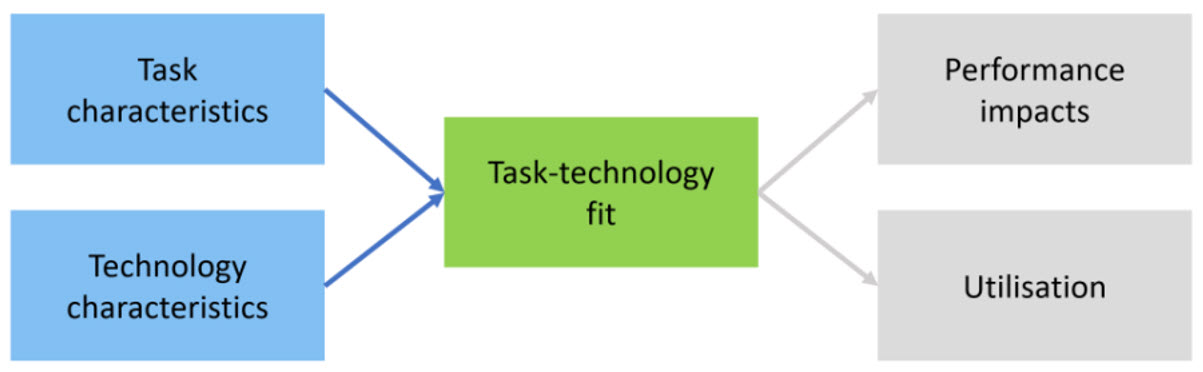
\includegraphics[width=0.9\textwidth]{img/TTF_Nadine.jpg}
    \caption[Modell der Task-Technology-Fit Theorie]{Modell der Task-Technology-Fit Theorie\autocite{TTF}}
    \label{fig:TTF}
\end{figure}
\footnotetext{Vgl. eigene Darstellung angelehnt an: Goodhue und Thompson, 1995, S. 215.}
\improvement{Frage ob man in der Grafik utilization darstellt, da es sowohl für meine Arbeit als auch für den Text nicht relevant ist}

Das TTF-Modell kann auf jeder Abstraktionsebene angewendet werden, da die aus der Anforderungsübereinstimmung resultierenden Produktivitätsverbesserungen nicht auf einzelne Personen beschränkt sind und auch für ganze Teams oder komplette Organisationen auftreten können.\autocite[Vgl.][S. 1827f]{GOODHUE1995b} 


%Hierbei kann die TTF-Analyse auf verschiedenen Abstraktionsebenen durchgeführt werden, da die Vorteile der Verbesserung der Produktivität nicht nur auf Einzelpersonen, sondern auch auf ganze Organisationen übertragen werden können.\autocite[Vgl.][S. 1827f]{GOODHUE1995b} Eine verbesserte Leistung kann gemäß TTF auf die reibungslose Ausführung der Aufgabe, die Verringerung der Kosten für die Ausführung der Aufgabe oder die Erleichterung der Aufgabe zurückzuführen. \autocite[Vgl.][S. 96]{LEE2007}

Die Task Charakteristika beziehen sich dabei auf die Gesamtheit der physischen und kognitiven Handlungen und Prozesse, welche von einer Organisation oder einer Einzelperson in einer bestimmten Umgebung ausgeführt werden. Sie werden speziell in Bezug zur Technologie, welche sie bei der Ausführung unterstützen soll, betrachtet und je nach Komplexität auf unterschiedliche Detailebenen heruntergebrochen. \autocite[Vgl.][S. 398]{SPIES2020} Nach Goodhue (1998) können die zur Evaluation der Technologie notwendigen Anforderungen mithilfe eines Task-Modells, einer Literaturrecherche oder mittels Interviews erhoben werden.\autocite[Vgl.][S. 126]{GOODHUE1998} Eine Anforderung wird in diesem Kontext definiert als eine Aussage, \enquote{die einen Bedarf und die damit verbundenen Einschränkungen und Bedingungen darstellt und erläutert}.\autocite[Vgl.][]{ISO2017}

Innerhalb des TTF-Modells beziehen sich die Technologie Charakteristika auf die Werkzeuge, welche von Einzelpersonen zur Ausführung ihrer Aufgaben verwendet werden oder diese bei der Ausführung ihrer Aufgaben unterstützen.\autocite[Vgl.][S. 399]{SPIES2020} Dabei kann sowohl der Einfluss eines einzelnen Systems, als auch die Wirkung einer Gesamtheit von bereitgestellten Systemen und Diensten betrachtet werden. \autocite[Vgl.][S. 216]{GOODHUE1995}

%Als Technologie Charakteristiken werden im Rahmen des TTF Modells die Werkzeuge bezeichnet, welche von Einzelpersonen zur Ausführung ihrer Aufgaben oder zur Unterstützung bei der Ausführung ihrer Aufgaben verwendet werden sollen.\autocite[Vgl.][S. 216]{GOODHUE1995} Dabei ist das Modell so allgemein gehalten, dass es sich entweder auf die Einfluss eines bestimmten Systems oder auf die umfassendere Wirkung der Gesamtheit der bereitgestellten Systeme, Strategien und Dienste ausgerichtet sein kann. \autocite[Vgl.][S. 399]{SPIES2020}








\newpage
\section{Systematische Literaturanalyse}


Im Rahmen des Task-Technology-Fit Models wurde eine systematische Literaturanalyse zur Identifikation der Anforderungen der Kfz-Versicherer an digitale Plattformen durchgeführt. Hierfür wurden zunächst die für die Task Charakteristika relevante Suchbegriffe auf Deutsch und Englisch festgelegt., siehe Tabelle … im Anhang. Daraufhin wurde mithilfe dieser Suchbegriffe die Datenbanken Google Scholar, EBSCO Discovery Service (aufgerufen über die Metasuche der DHBW Mannheim), JSTOR sowie WISO nach Fachliteratur, internationale und nationale Zeitschriften, Studien, Magazinen und Internetartikeln  durchsucht. Die dabei angewendeten Suchkriterien sind in Tabelle .. im Anhang aufgezeigt.  Grundlage für die Betrachtung der Recherche-Ergebnisse waren der Titel, die Kurzfassung, die Gliederung, die Einleitung sowie die Zusammenfassung der jeweiligen Quelle. Dabei wurden die ausgewählte Literatur zur Identifikation der Task Charakteristika als Ganzes oder in Ausschnitten gelesen und analysiert. (Vgl. Scrbrr)


\newpage
\section{Semistrukturiertes Leitfadeninterview und qualitative Inhaltsanalyse}

...Text kommt noch...

\newpage
%%%%%%%%%%%%%%%%%%%%%%%%%%%%%%%%%%%

%%%%%%%%%%%%%%%%%%%%%%%%%%%%%%%%%%%
% Vorgehensweise
%
% @stud: einzelne Kapitel bearbeiten und eigene Kapitel hier einfügen
%
\input{content/ist-analyse_der_suchoberfläche}
%%%%%%%%%%%%%%%%%%%%%%%%%%%%%%%%%%%

%%%%%%%%%%%%%%%%%%%%%%%%%%%%%%%%%%%
% Vorgehensweise
%
% @stud: einzelne Kapitel bearbeiten und eigene Kapitel hier einfügen
%
\chapter{Soll-Konzept und Implementierung}

\section {Analyse der bereits erweiterten Suchen}

Als Referenzmodelle für die Umsetzung des Kundenwunsches dienen die erweiterten Suchen der Rezepte, der Materialstückliste und der Dokumente, da die gewünschten Felder hier bereits implementiert wurden. Folglich können für die Anpassung der Suchoberfläche der Spezifikationen Informationen zum Vorgehen und der Umsetzung aus diesen Referenzmodellen gewonnen werden.

Zunächst wird der Aufbau des General Views untersucht, da hier viele Parallelen zu der Spezifikation erkennbar sind.
Bei der Betrachtung fällt auf, dass die Verwaltungsdaten im Layout der Referenzmodelle deckungsgleich aufgebaut sind. Alle \ac{ui}-Elemente dieses Abschnitts werden von einem Transportcontainer umfasst. Ein Transportcontainer definiert ähnlich wie ein View einen Bereich, in dem die untergeordnete Entitäten nach im Container definierten Regeln angeordnet werden.

Zu den untergeordneten Elementen gehört das Suchkriterium changed on, für das ebenfalls ein Transportcontainer angelegt wurde. In diesem Transportcontainer befinden sich zwei Eingabefelder, damit für das Änderungsdatum auch ein Zeitraum eingetragen werden kann. Vor den Eingabefeldern wurde für das Suchkriterium auch ein Label angelegt, welches die Eingabefelder im \ac{ui} beschriftet. Darauf folgen das Label und das Eingabefeld für das Suchkriterium changed by.

Den Labels wird mithilfe von \acs{otr} Texten ein Titel zugewiesen. Das Online Text Repository ist ein zentraler Ablagebereich für Texte im SAP-System. Vorteil der \acs{otr} Texte ist unter anderem, dass sich ihre Bezeichnung an die verwendete Sprache der Suchoberfläche anpasst.  

Neben den \acs{otr}-Texten ist bei der Analyse der \ac{ui}-Elementattribute aufgefallen, dass den gleichen  \ac{ui}-Bausteinen bei unterschiedlichen Referenzmodellen dieselben prozentualen Breiten und Ausrichtungen wie zum Beispiel linksbündig zugeteilt wurden. Aufgrund dieser Kongruenz empfiehlt es sich, den Aufbau und die Konfiguration der \ac{ui}-Elemente der Referenzmodelle für die Suchoberfläche der Spezifikation zu übernehmen. 

Bei der Untersuchung der Verbindungen zwischen den Web-Dynpro-Entitäten bemerkt man, dass die \ac{ui}-Strukturen der Referenzmodelle für die neuen Felder um vier weitere Komponenten erweitert wurden. Auffällig ist die Besonderheit, dass zwei der Komponenten in allen Referenzmodellen mit der Bezeichnung LOW und HIGH beginnen. Nachforschungen haben gezeigt, dass die dafür verantwortliche Methode auch bei der Spezifikation verwendet wird. Folglich sollten für die \ac{ui}-Struktur der Spezifikation zwei Komponenten mit beginnend LOW und HIGH angelegt werden, da andernfalls die Methode die Eingabefelder nicht erkennen und verarbeiten kann.

%Beim Vergleichen der Verbindungen zwischen Layout, Content und Componentcontroller, fällt auf dass die UI-Strukturen um weitere Felder, die auf der Suchoberfläche zusehen sind, erweitert wurden. Auffällig ist die Besonderheit, dass bei der normalen View für die Eingabe des Zeitraums aufgrund der zwei Inputfelder auch zwei Komponenten bei der Struktur benötigt werden, die mit LOW und HIGH beginnnen. Nachforschungen haben gezeigt, dass das an der Methode ... liegt. In der Methode, welche auch bei der Spezifikation verwendet wird, werden die zwei Datumsangaben zu einem Zeitraum verknüpft. Dafür müssen die Komponenten der UI Strukutr mit den Bezeichnungen LOW und HIGH beginnen, da andernfalls die Felder von der Methode nicht erkannt und somit auch nciht verknüpft werden können.

%Beim der Untersuchung  der \ac{ui}-Strukturen der Referenzmodelle bemerkt man, dass die \ac{ui}-Strukturen der Refenzmodelle für die neuen Felder um weitere Komponenten erweitert wurden. Die Komponenten haben zwar unterschiedliche Typen aufgrund von unterschiedlichen Datenquellen, aber immer die gleiche Beschreibung: Last Changed By und Last Changed On. Folglich müssen für die neuen Komponeten die Typen mit der gleichen Beschreibung gefunden und der \ac{ui}-Struktur der Spezifikation zugewiesen werden.\change{mit Kommentaren S. 23 abgleichen, nicht ganz rund}

Bei der Analyse des Range Views der Referenzmodelle ist die BUILD\_UP Methode aufgefallen. Diese wurde für die Einbindung der neuen Suchkriterien in die Suchoberfläche um 2 weitere Programmabschnitte erweitert. Dort werden die neuangelegten Komponenten zur Definition der Eingabedaten wiederverwendet. Für die Programmierung der erweiterten Suche der Spezifikation stellt der Code eine ausgezeichnete Vorlage dar, die es bei der Anwendung für das Objekt der Spezifikation anzupassen und zu erweitern gilt. 

Die Interfaces und Windows der Web-Dynpro-Component blieben bei den Referenzmodellen für die Funktionalität unverändert und sollten daher auch bei der Web-Dynpro-Component der Spezifikation unverändert bleiben.

%Anpassen
Bei der Untersuchung des Suchmodells der Materialstückliste in dem \ac{es}-Cockpit stellt man fest, dass die verwendeten Datenbanktabellen und Modellanfrageattribute im Vergleich zur Spezifikation andere Bezeichnungen haben, aber das Vorgehen bei der Modifikation des Suchmodells auf die Spezifikationsänderungen übertragen werden kann.

Zunächst muss für die Anbindung der Datenbanktabellen die Datenquelle in den Modellknoten festgehalten werden. Anschließend müssen die für die Suchanfrage benötigten Suchkriterien zu den Modellanfrageattributen hinzugefügt werden. Die Untersuchung der Suchmodelle für die \ac{plm}-Objekte Dokumente und Rezepte bestätigten diese Erkenntnisse.









\section{Umsetzung des Kundenwunsches}


Für die Verwirklichung des Kundenwunsches hat die Analyse der Referenzmodelle gezeigt, dass neben der Erweiterung der Suchoberfläche im Frontend auch die Modifikation der Suchmodelle im Backend notwendig ist. 
%Bei der Umsetzung wird auf die von den Referenzmodellen gewonnnenen Erkenntnisse zurückgegriffen.

%In der Dreisystemlandschaft\change{In SAPTEC als SAP-Softwarelogistik bezeichnet} bestehend aus Entwicklungs-,Qualitätssischerungs und Produktivsysteme, werden die Änderungen zunächst nur in den Entwicklungssystemen implementiert, damit der Produktivbetrieb der Systeme beim Kunden unverändert bleibt.

Zunächst werden die erforderlichen Anpassungen im Backend dargestellt. Hier wurden mit den Enterprise-Search-Tools die zur Spezifikation gehörenden Suchmodelle und Konnektoren angepasst.

Damit die Daten der neuen Suchkriterien aus der Datenbanktabelle ausgelesen werden können, wurde der Modellknoten SPEC\_KEY, um die Anfrageattribute UPDNAMS und UPDDATS erweitert. Im Modellknoten eines Suchmodells lassen sich die Spalten der Datenbanktabelle, die angebunden werden sollen, auswählen. Daraufhin wurden die zuvor genannten Attribute auch in der Modellanfrage des Suchmodells selektiert, um für die später hinzugefügten Suchfelder im \ac{plmwui} eine Suche im Index oder der Datenbank zu ermöglichen. 

Nach dem Anpassen des Suchmodells wurde über das \ac{es}-Cockpit der zum Suchmodell dazugehörige Konnektor aktualisiert. Der Konnektor stellt eine Instanz des Modells dar und verbindet den Suchdatenprovider der Applikation mit der Enterprise Search. Ohne den Konnektor ist die Suche nach Spezifikationen nicht möglich. 

%Nachdem das Backend erfolgreich geändert wurde, kann das Front-End für die Normale - und die Range View mithilfe des \ac{abap} Editors angepasst werden. Hierzu wurde zunächst die \ac{ui}-Struktur, um die Komponente UPDNAMS von Typ ESEUPDNAM und die Komponenten LOW\_UPDDATS, HIGH\_UPDDATS und UPDDATS vom Typ ESEUPDDAT erweitert. Dabei wurden die Typen der beiden neuen Komponenten der ESTRH Tabelle entnommen, die beschreibt, in welcher Form die verschiedenen Spezifikationsdaten, in der Datenbank vorliegen.

Zur Bearbeitung der Suchmasken wurde nach den Suchmodelländerungen der Web-Dynpro-Component /PLMU/WDC\_RSP\_SEA\_TAB\_ESH angepasst. Um die Struktur der Eingabedaten festlegen zu können, wurde die \ac{ui}-Struktur /PLMB/S\_RSP\_SEA\_CRIT\_BASIC\_UI, um die Komponente UPDNAMS und die Komponenten LOW\_UPDDATS, HIGH\_UPDDATS und UPDDATS erweitert. Dabei wurden die Typen der neuen Komponenten der ESTRH Tabelle entnommen, die beschreibt, in welcher Form die verschiedenen Spezifikationsdaten in den Such-Indizes oder der Datenbank vorliegen.

Anschließend wurde zur Erweiterung des Range Views der Range-View-Controller angepasst. In diesem Controller konnte mithilfe des \acs{abap}-Editors und der Vorlage aus der Referenzmodellanalyse der Quellcode der BUILD\_UP\_RSP\_RANGE Methode erweitert werden. Die Methode baut das \ac{ui} mit den Selektionsoptionen auf und definiert daher für alle Suchkriterien die dazugehörigen Elemente. Wichtig war es dabei, die genauen Bezeichnungen der \acs{otr}-Texte und Selektionshilfen zu kennen, um die richtigen Referenzen für die Suche einzutragen. 

\begin{figure}[htbp]
    \centering
    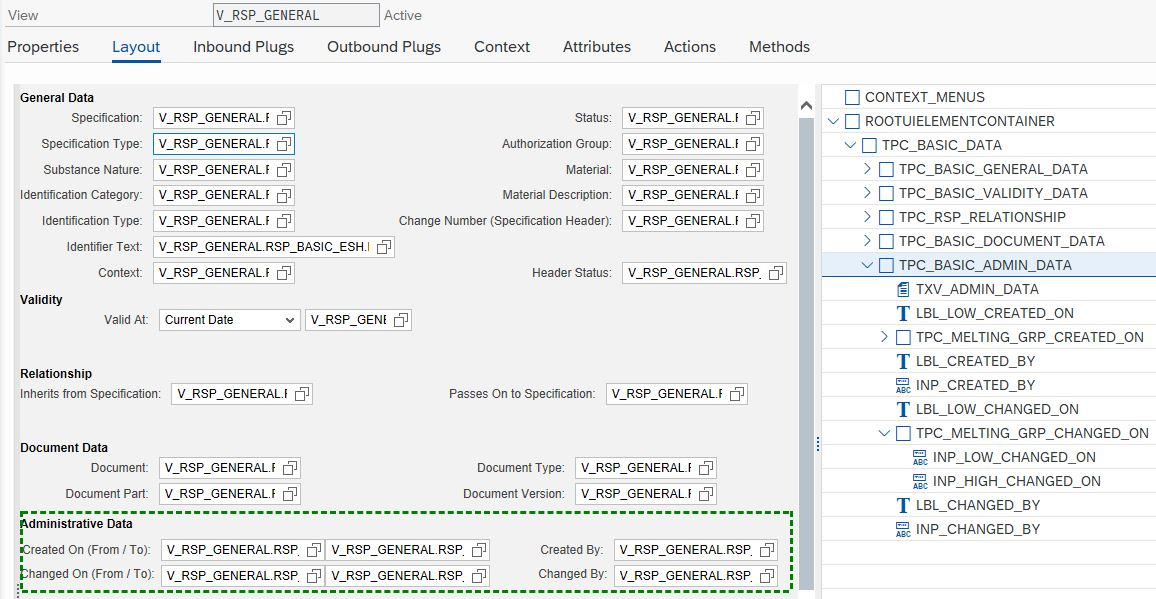
\includegraphics[width=1\textwidth]{img/NViewLayout.JPG}
    \caption[Aufbau der Suchoberfläche des General Views]{Aufbau der Suchoberfläche des General Views (Eigene Darstellung)}
    \label{fig:NViewLayout}
\end{figure}


Nach dem Erweitern des Range Views wurden die Suchkriterien changed on und changed by auch beim General View hinzugefügt. Hierzu wurde der in der Abbildung \ref{fig:NViewLayout} grün markierte Transportcontainer der Verwaltungsdaten \\TCP\_BASIC\_ADMIN\_DATA , um weitere \ac{ui}-Entitäten erweitert. Dabei war es besonders wichtig, 
die \ac{ui}-Entitäten INP\_LOW\_CHANGED\_ON und \\INP\_HIGH\_CHANGED\_ON in einem zusätzlichen Transportcontainer zu bündeln, damit die Eingabefelder wie gewünscht positioniert werden. Für den in der Abbildung \ref{fig:NViewLayout} rechts zu sehenden Aufbau des Layouts wurde auf die Erkenntnisse der Referenzmodellierung zurückgegriffen.


Um das Design der Suchoberflächen der Referenzmodelle beizubehalten, wurde insbesondere die Suchoberfläche der Materialstückliste eingehend untersucht. Hier standen vor allem die Attribute und Attributwerte der neuen Web-Dynpro-Entitäten im Vordergrund. Damit sich das \ac{ui} später dynamisch an die Größe des Screens anpassen kann und die zusammengehörenden Felder in einer Zeile dargestellt werden, wurde allen \ac{ui}-Entitäten eine prozentuale Breite zugewiesen. Darüber hinaus konnten bei der Betitelung der Labels erneut die bereits bekannten \acs{otr}-Texte wiederverwendet werden.

\begin{figure}[htbp]
    \centering
    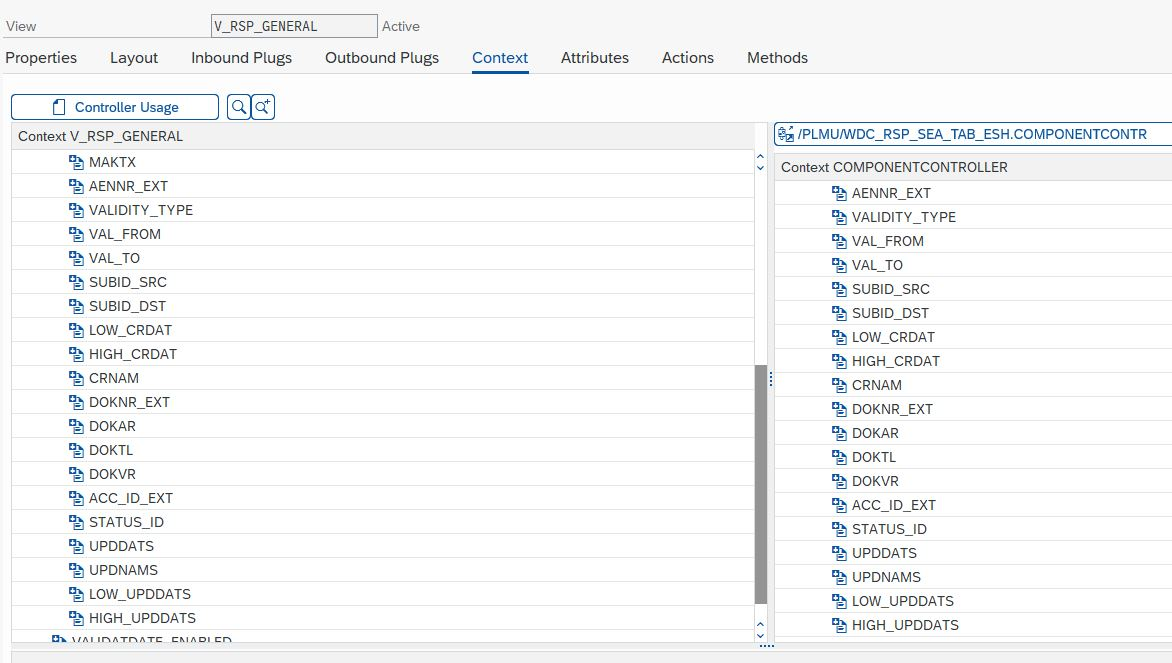
\includegraphics[width=1\textwidth]{img/ContextMapping.JPG}
    \caption[Context-Mapping zwischen dem View - und dem Component-Controller-Context]{Context-Mapping zwischen dem View - und dem Component-Controller-Context (Eigene Darstellung)}
    \label{fig:ContM}
\end{figure}

Nach der Konfiguration des Layouts war entscheidend, die Beziehungen der Web-Dynpro-Entitäten festzulegen, um das Transportieren der Eingabedaten innerhalb der Web-Dynpro-Component zu ermöglichen. Hierfür wurde zunächst das Mapping des Knotens RSP\_BASIC\_ESH im Component-Controller auf die \ac{ui}-Struktur aktualisiert, damit die neu angelegten Komponenten UPDDATS, LOW\_UPDDATS,  HIGH\_UPDDTAS und UPDNAMS für den General View zugänglich sind. Da die Context-Attribute des Component-Controllers nicht mehr mit den Context-Attributen des View-Controllers übereinstimmten, wurde das in Abbildung \ref{fig:ContM} zusehende Context-Mapping zwischen dem View-Context und dem Component-Controller-Context neu angelegt. Dadurch war es nachfolgend möglich, die Eingabefelder des Layouts mit den dazugehörigen Context-Attributen über ein Data-Binding zu verknüpfen.

Zudem waren noch analog zu den Referenzmodellen Anpassungen im Customizing für das Web \ac{ui} der Spezifikation erforderlich. Hier wurde für die Spezifikation der neue Suchbereich: RSP\_SELOPT angelegt. Für den Suchbereich wurde die Abfrageklasse /PLMI/CL\_RSP\_SEA\_CRIT\_SELOPT und \\/PLMB/CL\_SEA\_SELOPT\_CRIT\_DATA als Datenklasse mitgegeben, damit die zum Ausführen und Suchen von Daten benötigten Methoden der Suchanwendung mitgeteilt werden. Beide Klassen enthalten generische, sowie zusätzlich auf die Spezifikation zugeschnittene Methoden.

Um beide Views auf die neue Funktionalität testen zu können, wurde im Customizing über die Konfigurations-ID die zu den Views gehörenden Windows ausgewählt. Die Konfigurations-ID legt fest, welches Window beim Aufrufen der Suche im Browser angezeigt werden soll.

%Beim Testen wurden im \ac{plmwui} für die neuen Suchkriterien mehrere Werte und Wertebereiche ausgewählt und eine Suche angestoßen. Darauffolgend wurde die Liste der Ergebnisse durch Angeben zusätzlicher Sucheigenschaften weiter eingeschränkt, um das Zusammenspiel der neuen Suchkriterien mit den bereits vorhandenen überprüfen.


Zum Testen der neuen Suchfelder wurden im \ac{plmwui} zunächst einzelne Werte eingegeben und anschließend die Kriterien in Kombination mit anderen Suchkriterien getestet. Die im Webbrowser angezeigte Ergebnisliste wurde daraufhin mit den in der Datenbank vorliegenden Daten verglichen, um herauszufinden, ob die Suchanwendung vollumfänglich funktioniert.
%&Wenn die Ergebnisliste mit den Daten der Datenbank deckungsgleich ist, konnte Dadurch konnte auch bei einer Suche ohne Ergebnisse herausgefunden werden, ob für die Kombination von Suchkriterien tatsächlich kein Eintrag in der Datenbank vorliegt oder die Suchanwendung noch nicht funktioniert.

\begin{comment}
Beim Testen der Felder auf der Suchoberfläche der normalen View hat sich herausgestellt, dass für das Suchkriterium changed on keine Ergebnisse gefunden wurden, obwohl für den Zeitraum Einträge in der Datenbank vorlagen. Demzufolge wurde im \acs{abap} Editor mit dem Debuggen des Quellcodes begonnen und der erste Breakpoint in der Methode CL\_ESH\_TREX\_SEARCH gesetzt, um den Inhalt der Query zu überprüfen. (Die Query ist als Teil der ES zwischen der Suchanwendung und der Datenbank). Als Query wird die Tabelle bezeichnet, die die vom Benutzer für die Suchkriterien eingegebenen Werte, beinhaltet und das Übersetzen der Suchanfrage in ein SQL-Statement möglich macht.

Foto der Query einblenden

Nach dem eine weitere Suchanfrage gestartet wurde, konnte festgestellt werden, dass die Eingabedaten für das Feld changed on, die Query gar nicht erreichen und deshalb bei Suchanfragen nur leere Ergebnisse zurückgegeben werden. Daraufhin wurden die Methoden Schritt für Schritt durchlaufen und es hat sich herausgestellt, dass für die zwei Inputfelder des Suchkriteriums changed on zwei weitere Komponenten in der \ac{ui}-Struktur benötigt werden. Des Weiteren mussten die Komponentennamen mit LOW und HIGH beginnen, weil die Methode, die die Eingaben verarbeitet, ansonsten die beiden Datumseingaben nicht zu einem Zeitraum verknüpfen konnte.

Folglich wurde die\ac{ui}-Struktur um die Komponenten LOW\_UPDDATS und HIGH\_UPDDATS erweitert. Dabei wurde den Komponenten der Datentyp ESEUPDDAT zugewiesen, der zuvor auch für UPDDATS verwendet wurde. Anschließend mussten die Strukturänderungen durch das Aktualisieren der Mappings von Struktur zum ComponentControllerContext, von ComponentControllerContext zum ViewControllerContext und durch das Austauschen der Binding der Eingabefelder zum ViewControllerContext im WebDynpo Component verteilt werden.

% Code debuggt mit Variablen inhalten anzeigen und zusammenhänge der Methoden nach vollziehen, haben gezeigt, dass die Eingaben in der normalen View für changed on nur verarbeitet werden können wenn die vom \ac{ui} gebindetet Komponenten, die über den Componentcontroller auf die \ac{ui}-Struktur zeigen, mit LOW und HIGH beginnnen müssen. 
\end{comment}



Nachdem im Testverfahren, die Suche mit den hinzugefügten Kriterien einwandfrei funktionierte, wurden die Oberflächenanpassungen mithilfe der Transaktion SCWB in alle anderen Entwicklungssysteme der verschiedenen Releasestände transportiert. Da das Verteilen der Suchmodelländerungen nicht möglich ist, mussten in allen \ac{erp} und \acs{s/4hana} Entwicklungssystemen die Modellknoten manuell erweitert werden.


%In jedem Entwicklungssystem wird für jede Änderung am Suchmodell zur Laufzeit ein Report generiert;  Report könnte in andere Systeme transportiert werden
%Da die verschiedenen Entwicklungssysteme bei den gleichen Suchoberflächen unterschiedliche Suchkriterien haben können, lassen sich die Suchmodelländerungen nicht verteilen und mussten daher in allen \ac{erp} und \acs{s/4hana} Entwicklungsystemen manuell umgesetzt werden.


%früher hat man zu den Suchmodellen alle mglichen Felder hinzugefügt, und dann wurde darauf ein Index erzeugt
%Indixierungsprozess hat nachgeschaut, welche Felder brauchst du, sollen suchbar sein, 
%Früher müsste die Indixierungsprozess selbst geschrieben werden
% ERP Systeme: Suchmodelle von Anfang an mit vollumfänglicher Funktionalität und dafür auf maximale Effizienz im Indizierungsprozess verzichtet

%Nachdem die Übertragung der Änderungen in die verschiedenen Systeme abgeschlossen war, war es wichtig die fehlerfreie Funktionalität der neuen Felder in den Entwicklungssystemen zu kontrollieren. Die neuen Suchkriterien wurden mit mehreren Werten und Wertebereichen versehen und eine Suche angestoßen. Ebenfalls wurde die Liste der Ergebnisse durch Angeben zusätzlicher Sucheigenschaften weiter eingeschränkt um das Zusammenspiel der neuen Suchkriterien mit den bereits vorhandenen zutesten und zu überprüfen, ob die richtigen Ergebnisse dargestellt werden. Dabei hat sich herausgestellt, dass die automatische Zuweisung der Selektionshilfe bei dem Suchkriterium Changed by in der Normalen View nicht funktioniert. Infolgedessen wurde der Komponente UPDNAMS in der \ac{ui}-Struktur die ValueHelp manuell zugewiesen. Dabei konnte der Indentifikationsname der Changed on Valuehelp der Materialstückliste wiederverwendet werden. 

\begin{figure}[htbp]
    \centering
    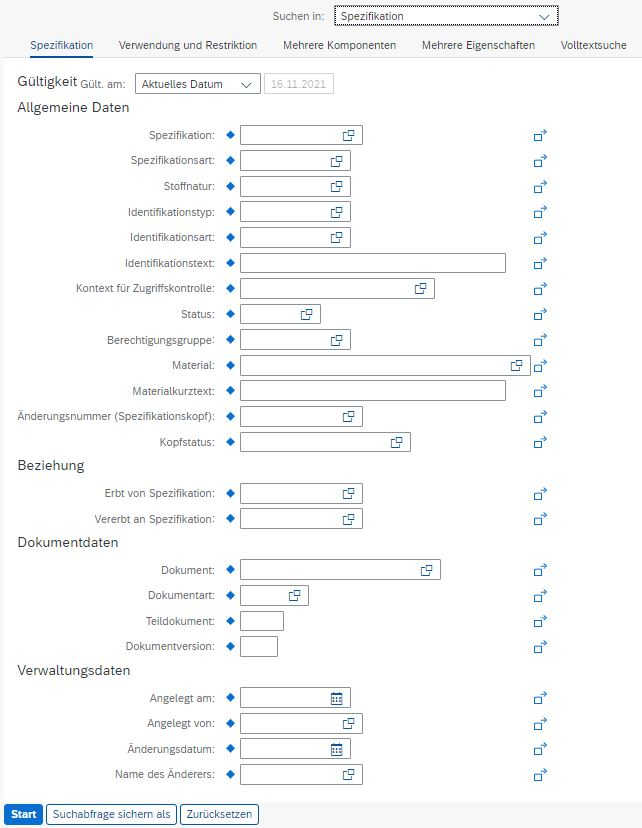
\includegraphics[width=0.9\textwidth]{img/LayoutRdanach2.jpg}
    \caption[Neue Suchoberfläche der PLM-Spezifikation im Range View]{Neue Suchoberfläche der PLM-Spezifikation im Range View (Eigene Darstellung)}
    \label{fig:Layoutfertig}
\end{figure}

Nach dem Übertragen der Anpassungen in die anderen Entwicklungssysteme war es noch einmal wichtig, das Coding und die Web-Dynpro Entitäten auch hier kurz zu überprüfen, um so die Vollständigkeit und Funktionalität der Suchoberflächen gewährleisten zu können. Anschließend war die Implementierung in den SAP-Entwicklungssystemen abgeschlossen. Das Ergebnis ist exemplarisch für den Range View in Abbildung \ref{fig:Layoutfertig} dargestellt.

Bevor die Übergabe an die Kunden erfolgen konnte, wurden die zur Auslieferung wichtigen Dokumente fertiggestellt und der Hinweis mit allen notwendigen Angaben befüllt. Dazu zählen die Information, die der Kunde zur Implementation und zum Nachvollziehen der Änderungen benötigt, sowie die Voraussetzungen, die Kundensysteme mitbringen müssen, um den Hinweis nutzen zu können.

Abschließend wurde mit dem Versenden des Hinweises und der Test Case Description die aktuell noch laufende Pilotrelease Phase angestoßen. 



%und die neue Funktionalität konnte aus den Entwicklungssystemen in die Qualitätssicherungssysteme übertragen werden.\change{auf Grafik eingehen} Dort wurden die gemachten Änderungen auf ihre Kompatiblilität mit anderen Systemen, die nicht direkt an der \ac{plmwui}-Suche beteiligt sind, überprüft, bevor die neue Funktionalität mit einem Hinweis in die Produktivsysteme der Kunden eingespielt werden konnte.

%Der Hinweis beinhaltet alle Informationen, die der Kunde benötigt, um die Änderungen bei sich erfolgreich einzuspielen. Dazu gehören Änderungen die der Kunde automatisch einspielen lassen kann, Informationen welche Hinweise der Kunde bereits benutzen muss und Anweisungen, die der Kunde nach implementieren des Hinweises noch manuell ausführen muss, um die Implementation abzuschließen. Somit hat der Kunde am Ende eine exakte Anleitung von SAP bekommen, mit der er die Lösung (zum Customer Connection Request) ohne Schwierigkeiten in seine Systeme implementieren kann.

\begin{comment}
Noch stärker differenzieren wo hat die Value Help funktioniert und wo nicht
Einleitung: Was muss umgesetzt werden 
Mögliche Themen zum ergänzen: Mandanten
Unklar wie aber Konnektoren größer aufziehen: Softwarekomponente wichtig, Status des Konnektors Möglichkeit zur Kontrolle ob dass indizieren und updaten funktioniert hat
Neben Binding Mapping erklären
Reihenfogle entscheidend
F4 Hilfe manuell hinzugefügt, da dass mit dem System nicht funktioniert hat
Testen der Funktionalität mit hilfe der ESTRH Tabelle, Datenbank im ABAPEditor anschauen:
    Hier gemachte Suchanfragen mit denen im Web \ac{ui} vergleicht und dann verglichen ob die Ergebnisse die gleichen sind, beziehungsweise ob die Spezifikationen, die mir nicht angezeigt werden, aufgrund vonmangelder Berechtigung verborgen werden oder eben die Suche noch nicht zu 100 \% funktioniert
    Welche Kombinationen ausprobiert, worauf geachtet und Sterne erklären: 
        Beachten Sie, dass sich die Suche in Dokumenten und die Suche in Textfeldern von Business-Objekten leicht unterscheiden. Textfelder werden in der Regel als Strings indiziert und Suchbegriffe müssen mit diesen Strings komplett übereinstimmen. Texte dagegen werden in einzelne Wörter aufgespalten, bevor sie indiziert werden, und selbst Wortkombinationen werden aufgespalten. Wenn Sie sicherstellen möchten, dass bei einer Suche in Business-Objekten alle Kombinationen Ihres Begriffs gefunden werden, müssen Sie ihn in Sterne setzen, z.B. *abc*. Das ist bei einer Suche in Dokumenten nicht notwendig.

Teil der Systeme als Pilotrelease an den Kunden rausgeschickt, feedback bekommen das die Note funktionier
testen imProduktivsystem

Umgehen und setzten von breakpoints

\end{comment}
%%%%%%%%%%%%%%%%%%%%%%%%%%%%%%%%%%%

%%%%%%%%%%%%%%%%%%%%%%%%%%%%%%%%%%%
% Vorgehensweise
%
% @stud: einzelne Kapitel bearbeiten und eigene Kapitel hier einfügen
%
\chapter{Fazit und Ausblick}

\section{Fazit und kritische Reflexion}

\section{Ausblick}



%%%%%%%%%%%%%%%%%%%%%%%%%%%%%%%%%%%

%\initializeAppendix %original place EditMaxD

%%%%%%%%%%%%%%%%%%%%%%%%%%%%%%%%%%%
% LITERATURVERZEICHNIS
% 
% @stud: Literaturverzeichnis in Datei bibliography.bib anpassen 
%
%\raggedright
\initializeBibliography
%%%%%%%%%%%%%%%%%%%%%%%%%%%%%%%%%%%

%%%%%%%%%%%%%%%%%%%%%%%%%%%%%%%%%%%
% ANHÄNGE
\initializeAppendix
%
% @stud: einzelne Anhänge bearbeiten und eigene Anhänge hier einfügen 
% 
\addtocontents{toc}{\protect\enlargethispage{2\normalbaselineskip}}
%% !TEX root =  master.tex
\chapter{Anhang}\label{anhang}

%\section{Konzernstruktur großer Versicherer}
%\label{sec:KonzernStrukturen}

%\begin{figure}[h]
  %\centering
  %\includegraphics[width=1\textwidth]{img/beteiligungsstruktur-axa-konzern.pdf}
  %\caption[]{AXA SE - Konzernstruktur (AXA Deutschland)}
  %\label{fig:AXAKstr}
%\end{figure}
%\newpage

\section{Suchbegriffe der Literaturanalyse}
\begin{table}[ht]
    \begin{center}
    \begin{tabular}{|p{3cm}|p{3cm}|p{3,5cm}|p{3,5cm}|}
        \hline Sprache & Suchbegriff 1 & Suchbegriff 2 & Suchbegriff 3\\[0.5ex]
        \hline Deutsch & Kfz-Versicherer, Versicherer & Anforderungen & Digitale Plattformen, technische Plattformen, PaaS, APaaS, IT-Plattformen\\
        \hline Deutsch & Kfz-Versicherer, Versicherer & Herausforderungen, Probleme & -\\
        \hline Englisch & car insurance, motor insurance, insurance & requirements & digital platforms, technological platforms, PaaS, APaaS, IT-platforms\\
        \hline Englisch & car insurance, motor insurance, insurance & challenges, problems, issues & -\\
        \hline
    \end{tabular}
    \end{center}
    \caption{Suchbegriffe der Literaturanalyse}
    \label{tab:suchbegriffe}
\end{table}  

\newpage
\section{Kriterien der Literaturanalyse}
\begin{table}[ht]
    \begin{center}
    \begin{tabular}{|p{4,33cm}|p{4,33cm}|p{4,33cm}|}
        \hline  & Einschlusskriterien & Ausschlusskriterien \\[0.5ex]
        \hline Sprache & Deutsch, Englisch & Weitere Sprachen\\
        \hline Dokumententypen & Fachliteratur, internationale und nationale wissenschaftliche Zeitschriften, Studien, Magazine, Internetartikel & Weitere Veröffentlichungen\\
        \hline Publikationszeitraum & Veröffentlichungen von 2023 - einschließlich 2013 & Veröffentlichung vor 2013\\
        \hline Verfügbarkeit & Volltext verfügbar & Volltext nicht verfügbar\\
        \hline
    \end{tabular}
    \end{center}
    \caption{Kriterien der Literaturanalyse}
    \label{tab:kriterien}
\end{table}   
\newpage

\section{Zertifizierungen der SAP BTP Services}
\label{sec:BTPZertifikate}
\begin{figure}[h]
    \centering
    \includegraphics[width=1\textwidth]{img/BTP_Zertifikate.pdf}
    %\caption[]{Zertifizierungen der SAP BTP Services (SAP SE 2023)}
    \label{fig:BTPZertifikate}
  \end{figure}
\newpage

\section{Fragenkatalog der Leitfadeninterviews}
\label{sec:Fragenkatalog}
Im laufenden Gespräch wurde die Anzahl gestellter Fragen und deren Formulierung variiert. Aufnahme und Transkription fanden über die die MS-Teams-Funktion statt.

\begin{table}[H]
\begin{tabularx}{\linewidth}{lX}
\multicolumn{2}{l}{(A) Informationsphase} \\\hline \hline 
    \    & Ich führe das Interview im Rahmen meiner Projektarbeit 2 durch, welche den Titel: \enquote{Digitale Plattformen als Wettbewerbsfaktor für den deutschen Kfz-Versicherungsmarkt am Beispiel der SAP Business Technology Platform} trägt. Das Ziel dieses Interviews ist es, Anforderungen der Kfz-Versicherer an digitale Plattformen zu identifizieren und zu priorisieren. \\\hline
    \    & Dabei sind im Rahmen meiner Arbeit mit dem Begriff digitale Plattform, technologische Plattformen gemeint, welche eine Menge von Kernprodukten, -technologien oder -services bereitstellen, auf deren Basis weitere komplementäre Produkte und Services entwickelt werden können. Somit bezeichnet der Begriff digitale Plattform im Rahmen meiner Arbeit technische Plattformen wie die SAP BTP nicht aber transaktionsorientierte Plattformen wie bspw. Uber.\\\hline
    \\     
\multicolumn{2}{l}{(B) Einstiegsphase}  \\\hline \hline
    \  1 & Welche Erfahrungen hast Du in der Versicherungsbranche? Wie sieht Dein Werdegang aus und was ist Deine aktuelle Position im Unternehmen? \\\hline     
    \\  
\multicolumn{2}{l}{(C) Hauptphase}  \\\hline \hline
    \  2 & Welche Entwicklungen waren in der Kfz-Versicherungsbranche in den letzten Jahren erkennbar und mit welchen Herausforderungen hat die Branche derzeit zu kämpfen?  \\\hline
    \  3 & Wie wirkt sich das auf die IT-Systeme in den Versicherungsunternehmen aus, bzw. welche Anforderungen lassen sich daraus an technische Plattformen ableiten? \\\hline
    \  4 & Wofür werden Deiner Einschätzung nach technologische Plattformen bei Kfz-Versicherern in den nächsten 3-5 Jahren vor allem verwendet werden? \\\hline
    \  5 & Welche Anforderungen muss eine technische Plattform für Kfz-Versicherer daher unbedingt erfüllen, bzw. welche Funktionalitäten und Services sollte eine technische Plattform aus Deiner Sicht unbedingt mitbringen, um für die Kfz-Versicherer einen Mehrwert zu schaffen?  \\\hline
    
    \end{tabularx}
    \end{table} 
    \newpage


\begin{table}[H]
\begin{tabularx}{\linewidth}{lX}
\multicolumn{2}{l}{(C) Hauptphase} \\\hline \hline
    \  6 & Eine Herausforderung der Kfz-Versicherer, von der sowohl in der Literatur als auch in der Praxis immer wieder gesprochen wird, sind die sogenannten Legacy-Systeme. Welche Anforderungen ergeben sich dadurch aus Deiner Sicht an technische Plattformen für Kfz-Versicherer? \\\hline
    \  7 & Neben den bereits genannten Punkten habe ich im Rahmen meiner Arbeit Anforderungen der Kfz-Versicherer an technische Plattformen aus der Literatur herausgearbeitet und diese zu Clustern gruppiert. Diese werde ich Dir jetzt kurz vorstellen und Dich bitten, Bezug zu den einzelnen Anforderungen zu nehmen: Kannst Du diese bestätigen und siehst Du in dem jeweiligen Cluster noch weitere Anforderungen, die für Kfz-Versicherer bei technischen Plattformen besonders wichtig sind? \\\hline       
    \  8 & Quantitativer Frageteil: Bitte priorisiere jede Anforderung auf einer Skala von 1-3 nach ihrer Wichtigkeit (1 für niedrig, 2 für mittel, 3 für hoch) für Kfz-Versicherer in den nächsten 3-5 Jahren. \\\hline
    \\
    \multicolumn{2}{l}{(D) Schlussphase}  \\\hline \hline
    \  9 & Wir sind nun am Ende des Interviews angelangt. Gibt es noch etwas, dass Du zum Thema: \enquote{Digitale Plattformen als Wettbewerbsfaktor für den deutschen Kfz-Versicherungsmarkt} hinzufügen möchtest, über das war wir noch nicht gesprochen haben? \\\hline
\end{tabularx}
    %   \captionsetup{justification=centering}
    %   \caption{Fragenkatalog -- Semistrukturiertes Experteninterview}
    %   \label{tab:fragenkatalog}
\end{table} 

\section{Auswahl der Experten}
\label{sec:Expertenwahl}
\improvement{Interview anonymisieren oder so verwerten???}
Bei der Auswahl der Experten wurde darauf geachtet, dass die Experten sowohl Erfahrung in der Kfz-Versicherungsbranche als auch über ein breites Fachwissen zu digitalen Plattformen verfügen. Alle Befragten haben bereits in Versicherungsunternehmen gearbeitet und arbeiten entweder als Berater oder IT-Architekt weiterhin mit deutschen Kfz-Versicherungsunternehmen zusammen.

Interviewpartner 1 ist Christos Lemonidis. Er kann auf mehr als 30 Jahre Erfahrung in der Versicherungsbranche zurückblicken und hat sich im Rahmen seines Studiums auf Versicherungsbetriebs- und -mathematik spezialisiert. Zudem ist er ein zertifizierter Aktuar. Vor seiner Tätigkeit bei SAP hat er in mehreren Versicherungsunternehmen gearbeitet und sich mit Themen wie Risikomanagement, IFRS, Tarifkalkulation und Rückversicherungsoptimierung, auch im Kontext von Kfz-Versicherungen, auseinandergesetzt. Seit über 16 Jahren ist er als Branchenexperte für Versicherungen bei SAP tätig und berät in dieser Funktionen Kunden zu den Kernversicherungslösungen der SAP.  

Interviewpartner 2 ist Alexander Grebert. Er ist der Global Head des Insurance Expert Teams bei SAP Fioneer, einem Joint Venture von Dediq und SAP, welches gegründet wurde, um das SAP-Portfolio für Finanzdienstleistungen gemeinsam auszubauen und in branchenspezifische Lösungen zu investieren. Vor seinem Wechsel zu SAP Fioneer hat Alexander Grebert als ehemaliger Versicherungskaufmann und Betriebswirt für Kfz-, Lebens- und Sachversicherer in Vertriebs-, Underwriting- und internen IT-Bereichen gearbeitet. Später war er als IT-Projektmanager für Erstversicherungslösungen bei der msg verantwortlich und dann in derselben Rolle für den gesamten Finanzdienstleistungssektor bei SAP. Zuletzt war er bei der SAP als \enquote{Director Insurance Architecture and Digital Transformation} tätig, bevor er im September 2021 zur SAP Fioneer wechselte.

Interviewpartner 3 ist Eduard Schmidt. Zu Beginn seiner Karriere arbeitete er in der IT-Abteilung der HDI in Hannover, wo er an der Umstellung des Bestands-, Partner- und Zahlungssystems beteiligt und für die Entwicklung von Kunden- und Vermittlerportalen verantwortlich war. Nach sechs Jahren wechselte er zur SAP und implementierte dort zunächst als Berater die Policymanagement-Lösung bei Versicherungsunternehmen, insbesondere bei Kfz-Versicherern. Heute berät er für die SAP Versicherungsunternehmen bei der Konzeptionierung und Gestaltung der Systemarchitektur.

\section{Transkription der Experteninterviews}

Von allen Teilnehmern wurde eine ausdrückliche Erlaubnis zur Transkription der Gespräche ausgestellt. Die Interviews wurden \enquote{vereinfacht} transkribiert. Das bedeutet, dass Dialekte, grammatikalische Fehler oder entbehrliche Formulierungen verbessert und Wortgenau ins Hochdeutsche übersetzt wurden.\autocite[Vgl.][S. 292]{TAUSENDPFUND2020}

\newpage
\subsection{Experteninterview 1 - Christos Lemonidis (SAP SE)}

\textit{Durchgeführt am 14.04.2023, 09:00 Uhr -- 09:39 Uhr:}


Interviewer/ Experte 1:
Teams-Programm-Test 
\#0:0:58\#

Interviewer:
Ok – dann steigen wir in das Interview ein. Zunächst vorab schon einmal vielen Dank dafür, dass du dir heute die Zeit genommen hast, mit mir das Interview zu führen. Ist es für dich in Ordnung im Rahmen meiner Projektarbeit 2 namentlich benannt zu werden oder möchtest du lieber anonym bleiben?
\#0:1:23\#

Experte 1:
Du kannst mich in deiner Projektarbeit gerne namentlich nennen.
\#0:1:29\#

Interviewer:
Alles klar, so machen wir es. Vielleicht nur so viel noch einmal zur Einleitung: Der Titel meiner Projektarbeit lautet „Digitale Plattformen als Wettbewerbsfaktor für den deutschen Kfz-Versicherungsmarkt am Beispiel der SAP Business Technology Plattform“. Das Ziel dieses Interviews ist es eben die Anforderungen der Kfz-Versicherer an digitale Plattformen zu identifizieren und danach auch zu priorisieren. Mit dem Begriff „digitale Plattformen“ sind hierbei technologische Plattformen gemeint, welche eine Menge von Kernprodukten, -technologien oder Services bereitstellen, auf deren Basis weitere Services entwickelt werden können, wie beispielsweise die SAP BTP - aber eben keine transaktionsorientierten Plattformen, wie zum Beispiel Uber. Nur so viel zur Definition, was mit dem Begriff digitale Plattform gemeint ist.
\#0:2:56\#

Experte 1:
Gut – das habe ich, soweit erst einmal verstanden.
\#0:3:01\#

Interviewer:
Ok - dann können wir also beginnen. Ich werde Dir heute im Verlauf dieses Experteninterviews 8 Fragen stellen, zu Beginn zu Deiner Person, wo Du Dich kurz vorstellen kannst, dann im Hauptteil der Fragenblock um die Anforderungen an „Digitale Plattformen“ zu identifizieren. Danach werde ich selbst einen PowerPoint-Slide auflegen mit der ich Dir die Anforderungen zeige, die ich gefunden habe. Diese dann mit Dir kurz besprechen und danach mit Dir priorisieren. Am Ende des Interviews noch eine Frage zum Ausblick. So, wenn Du keine Fragen vorab hast, würde ich jetzt mit der ersten Frage beginnen.
\#0:4:11\#

Experte 1:
Soweit keine Fragen. 
\#0:4:17\#

Interviewer:
Dann beginnen wir mit Deiner Person - welche Erfahrungen hast Du in der Versicherungsbranche und wie sieht Dein bisheriger Werdegang aus? Was ist Deine aktuelle Position im Unternehmen? Wenn Du das bitte kurz in eins bis zwei Sätzen beschreiben könntest.
\#0:4:40\#

Experte 1:
Ok - also meiner Erfahrung im Versicherungsbereich gehen tatsächlich schon knapp 30 Jahre zurück, ich hatte schon im Studium den Schwerpunkt auf Versicherungsbetriebslehre und Versicherungs¬mathematik. Ich bin seit dem Uni-Abschluss als Versicherungsmathematiker tätig und habe durch Weiterbildungen den Titel „geprüfter Aktuar der deutschen Aktuar-Vereinigung“ erlangt. Während meiner Zeit bei der Versicherung die Themen Risiko Management, IFRS, aber auch Tarifkalkulation und Rückversicherungsoptimierung gemacht. Und in diesem Rahmen habe ich mich auch mit Kfz-Tarifen auseinandergesetzt. Ja – ich bin jetzt seit 16 Jahren bei der SAP und habe auch dort den Schwerpunkt auf unseren Versicherungslösungen, insbesondere den Kern-Versicherungs¬anwendungen, wie Bestandsführungssysteme, Schadenmanagementsysteme oder Inkasso- Systemen. Genau und jetzt? Aktuell liegt mein Schwerpunkt eher Finance-and-Risk, nichtsdestotrotz sind mir natürlich die Versicherungsthemen nach wie vor gut bekannt.
\#0:5:40\#

Interviewer:
Danke - dazu kurz eine Rückfrage von mir. Du hast eben den Begriff „Aktuar-Vereinigung“ angesprochen. Was versteht man darunter, ich habe das vorher noch nicht gehört?
\#0:5:54\#

Experte 1:
Ja, genau - ein Aktuar ist der lateinische Begriff für den Versicherungsmathematiker. Er beschäftigt sich sehr sorgfältig um die Versicherungstarife und um die Versicherungsproduktion - sozusagen eben im modelltheoretischen Sinne - kümmert. Der Abschluss zum Aktuar ist eine Zusatzausbildung, die man nach dem Studium machen kann, um sich in diesem Versicherungsbereich eben noch einmal zu spezialisieren. Also so ähnlich wie bei einem Steuerberater. Diese Prüfung legt man eben bei der deutschen Aktuar Vereinigung - DAV – ab. Um den Titel dauerhaft führen zu dürfen, muss man regelmäßig Weiterbildungsveranstaltungen besuchen. Hierzu nutze ich meine jährlichen SAP-Weiterbildungsstunden, auch wenn ich aktuell im engeren Sinne als Aktuar nicht mehr tätig bin. 
\#0:6:49\#

Interviewer:
Alles klar - danke für deine Erläuterung. Jetzt können wir zu der Hauptphase des Interviews übergehen. Welche Entwicklungen waren in der Kfz-Versicherungsbranche in den letzten Jahren erkennbar und mit welchen Herausforderungen hat die Branche aktuell zu kämpfen?
\#0:7:04\#

Experte 1:
Also einerseits einmal aus der Marktsicht ist natürlich nach wie vor so, dass der Kfz-Markt hart umkämpft ist. Wir kennen wir die Werbeschlachten der einzelnen Kfz-Versicherer, die regelmäßigen Wechselspielchen am Ende jeden Jahres, die dann die „Sparfüchse“ machen. Die Kfz-Versicherung ist als Sicht der Versicherer immer noch im gewissen Sinne ein Einstiegsprodukt, um einen Versicherungskunden – im Allgemeinen -zu gewinnen. Die Kfz-Versicherung wird als „Kuppelprodukt“ angesehen. Das bedeutet, hat man ein Kfz-Versicherungsprodukt, dann kann man damit auch die anderen Versicherungsprodukte erschließen. Also ich denke, so ist die Marktsicht nach wie vor hier. Also es ist ein sehr umkämpfter Markt, wobei jetzt gerade so in den letzten 2 bis 3 Jahren hat die HUK-Coburg, die ja - so als Preisführer agiert - hier schon ihre ihrer Marktstellung ausgebaut und auch ihren Abstand auf die Allianz deutlich ausgebaut. Das kann man - meines Erachtens -schon einmal so als eine Marktbewegung einstufen. Das andere Thema sind natürlich die Telematik-Tarife und dann muss man sehen, welche in anderen Ländern deutlich mehr Fahrt aufgenommen hat, wie in Deutschland. In Deutschland sind diese Telematik-Tarife eher eine Ausnahme. Man kann sie in Deutschland eher als „Versuchsballone“ von den großen Versicherern einordnen. Bisher haben diese Telematik Tarife nicht die riesige Marktdurchdringung. Das kann man auch damit begründen, dass die Tarifwelt in Deutschland schon ziemlich ausdifferenziert ist, so dass man eine relativ große Preisspreizung zwischen risikoarmen und risikobehafteten Fahrern schon hat. Damit sind dann die Spielräume bereits relativ gering. Demzufolge ist ja auch nicht überraschend, dass Telematik Tarife – aus Versicherer-Sicht insbesondere auch für junge Fahrer attraktiv sind – ja - junge männliche Fahrer, so wie du. Die jungen männlichen Fahrer haben aus Sicht des Aktuars natürlich den höchsten Risikobedarf. Andererseits wenn diese Versichertengruppe sorgsam fahren und die das dann auch durch die Telematik-Daten nachweisen können, dass sie vorsichtige und umsichtige Fahrer sind, dann haben sie natürlich ein Hebel, auch was die Rabatte angeht. Bei den anderen Tarifen ist das so, dass da natürlich relativ wenig Spielraum in den Tarifen ist, weil das Tarifniveau in Deutschland schon relativ ausgereizt ist. Ein weiteres Thema, das für die Kfz-Versicherer dann eine Rolle spielt, dass die Autos selbst immer digitaler werden.  Der Verbrennungs¬motor, also die Leistungsklasse – wieviel kW/ PS hat das Auto, spielt ja schon immer die große Rolle, aber die Elektronikkomponenten im Auto bekommen eine immer stärkere Bedeutung, wie das früher der Fall war und das bietet natürlich dann auch Möglichkeiten im Auto - während der Fahrt - Services anzubieten und das ist natürlich auch eine Chance für Kfz-Versicherer da in das digitale Business einzusteigen. Das bedeutet, dass man sich zum Beispiel in einem Porsche elektronische Zusatz-PS dazu buchen kann, wenn man das will. So etwas könnte dann natürlich auch die Fahreigenschaften vom Auto ändern, zum Beispiel auch in Abhängigkeit des Fahrzeugstandortes, als in welchem Land wird gerade das Auto bewegt. Im internationalen Verkehr könnte man sich ja schon vorstellen, dass man dann auch entsprechenden Versicherungsschutz bietet, der sich dann der Fahrsituation oder dem Land, in dem er gerade ist, anpasst.
\#0:11:35\#

Interviewer:
Ok – das heißt zusammengefasst, dass der Markt generell sehr umkämpft in der Branche ist und Telematik-Tarife für Kfz-Versicherer ein relevantes Thema sind. Alle versuchen neue Kunden zu werben und generell wird das Auto immer vernetzter, es gibt immer mehr Daten, die man im Auto irgendwie auswerten bzw. verwenden kann. In diesem Zusammenhang die nächste Frage: Wie wirkt sich das auf die IT-Systeme in den Versicherungsunternehmen aus, bzw. welche Anforderungen lassen sich daraus denn an technische Plattformen ableiten? Sprich, was muss die Plattformen alles können und in den Bereichen unterstützen zu können.
\#0:12:08\#

Experte 1:
Also – wenn man einmal bei den Telematik-Tarifen bleibt - dann ist es so, dass da eine ganze Menge Daten verarbeitet werden müssen, also da hat man das Datentransport-Problem, aber auch das Datenverarbeitungs-Problem. Einerseits ist es natürlich so, dass Telematik-Daten sehr umfangreich sind, das ist einmal die Datenmenge und zum anderen auch das Auswertungsthema. Es nützt ja nichts, dass man die ganzen Daten nur hat, sondern man muss dann ja auch die Daten verarbeiten – also auswerten. Im Sinne von, welches sind die entscheidenden Parameter, aus denen sich dann ableiten lässt, ob ein Fahrer jetzt ein guter Fahrer oder ein risikobehafteter Fahrer ist, ob er weniger oder viel fährt etc. Also da muss man natürlich dann auch das Auswertungs-Know-how aufbauen und natürlich auch die Auswertungsmöglichkeiten dann zur Verfügung stellen. Da ist sicherlich noch einiges, was man natürlich noch nachgelagert machen kann. Aber wenn man sich vorstellt, wie dann auch ein regelmäßiger Datenfluss aus dem Auto ist und man will dann entsprechende Services mit anbieten, dann geht es ja auch darum, diese Daten in Real Time zu verarbeiten. Das heißt, dass man hier sehr zeitnah etwas dann vielleicht anbieten kann. Also ich würde ich sagen, das sind so in etwa aktuell die großen Herausforderungen aus Sicht der Kfz-Versicherer - Datenmenge. Auswertung und Echtzeitverarbeitung.
\#0:13:33\#

Interviewer:
Ok - das habe ich verstanden. Da vielleicht noch die Frage in Bezug auf die technischen Plattformen: Wofür werden, deiner Einschätzung nach, technologische Plattformen - wie die SAP BTP - bei Kfz-Versicherern in den nächsten 3-5 Jahren vor allem verwendet werden? Was erscheint denn deiner Meinung nach da am realistischsten?
\#0:14:00\#

Experte 1:
Ich glaube, dass der Bereich Telematik aus Sicht der SAP jetzt gar nicht so das Entscheidende sein wird, weil das dann schon auch so ein Spezialthema ist, in dem wir jetzt ja gar nicht so engagiert sind. Aber der ganze Themenblock „zusätzliche Services“, der spielt natürlich eine Rolle, weil man zusätzliche Services anbietet, dann muss man die ja auch abrechnen können. Und dann ist man eher in einem Customer-Experience-Umfeld oder auch einem Shop-Environment. Das ist natürlich schon etwas, was für die SAP sehr interessant sein kann. Also: Wie bringe ich die Angebote, die Services jetzt nicht aus der technischen Sicht, aber wie bekomme ich die Services auch kommerziell im Auto unter? Wie kann ich die Services über die im Auto vorhandenen Kommunikationssysteme anbieten? Und wenn die dann in Anspruch genommen wird, muss es ja auch abrechnen können. Noch einmal zu dem Beispiel „zusätzliche Porsche-PS buchen“ - “ wenn die Bereitstellung von Turbo-PS für 2 Stunden 3,70 \euro kostet, dann muss das auch irgendwo eingebucht, abgerechnet und dann auch kassiert werden. Das würde ich sagen, ist dann schon ein Geschäftsfeld für die SAP.
\#0:15:33\#

Interviewer:
Ok – du hast gerade die Punkte Funktionalität und Services angesprochen. Frage: Welche Anforderungen muss - deiner Meinung nach - eine technische Plattform für Kfz-Versicherer daher unbedingt erfüllen bzw. welche Funktionalitäten und Services sollte eine technische Plattform aus deiner Sicht unbedingt mitbringen, um für die Kfz-Versicherer einen Mehrwert zu schaffen? 
\#0:15:53\#

Experte 1:
Ja, ich glaube schon das ist das Thema Echtzeitverarbeitung - das Services-Thema muss möglichst schnell gehen und zwar in dem Moment, wo es notwendig ist. Das gleiche gilt natürlich auch für die ganzen erforderlichen betriebswirtschaftlichen Prozesse, die da dahinterstehen. Die müssen halt auch in Echtzeit dann Verfügung stehen. Also das sind jetzt keine Prozesse, wo man sich eine Batch-Verarbeitung vorstellen oder wo dann im Anschluss - irgendwie einen Tag oder Woche später - nochmal dann Papierkram erzeugt wird. Sondern das muss dann ein hochdigitaler Prozess sein, der in Echtzeit dann eben auch die Prozesse darstellt, weil das wahrscheinlich auch das ist, was dann der Konsument im Fahrzeug - in seinem „digitalen Raumschiff“ - dann auch erwartet. 
\#0:16:45\#

Interviewer:
Genau, genau - eine Herausforderung der Kfz-Versicherer, von der sowohl in der Literatur als auch in der Praxis immer wieder gesprochen wird, sind die sogenannten Legacy-Systeme. Welche Anforderungen ergeben sich dadurch aus deiner Sicht an technische Plattformen? Gibt es da Besonderheiten in Bezug auf die Alt-Systeme, die zu berücksichtigen sind ?
\#0:17:09\#

Experte 1:
Ja gut - in Bezug auf die Alt-Systeme ist doch so, dass diese oftmals so eine Echtzeitverarbeitung gar nicht darstellen können, weil die Alt-Systeme batchorientiert sind. Und dann ist natürlich die Aufgabe von einer technischen Plattform, im Gewissen Sinne auch zu entkoppeln. Ja, das sie dem Kunden gegenüber Echtzeitverarbeitung ermöglicht und aber trotzdem dann Zugriff auf die notwendigen Daten, insbesondere Stammdaten, dann auch so ein Bestandsführungssystem hat. Ja, man benötigt dann schon so eine „Entkopplungsschicht“, die natürlich dann aber auch integriert sein muss.
\#0:17:52\#

Interviewer:
Ok – nachgefragt: „Entkoppeln“ heißt in dem Punkt dann zu sagen, dass man die Alt-Systeme irgendwie versucht, zu Kapseln und dann als einen geschlossenen Baustein an die Plattform anzubinden oder wie kann ich mir die Entkopplung, die du beschrieben hast, vorstellen?
\#0:18:07\#

Experte 1:
Hm - da gehe eher einmal davon aus, dass die Alt-Systeme nur in einem beschränkten Umfang API-fähig sind. Das man sich dann Modelle überlegen muss, wie schafft man es die statischen Informationen aus dem Bestandsführungssystem einzubinden bzw. zu verwenden, auch für die Services und die Services eben dann kundenorientiert auszuprägen und auf der anderen Seite die Agilität, die man benötigt, um an der Kundenschnittstelle schnell und qualitativ hochwertige Services zur Verfügung stellen zu können.
\#0:19:02\#

Interviewer:
Du hast gerade eben schon das Schlagwort Schnittstellen angesprochen, gibt es hier typische Schnittstellen, die bei Alt-Systemen häufig vorzufinden sind. Aktuelle ist ja häufig State of the Art, die sogenannten REST-Schnittstellen. Früher war glaube ich auch viel SOAP im Einsatz. Hast du dazu Erfahrungen gesammelt?
\#0:19:22\#

Experte 1:
Ja, es ist ja schon so, dass die Versicherungen auch heutzutage da so einiges machen müssen. Aber das sind dann oft auch so Kupplungsarchitekturen, die bereits in einem Versicherungsunternehmen jetzt schon vorhanden sind, um Kundenschnittstellensysteme mit den Backend-Systemen verbinden zu können. Ob das dann direkt immer möglich ist, es wird wahrscheinlich in dem ein oder anderen Einzelfall gehen, aber in der Regel sind da schon eben genau solche Kupplungsarchitekturen not¬wendig, um Agilität auf der einen und statische Informationen auf der anderen Seite zu verknüpfen.
\#0:20:02\#

Interviewer:
Ok - dann würde ich jetzt einmal zu meiner PowerPoint kommen: Und zwar habe ich im Rahmen meiner Arbeit aus der Literatur Anforderungen der Kfz-Versicherer an technische Plattformen herausgearbeitet, von denen einige bereits genannt wurden, und diese zur besseren Strukturierung in verschiedene Cluster eingeteilt. Diese werde ich dir jetzt kurz vorstellen und dich bitten Bezug zu den einzelnen Anforderungen zu nehmen: Sprich kannst du diese bestätigen und sieht du in dem jeweiligen Cluster noch weitere Anforderungen die für Kfz-Versicherer bei technischen Plattformen besonders wichtig sind? Einen kleinen Moment - so du müsstest jetzt meinen Bildschirm sehen.
\#0:20:57\#

Experte 1:
Ja, mit der ersten Spalte Integration.
\#0:21:00\#

Interviewer:
Ganz genau - so bei den Anforderungspunkten, die ich hier im Cluster „Integration“ gefunden habe und du hattest hiervon eben schon 1 bis2 genannt gehabt, sind zu nennen „Unterstützen einer service-orientierten Architektur“, um eben auch – wie du meintest - die Alt-Systeme koppeln zu können bzw. kapseln zu können.  Um diese dann als Services für neuere Applikationen entsprechend zur Verfügung zu stellen. Die Alt-Systeme müssen eben an die neuen Plattformen angebunden werden können, das ist eine ganz wichtige Grundvoraussetzung für die Plattformen. Diese müssen mit offenen Schnittstellen-Standards letztlich kompatibel sein. Ich weiß nicht, ob dir der Begriff „digitale Ökosysteme“ etwas sagt, was ja aktuell auch so ein Trendthema in der Versicherungs¬branche ist. Da ist es ja so, dass gerade mit Kunden, Partnern oder auch Drittanbietern von Applikationen der Datenaustausch sehr wichtig ist und dazu wird eben aktuell häufig auch die REST-Schnittstelle verwendet, die man hier als State-Of-The-Art bezeichnen kann. Und eben als vierten Anforderungspunkt dieses Clusterbereichs das „API Management Tool“, sprich es gibt immer mehr Schnittstellen, die müssen eben auch kontrolliert und verwaltet werden. Sprich - wer greift auf die ganzen API überhaupt zu? Dazu an dich die Frage: Kannst du die einzelnen Anforderungen bestätigen – siehst du vielleicht im Bereich „Integration“ darüber hinaus noch weitere wichtige Punkte?
\#0:22:14\#

Experte 1:
Ja, ich kann die von dir genannten Punkte so bestätigen, ich würde aber vielleicht noch den Punkt „Kopplungsarchitektur“ noch mit aufnehmen.
\#0:22:22\#

Interviewer:
Ok – dann notiere ich mir das direkt einmal - so. Das nächste Cluster wäre dann der Bereich „Entwicklung“. Da ist es, ich glaube, zum einen ganz wichtig, dass man auf diesen technischen Plattformen eben neue Anwendungen entwickeln und auch betreiben kann. Das gilt auch für mobile Anwendungen - das ist ja auch ein Thema, das aktuell immer wichtiger wird. Im Idealfall sollten auch bestehende Anforderungen erweitert werden können, um eben die einzelnen Bedarfe der Versicherer anpassen zu können. Es sind aktuell ja – gerade auch im Versicherungsbereich – die Entwicklungsressourcen sehr knapp und wenn da die technische Plattform auch gleichzeitig Low-Code- und No-Code-Werkzeuge zur Verfügung stellen kann, dann würde das sicher auch helfen, dass vielleicht die Leute aus den Fachabteilungen auch selbst einmal mit einfachen Drag-and-Drop-Systemen Erweiterungen bauen können. Als weitere Anforderung ist - auch im Bereich der Telematik-Tarife - der Punkt „Entwicklung von IoT-Anwendungen“ zu nennen. Den hattest du ja auch schon vorhin kurz angesprochen. Da wäre auch hier die Frage an dich: Hast du zu diesen Anforderungspunkten bereits Erfahrungen gesammelt? Oder gibt es vielleicht noch weitere Punkte im Bereich der Entwicklung von Applikationen für diese technische Plattform, die ich jetzt noch nicht genannt habe?
\#0:23:38\#

Experte 1:
Nein, das passt ganz gut. Den ersten Punkt würde ich vielleicht noch einmal deutlicher herausstellen. Der ist – meines Erachtens - im Vergleich zu den nachfolgenden Punkten eine ganz wichtige Anforderung. Die anderen 3 Punkte sind - sage ich einmal so – eher nach innen gerichtet sind. Aber, dass man hier mobile Anwendungen hat, das ist ja eigentlich - gerade jetzt bezogen auf Kfz - im doppelten Sinne wichtig, auch bezüglich der Kleinteiligkeit der Anwendungen. Dann vielleicht noch ein weiterer wichtiger Aspekt, dass die technische Plattform in andere oder größere Anwendungen eingebettet ist. Es ist ja nicht so, dass die Versicherung dann das führende System ist, daher ist es wichtig bestimmte Funktionalitäten dann direkt in einem Navigationssystem oder auch in ein Fahrzeug-System anbieten zu können. Daher vielleicht noch das „Einbetten in andere Anwendungen“ als zusätzlichen Anforderungspunkt. Und bei Punkt 1 ohne die Klammer um den Begriff „mobile“, weil das - meiner Meinung nach - die Kernanforderung hier ist. 
\#0:24:47\#

Interviewer:
Frage dazu: Das heißt, du würdest dann den Punkt „mobile Anwendungen“ auch als einzelnen Punkt gezielt hervorheben? 
\#0:25:09\#

Experte 1:
Ja, das finde ich eigentlich schon wichtig und wie schon gesagt, dass diese Anwendungen eingebettet sind - in andere Systeme, weil es nicht das führende System darstellen wird.
\#0:25:24\#

Interviewer:
Ok, das habe ich verstanden. Das nächste Cluster wäre der Bereich „Datenverarbeitung“. Da glaube ich, ist der Punkt „spartenübergreifende Sicht auf Daten“ ein ganz wichtiger Punkt für die Kfz-Versicherer, um eben ein besseres Kundenverständnis zu bekommen und auch den Kunden gezielte Angebote machen zu können, wie eben im Bereich von Telematik-Tarifen. Auch das „Empfangen von Sensordaten und von physischen Objekten“ ist als Anforderungspunkt für diese technischen Plattformen- wie beispielhaft bei Autos - glaub ich auch sehr wichtig. Aufgrund der unstrukturierten Datenbasis müssen Daten mit einer Extract-Transform-Load-Lösung aufbereitet werden. Oder, was du auch schon meintest, vor allem im Bereich der vernetzten Autos eben die Analyse der großen Datenmengen. Auch für dieses Cluster wieder die Frage: Siehst du weitere Anforderungen oder passt die Aufzählung soweit?
\#0:26:05\#

Experte 1:
Das passt meiner Meinung nach so, die Anforderungen sind vollständig.
\#0:26:08\#

Interviewer:
Ok, sehr gut. Mit Blick auf Zeit – wir haben noch maximal eine Viertelstunde - würde ich jetzt direkt weiter gehen. Das vierte Cluster wäre der Bereich „Prozessautomatisierung“, hier eben zum einen durch RPA. Im Rahmen der Literaturrecherche hat sich gezeigt, dass bei Versicherungen auch viele repetitive Prozesse bestehen, die trotzdem noch manuell von Mitarbeitern ausgeführt werden und eben noch nicht automatisiert sind. Sprich – da könnte man RPA ganz gut verwenden, unter anderem auch die Automatisierung von Kundeninteraktionen, gerade bei Kundenanfragen, wie zum Beispiel Versicherungspolicen abrechnen oder Schadensmeldungen durchführen, da könnte eben der Chatbot im Vergleich zum normalen Sachbearbeiter zu jederzeit antworten - und man könnte eben auch Wartezeiten vermeiden. Da wäre wiederum die Frage: Stimmst du den Anforderungspunkten im Bereich „Prozessautomatisierung“ zu, siehst du vielleicht noch weitere, die nicht genannt wurden?
\#0:27:01\#

Experte 1:
Hm, da würde ich - auch wieder unter dem Gesichtspunkt deiner eigentlichen Fragestellung – den Anforderungspunkt 14 als deutlich relevanter ansehen, wie den Punkt 13, weil – ich sage einmal so –„Prozessautomatisierung durch RPA“ ist ja eigentlich der Blick nach hinten. Das ist ja eigentlich nur dafür da bestehende Mängel der existierenden Software zu beheben. Die spielen zwar da sicherlich eine Rolle, aber im Hinblick auf digitale Prozesse ist es ja auf jeden Fall das Ziel, dass solche Nachbearbeitungen durch Roboter überhaupt erst gar nicht anfallen, sondern dass die direkt bearbeitet werden. Also das das würde ich dann noch unterschiedlich priorisieren.
\#0:27:58\#

Interviewer:
Ok, das können wir dann gleich noch machen. In dem letzten Cluster „Weitere Anforderungen“ kommen – meiner Meinung nach – noch 2 weitere wichtige Punkte. Zum einen der Punkt „grundlegende Datensicherheit“, da können die Versicherungsunternehmen – glaube ich - schlecht die Sicherheit von Systemen komplett überprüfen. Daher greifen sie auf Zertifizierungen zurück, welche zum einen im Bereich Informationssicherheit-Management-Systeme, als auch im Bereich DSGVO benannt wurden, das sind hier die beiden ISO-Normen und eben der Punkt „Vertikale und horizontale Skalierbarkeit“ -gerade um auch mit den hohen Anfragen bei Kfz-Versicherern, beispielsweise wie sie im Herbst aufgrund der vielen Tarif-Wechsel-Kündigungen stattfinden, klar zu kommen und entsprechend weitere Ressourcen im Rahmen der Skalierbarkeit zur Verfügung  zu stellen. Stimmst du meinen Anforderungen da auch zu? 
\#0:28:44\#

Experte 1:
Ja, das passt sehr gut. Also zusammenfassend – als allgemeine Anmerkung - würde ich jetzt noch einmal versuchen die einzelnen Anforderungspunkte nicht gleichberechtigt nebeneinander zu stellen, sondern entsprechend zu priorisieren. Das heißt, noch einmal die Anforderungspunkte in Vordergrund zu stellen, die dann besonders mit digitalen Versicherungsprozessen zu tun haben. 
\#0:29:21\#

Interviewer:
Warte – den Punkt meintest du gerade, würdest du bei der „Integration“ sehen – ok. Da war noch der Punkt „Einbindung in andere Systeme“ - den hattest du dem Bereich „Entwicklung“ zugeordnet– ist das richtig so?
\#0:29:43\#

Experte 1:
Hm - ich würde den Anforderungspunkt „Einbettung in andere Systeme“ nennen.
\#0:29:51\#

Interviewer:
Genau -optional würdest du hier noch die „mobilen Anwendungen“ extra – mit hoher Priorität aufführen?
\#0:30:13\#

Experte 1:
Ja, also mir ist wichtig festzuhalten, dass die aufgeführten Anforderungspunkte in jedem Fall nicht alle gleich wichtig sind für Kfz-Versicherer. 
\#0:30:23\#

Interviewer:
So dann würde ich jetzt noch einmal zum Ende unseres Interviews kurz mit dir die Punkte priorisieren wollen. Und zwar wäre es jetzt hier die Idee, wir haben jetzt hier die einzelnen Anforderungen, die eine Plattform erfüllen sollte und dann die Bitte an dich die Wichtigkeit der einzelnen Punkte von 1 bis 3 zu priorisieren und wo die eben den Kfz-Versicherern vor allen Dingen den nächsten 3 bis 5 Jahren helfen können und vielleicht bei jedem kurz mit 1-2 Sätzen kurz beschreiben, warum du den Punkt der jeweiligen Priorität zuordnest -von hoch bis niedrig.
\#0:31:01\#

Experte 1:
Okay, also, dann fangen wir mal mit Anforderung Nr. 3 an, das würde ich alles hoch einstufen. Dann das API Management Tool als mittel einstufen, die anderen 2 Punkte als niedrig.
\#0:31:28\#

Interviewer:
Die Punkte „Legacy-Systeme“ und „Serviceorientierte Architektur“ als niedrig einzustufen, weil das in der Regel schon vorhanden schon vorhanden ist oder weil es einfach generell nicht so wichtig ist, was wäre da die Erklärung?
\#0:31:37\#

Experte 1:
Das ist – meiner Meinung nach - ja ein grundsätzliches Problem, dass die Versicherer an der Stelle haben. Das würde ich jetzt nicht unbedingt aus Sicht von KFZ an eine technische Plattform in Richtung Kundenschnittstelle als wichtigste Priorität sehen – Ok?.
\#0:31:52\#

Interviewer:
Heißt das, das sind Punkte, die deiner Auffassung nach sowieso gemacht werden müssen oder siehst du das so ein bisschen nach dem Motto. „Das wird sowieso funktionieren“ Kann ich mir das etwa so vorstellen?
\#0:32:08\#

Experte 1:
Nein – ich sage einmal, das sind grundlegende Themen, mit denen sich die Versicherer beschäftigen müssen, unabhängig davon, was sie sich im Kfz-Versicherungsbereich für zusätzliche Services vorstellen.
\#0:32:21\#

Interviewer:
Ok – das heißt, du würdest: Es ist ein allgemein wichtiger Bereich, aber in Bezug auf die Plattform-Anforderungen nicht so wichtig, weil es dabei andere gibt, die in jedem Fall wichtiger sind, wie zum Beispiel die offenen Schnittstellen.
\#0:32:33\#

Experte 1:
Ja genau – so ist es.
\#0:32:35\#

Interviewer:
Ok - dann würde ich sagen, wir machen mit dem Bereich „Entwicklung“ in der Priorisierung weiter.
\#0:32:38\#

Experte 1:
Ja, dann würde ich die „mobilen Anwendungen“ nach oben - als hohe Priorität.
\#0:32:41\#

Interviewer:
Genau und das hatten wir bereits ja auch schon kurz besprochen.
\#0:32:45\#

Experte 1:
Ebenso der Punkt „Einbettung in andere Systeme“, insbesondere die mobilen Anwendungen.
\#0:32:49\#

Interviewer:
Genau. Du würdest diesen Punkt auch ganz oben, sehen?
\#0:32:53\#

Experte 1:
Ja, genau dann das den ersten Punkt „Entwicklung und Betrieb neuer Anwendungen“ dann auch bei Mittel. Der Punkt IoT-Anwendungen und die anderen 2 wieder in die Priorität niedrig.
\#0:32:58\#

Interviewer:
OK - also würdest du die Verwendung von Low-Code-/ No-Code-Werkzeugen nicht als so wichtig ansehen, weil der Bedarf nicht da ist oder weil diese noch gar nicht so weit sind, was ist da deine Begründung?
\#0:33:18\#

Experte 1:
Wie bereits gesagt, die Bewertung sollte immer aus Sicht der grundlegenden Fragestellung erfolgen. Also, was sind so die Anforderungen. Ich möchte ja vorne an der Kundenschnittstelle etwas Neues machen und wie ich das dann letztendlich umsetze, das sehe ich eher als nachrangig an. Das Entscheidende ist es ja nicht, ob er das in einem Low-Code oder No-Code umsetzt, sondern dass die Anwendung funktioniert. Das Werkzeug ist dann an der Stelle nicht entscheidend.
\#0:34:07\#

Interviewer:
Ok - und dann noch genau der Punkt „Erweiterungen bestehender Anwendungen“, den du ganz unten einsortierst. Würdest du sagen, dass die Anwendungen, die eine technische Plattform bereitstellen soll, gar nicht groß erweitert werden möchten, da der Bedarf nicht so groß ist oder weshalb ist hier die Einordnung ganz unten?
\#0:34:21\#

Experte 1:
Also erst einmal muss ja auch irgendetwas unten stehen, wenn man priorisieren will. Ich glaube nicht, dass die funktionale Erweiterung der Back-End-Systeme hier im Vordergrund steht.
\#0:34:35\#

Interviewer:
Alles klar, okay- Das habe ich verstanden. Das sind die Punkte „IoT-Anwendungen“ und „Einbettung in andere Systeme“ wichtiger. Könntest du für mich bitte noch einmal mal - in 3 bis 4 Sätzen - den Anforderungspunkt Einbettung in andere Systeme“ kurz erläutern, also was du dir darunter vorstellst?
\#0:34:48\#

Experte 1:
Also wie gesagt, das was an der Kundenschnittstelle im Fahrzeug passieren wird, da wird ja der Versicherer das führende System hinstellen. Sondern es geht darum, also wenn man das einmal aus einer Gesamtplattform-Diskussion sieht, die hast du ja ausgegrenzt, ist es immer die Frage: Wer ist der Plattformbetreiber? Ja, und da wird die Versicherung niemals der Plattformbetreiber hinsichtlich der Kfz-Services sein, sondern es geht darum, bestimmte „Versicherungs-Schnipsel“ in einer größeren Anwendung zur Verfügung zu stellen. Man muss in der Lage sein, sich auch in andere Systeme einzubetten zu können, weil man als Versicherer selbst nie das führende System sein wird.
Ich weiß nicht, ob der Kunde dann eine Versicherungs-App in seinem Navigationssystem erwartet oder ob er einfach im Rahmen von einem Service, den er da sprichwörtlich „unter der Motorhaube“ konsumieren will, die Versicherung mit dazu bekommt. Dem entsprechend muss dann der „Software-Schnipsel“ der Versicherung darauf ausgerichtet sein muss, in einem anderen System im Hintergrund wirken zu können.
\#0:36:07\#

Interviewer:
Ok – sprich: OEM macht eine Plattform und Versicherung ist mehr Partner als eigentlicher Plattform-Betreiber. Dann würde ich sagen - mit Blick auf die Zeit - kommen wir noch zum Bereich „Datenaufbereitung“. Auch hier wieder 4 Anforderungspunkte - wie würdest du diese einsortieren? „Spartenübergreifende Sicht auf Daten“ bzw. „Empfangen von Sensordaten“ - genau?
\#0:36:29\#

Experte 1:
Hm – ich würde sagen „Analyse großen Datenmengen“ nach oben, die Sensordaten als zweit wichtig und die anderen eher nachrangig, weil es wieder allgemein ist.
\#0:36:42\#

Interviewer:
Ok – dazu noch einmal die Nachfrage im Bereich „Datenaufbereitung“ - gerade in der Analyse müssen die Daten hier auch zunächst aus der unstrukturierten Form erstmal aufbereitet werden, um sie dann Analysieren zu können. Aber für dich eben trotzdem die Priorität Datenanalyse und nicht die Datenaufbereitung da?
\#0:36:58\#

Experte 1:
Ja, das sind ja allgemeine Anforderungen. Beim nächsten Punkt – das habe ich ja vorhin schon gesagt - da wird man sagen, den Punkt „Kundeninteraktion“ würde ich hoch einstufen und den Punkt „RPA-Prozessautomatisierung“ würde ich als niedrig einstufen.
\#0:37:14\#

Interviewer:
Ok - und die letzten beiden Punkte „Datensicherheit“ und „Skalierbarkeit“ – wo sind die deiner Meinung nach einzuordnen?
\#0:37:25\#

Experte 1:
Ja, da würde ich „Datensicherheit“ von der Priorität sogar hoch einstufen, wo wir uns jetzt dann auch gegenüber anderen uns differenzieren, den Punkt „Skalierbarkeit“ als mittlere Anforderung.
\#0:37:38\#

Interviewer:
Alles klar, wunderbar - dann haben wir jetzt die Priorisierung abgeschlossen. Bitte noch einmal kurz darauf schauen – ob die Anforderungen deiner Einschätzung so richtig priorisiert sind.
\#0:37:59\#

Experte 1:
Nein - ich denke die Priorisierung, die ist ja jetzt schon ausdifferenziert – das passt.
\#0:38:07\#

Interviewer:
Wunderbar - dann sind wir jetzt am Ende des Interviews angelangt. Die abschließende Frage wäre jetzt: Gibt es noch etwas zum Thema „digitale Plattformen als Wettbewerbsfaktor für den deutschen Kfz-Versicherungsmarkt“, was du noch hinzufügen möchtest, über das wir bisher noch nicht gesprochen haben?
\#0:38:24\#

Experte 1:
Nein – es wurde alles gesagt.
\#0:38:26\#

Interviewer:
Ok -  sprich da auch da alle Punkte genannt. Vielen Dank, dass du dir die Zeit genommen hast, mit mir ein Experteninterview zu führen und meinen Fragen Rede und Antwort zu stehen. Dann würde ich jetzt hier an dieser Stelle das Recording beenden – wie gesagt noch einmal herzlichen Dank!
\#0:38:42\#


\newpage

\subsection{Experteninterview 2 - Alexander Grebert (SAP Fioneer)}

\textit{Durchgeführt am 14.04.2023, 10:30 Uhr -- 11:09 Uhr:}

Interviewer/ Experte 2:
Teams-Programm-Test 
\#0:0:03\#

Interviewer:
Vielen Dank, dass du dir die Zeit nimmst mit mir dieses Experteninterview im Rahmen meiner Projektarbeit 2 durchzuführen. Ist es für dich in Ordnung hierbei namentlich benannt zu werden oder möchtest du lieber anonym bleiben?
\#0:0:10\#

Experte 2:
Nein, das ist kein Problem – die namentliche Nennung ist ok - alles im grünen Bereich.
\#0:0:12\#

Interviewer:
Ok, dann fangen wir jetzt an. Ich hatte dir ja schon einmal meinen Leitfaden für das Interview gezeigt. Vielleicht nur so viel noch einmal zur Einleitung: Der Titel meiner Projektarbeit lautet „Digitale Plattformen als Wettbewerbsfaktor für den deutschen Kfz-Versicherungsmarkt am Beispiel der SAP Business Technology Plattform“. Das Ziel dieses Interviews ist es eben die Anforderungen der Kfz-Versicherer an digitale Plattformen zu identifizieren und danach auch zu priorisieren. Mit dem Begriff „digitale Plattformen“ sind hierbei technologische Plattformen gemeint, welche eine Menge von Kernprodukten, -technologien und entsprechende Services bereitstellen, auf deren Basis weitere Services entwickelt werden können, wie beispielsweise die SAP BTP - aber eben keine transaktionsorientierten Plattformen, wie zum Beispiel Uber. Nur so viel zur Definition, was mit dem Begriff digitale Plattform gemeint ist.
\#0:0:42\#

Experte 2:
Gut, das habe ich verstanden. Okay, du wolltest wissen, was mein Versicherungsbackground ist beziehungsweise was ich bisher in der Vergangenheit angestellt habe. Ursprünglich komme ich aus der Versicherungs¬branche, ich habe zunächst Versicherungskaufmann gelernt, danach habe ich dann Versicherungs¬betriebswirtschaft und Banking studiert – mit dem Abschluss Master. Ich habe ca. 10 bis 11 Jahre bei Versicherungsunternehmen in unterschiedlichen Funktionen gearbeitet. Die Stationen waren bei Lebensversicherern, auch bei Sachversicherern - eben auch bei Kfz-Versicherern. Und war - bevor ich zur „SAP Fioneer“ gekommen bin - 16 Jahre lang bei der SAP und habe mich dann im Wesentlichen eben auch um Kernversicherungslösungen gekümmert. Einerseits in der Entwicklung, als auch eben in der Projektdurchführung, beziehungsweise im „Project delivery“. Ich habe meinen Schwerpunkt im Bereich Bestand und Vertriebssysteme. Ich war schon innenhalb der SAP der Spezialist für Versicherungen gewesen und bin es jetzt auch noch innerhalb der SAP Fioneer.
\#0:1:42\#

Interviewer:
Wunderbar – dann ist bei dir ein sehr großer Versicherungs- als auch IT-Background gegeben. Dann würde ich jetzt einmal zur Hauptphase meines Interviews übergehen. Und zwar - welche Entwicklungen waren in der Kfz-Versicherungsbranche in den letzten Jahren erkennbar und mit welchen Herausforderungen hat die Branche aktuell zu kämpfen?
\#0:1:58\#

Experte 2:
Ich geh einmal davon aus, dass sich deine Frage primär auf den deutschen Markt bezieht, weil sich der deutsche Markt im Vergleich zu den internationalen Märkten schon ein bisschen anders verhält. Ich möchte aber trotzdem kurz noch einmal auf die Internationalität an dieser Stelle eingeben. Wodurch der deutsche Markt eben geprägt ist, dass er nach wie vor eben als Eintrittskarte für eine größere Kundenbeziehung zu verstehen ist. Das heißt also, hier ist der Preiswettbewerb und der Preiskampf immer noch sehr entscheidend. Du weißt, dass es jedes Jahr dieses „Rennen“ am Ende des Jahres gibt, wo man als Kunde seine Kfz-Versicherung von A nach B übertragen kann. Jeder will irgendwie den günstigsten Preis aushandeln und das ist natürlich etwas, wodurch der Kfz-Markt in Deutschland sehr stark geprägt ist. Das heißt also auch bei vielen Versicherungsunternehmen ist das nicht notwendigerweise der Gewinnbringer, es ist oftmals die Sparte, die auch sehr defizitär ist. Ok, das ist in einem anderen Land, in dem ich jetzt beispielsweise lebe, überhaupt nicht der Fall. Ich komme aus der Schweiz - ich bin zwar Deutscher, wohne aber in der Schweiz und da gibt es diese Form von Versicherungswettbewerb nicht. Hier wollen sich die Versicherer vor allem über Dienstleistungen und komplementäre Services zu differenzieren. Da gibt es eben auch sehr viele Sachen, die kennst du so in Deutschland bei den Versicherern nicht. Also, wenn mir jetzt beispielsweise irgendwie ein Unfall passiert und ich den verschuldet habe, dann habe ich so etwas wie eine „Wildcard“ bei meiner Versicherung. Das heißt also, ich werde nicht notwendigerweise dann im Folgejahr entsprechend zurückgestuft, sondern ich habe einen Schaden frei - so ungefähr. Das ist natürlich etwas, was sich dann auch irgendwo im Preis niederschlägt. Überhaupt keine Frage, die machen das ja nicht „for free“. Du zahlst natürlich dafür, aber - wie gesagt - über solche Sachen differenzieren sich die Versicherer. Auch ist beispielsweise die Preisgestaltung in der Schweiz komplett anders. Also eine Sache, die in Deutschland aus gutem Grund undenkbar ist, dass du die Nationalität als Tarifierungs¬merkmal heranziehst. Das bedeutet, wenn jemand beispielsweise vom Balkan kommt, der typische „3er-BMW-Fahrer“, der hat in der Schweiz ein entsprechendes Manko. Das heißt, der Kunde zahlt unter Umständen eben - bei sonstigen gleichen Parametern - aufgrund seiner Herkunft, seiner Nationalität das Doppelte an Prämie. Weil statistisch halt erwiesen ist, dass diese „Kundengruppe“ eben vermehrt für bestimmte Unfallereignisse verantwortlich, also schuld ist. Wenn du den Blick dann weiter in Richtung Osten, beispielsweise in Richtung Asien wirfst, dann spielt das Thema Mobilität eine ganz andere Rolle. Dann geht es natürlich nicht ausschließlich um Kfz-Versicherungen, sondern da kommen auch ganz andere motorisierte Fahrzeuge dazu –  wie zum Beispiel die Scooters, die ganzen 2-Wheelers. Da brauchst du nur einen Blick nach Südostasien zu werfen.
\#0:5:26\#

Interviewer:
Ok - dort ist die Lage ein bisschen anders. Meine Arbeit bezieht sich ja auf den deutschen Markt. Da hast du gerade auch die Herausforderung genannt, dass das hier ein sehr umkämpfter Markt ist, wo der Preis eine sehr große Rolle spielt. Wie wirkt sich das denn auf die IT-Systeme in den Versicherungsunternehmen aus bzw. lassen sich daraus auch vielleicht Anforderungen an technischen Plattformen ableiten - also was die Plattform unbedingt können muss?.
\#0:5:43\#

Experte 2:
Also in dem Sinne, dass die technischen Plattformen - ich sag einmal - relativ einfach zu integrieren ist, sich auch in Ökosysteme eben einbringen kann. Da spielen natürlich solche Geschichten, wie Vergleichsportale oder Aggregatoren, als Vertriebskanäle eine ganz große Rolle. Also das Stichwort an der Stelle ist dann „check 24“ oder vergleichbares. Damit ergeben sich dann natürlich auch entsprechende Anforderungen an so eine Technologieplattform, was eben Laufzeitverhalten, Performance oder ähnliches angeht. Dinge, wie „Easyness“ oder „Time-to-Market“ spielen an der Stelle eine Rolle. Also ich möchte ja nicht, nur weil ich jetzt irgendeine Tarifierung anpassen oder ändern möchte, immer in ein Entwicklungsprojekt mehr oder minder abdriften und es geht auch beispielsweise darum, solche Sachen wie Realtime-Pricing zu unterstützen. Das heißt, also auf aktuelle Marktgegebenheiten eben relativ schnell zu reagieren - also eine Outside-Perspektive zu haben als Trigger. Aber auch beispielsweise Informationen, die ich in meinem eigenen Bestand habe, eben mit zu berücksichtigen, also ein adäquates Pricing aus aktueller Sicht mit Bezug auf meinem Bestand, weil ich ja nicht notwendigerweise defizitär sein möchte, aber mich natürlich auch den Wettbewerb auf der anderen Seite eben stelle. Das ist diese Outside-Perspektive, als auch die Inside-Perspektive. Ok? Das spielt natürlich eine große Rolle, wenn du das in so einem integrativen Konstrukt im Rahmen von bestehenden Ökosystemen, Vertriebskanälen, Aggregatoren, Check 24 und was man sich da immer so vorstellen kann, eben anwendest.
\#0:7:35\#

Interviewer:
OK, das habe ich verstanden - sprich Integration, offene Schnittstellen unglaublich wichtig und eben auch die Echtzeit-Datenverarbeitung, um so etwas überhaupt anbieten zu können.
\#0:7:44\#

Experte 2:
Und Performance - das ist, glaube ich, auch einer der wesentlichen Issues, einer der großen deutschen Versicherer, die die SAP bzw. die „SAP Fioneer“ als Kunde hatte, macht es jetzt, glaube ich, nicht mehr, aber die haben sehr intensiv mit Check 24 zusammengearbeitet und haben sich eben aus Performance¬gründen eine eigenständige Antragsstrecke komplett aufgebaut. Weil sie gemerkt haben, wenn sie jetzt einfach ihre bestehenden Backend-Systeme nach außen kehren würden, dass das, den Anforderungen der zusätzlichen Performance-Last, die sich daraus ergeben würde, nicht Rechnung trägt.
\#0:8:25\#

Interviewer:
Was wären denn da im Bereich Performance so klassische Anforderungen hinsichtlich Integration, Entwicklung, Datenverarbeitung, Automatisierung? Woran denkst du dabei, wenn du sagst Performance ist unglaublich wichtig?
\#0:8:42\#

Experte 2:
Also - im wesentlichen Berechnung und Tarifierung.
\#0:8:48\#

Interviewer:
OK, verstanden - sprich optimale Preis- und Risikokalkulation ist für Versicherer sehr wichtig.
\#0:9:04\#

Experte 2:
Ja, genau das generelle Laufzeitverhalten. Also wenn ich jetzt beispielsweise den Rechenkern oder ähnliches aufrufe, dass ich eben relativ schnell zum Ergebnis komme und nicht erst 30 Sekunden warten muss. Weil dann schlicht und ergreifend beispielsweise jemand abwandert. Du musst ja auch das Geschäftsmodell dir betrachten, was dann beispielsweise Check 24 oder vergleichbare Portale eben betreiben. Sie bieten dir nicht zielgerichtet nur ein Angebot, sondern unter Umständen 5 Angebote zum Vergleich an. Wenn diese 5 Angebote natürlich alle irgendwie eine „lahme Krücke“ haben, was die Tarifierung und die API-Aufrufe angeht, wirkt sich das ja auch entsprechend negativ auf Check 24 oder andere vergleichbare Portale aus.
\#0:9:42\#

Interviewer:
Ok, das habe ich verstanden - dann noch eine weitere Frage: Wofür werden - deiner Einschätzung nach - technologische Plattformen bei Kfz-Versicherern in den nächsten 3 bis 5 Jahren vor allem verwendet werden? Was könnte das sein?
\#0:9:53\#

Experte 2:
Na ja, also ich will jetzt nicht bestimmte Sachen oder Passwords überstrapazieren, aber IoT ist natürlich ein Thema - überhaupt gar keine Frage. Der Klassiker, der sich da auch mittlerweile im Markt durchgesetzt hat, ist das Thema „Pay-As-You-Drive“, also Tarife bezogen auf Kilometer oder ähnliches. Also so zu verhalten, dann auch ein adäquates Pricing anzubieten. Ich glaub das Ganze geht aber auch unter Umständen einfach noch einen Schritt weiter, als dass wir eben konsequenter die Informationen, die in einem Fahrzeug existent sind, eben dann auch für solche weitergehenden Finanzdienstleistungen-Prozesse nutzen. Also du siehst ja auch, dass beispielsweise solche Unternehmen wie Tesla, dass die den Kunden eigene Finanzdienstleistungen und Versicherungen zusammen mit ihren Fahrzeugen dann verkaufen - Ok.
\#0:10:51\#

Interviewer:
Ja – das bedeutet die Erhebung von Daten im Auto ist sehr wichtig, um die dann eben auch in den Lösungen mit verarbeiten zu können und entsprechend integrieren zu können.
\#0:11:01\#

Experte 2:
Richtig - zum Beispiel. Daraus ergeben sich auch unter Umständen ganz andere Bedürfnisse, beziehungsweise auch andere Versicherungsformen - das heißt also, brauche ich eigentlich wirklich immer den Rundumschutz am Tag, bspw. wenn das Auto davon 12 Stunden am Tag in der Garage steht.
\#0:11:21\#

Interviewer:
Ja, genau - das ist auch eine ganz entscheidende Frage. Wir hatten es gerade schon angesprochen, ganz kurz der Punkt, dass zum Beispiel auch Sensordaten verarbeitet werden müssen. Gibt es denn noch weitere Anforderungen oder Funktionalitäten und Services, die eine Plattform unbedingt mitbringen sollte, um eben bei Kfz-Versicherern in den nächsten 3 bis 5 Jahren einen Mehrwert schaffen zu können?
\#0:11:43\#

Experte 2:
Also, ich habe das ja schon einmal mit dem ersten Teil angedeutet - also für mich ist eine wichtige Anforderung, dass eben Versicherer auch in der Lage sind zu erkennen, dass sie nicht notwendiger¬weise das führende Produkt mehr anbieten, sondern dass sich das eigentlich mehr oder minder anderen Transaktionen oder anderen Gegebenheiten eben unterordnet. Ja, sprich, wenn ich Mobilität kaufe, sei es jetzt durch den Kauf eines Fahrzeuges und ich bin der Besitzer eines Fahr¬zeuges oder sei es bspw. durch die Miete eines Fahrzeuges für einen bestimmten Zeitraum, dann spielt das Thema Versicherung da natürlich auch mit rein. Das ist bis zu einem gewissen Grad natürlich auch wieder diese ganze „Pay-As-You-Go“- oder die „Pay-As-You-Drive“ Geschichte. Eigentlich läuft es darauf hinaus, dass ich Versicherungen im Prinzip konsumierbar mache und zwar dahingehend konsumierbar mache, dass ich sie eben auch mit einer Transaktion oder mit einem Gut verknüpfe. Das, glaube ich, stell eine deutlich höhere Attraktivität für den Kunden dar als das eigentliche Kernversicherungsprodukt selbst.
\#0:13:02\#

Interviewer:
Eine Herausforderung der Kfz-Versicherer, von der sowohl in der Literatur als auch in der Praxis immer wieder gesprochen wird, sind die sogenannten Legacy Systeme. Lassen sich daraus weitere Anforderungen ableiten oder Faktoren, die da für technische Plattformen besonders wichtig sind, eben in Bezug auf diese Legacy-Systeme, sprich die Alt-Systeme?
\#0:13:21\#

Experte 2:
Ja also, da war ich mir jetzt nicht ganz sicher. Ich habe ja vorhin deinen Leitfaden durchgelesen, ob wir das gleiche Verständnis haben. Also wenn es um Legacy-Systeme geht, dann bezieht sich das aus meiner Sicht im Wesentlichen eben auf die Backend-Systeme – ok. Und wenn wir jetzt über eine Technologie, wie die BTP beispielsweise, sprechen, dann ist ja die Ambition der BTP nicht notwendigerweise ein Backend-System zu ersetzen und dafür dann eine Vertragsverwaltung anzubieten. Du hast ja gesagt, du redest jetzt hier nicht von transaktionellen Systemen, sondern das ist ja eigentlich eher etwas, was komplementär zu verstehen ist – also ergänzend. So um dann beispielsweise zusätzliche Services und Integrationsmöglichkeiten eben anzubieten. Das heißt aber für mich in letzter Konsequenz, dass ich an ein Legacy-System, wenn man es denn so nach wie vor bezeichnet- ich würde es nicht Legacy System bezeichnen, sondern als existierende Systemland¬schaft oder bestehendes Backendsystem - dann ergeben sich natürlich an diese Systeme auch neue Anforderungen, die vielleicht bisher so gar nicht „auf dem Radar“ waren. Das heißt also, beispielsweise transaktionelle Funktion, eben im Sinne von Funktionsbausteinen, Services, API´s - wie auch immer - eben nach außen kehren zu können, also auch das Legacy-Systeme eben integrativer werden, in dem Sinne. Und Technologieplattformen in dem Sinne dann eben komplementär eingesetzt werden, um API-Management beispielsweise zu ermöglichen, um sich einfacher in Ökosysteme eben zu integrieren und auch besser die Time-to-Market zu unterstützen. Ein anderer Aspekt, den ich im Prinzip durch eine technische Plattform erfüllt sehe, ist, dass sie mir Zugang zu neuen Technologien bietet. Das heißt, also meine Prozesse erweitert um Bestandteile oder Inhalte, die ich so beispielsweise gar nicht notwendigerweise in meinem System abbilden kann oder will. Als Versicherer muss man ja auch „Underwriting“, also Risiko- und Antragsprüfung, betreiben – ok. Das wird auch im Kfz-Bereich bis zu einem gewissen Grad gemacht. So jetzt gibt es ja solche tollen Sachen wie AI oder künstliche Intelligenz, also irgendwelche lernenden Modelle, die mithilfe einer technischen Plattform implementiert werden und kann die als Service auch entsprechend mir zu Nutze machen. Das hilft mir dann ja auch meine vertikale Integration zu optimieren und zu verbessern. Das heißt, also auch meine Wertschöpfungskette zu optimieren. Genau und wenn ich mir jetzt das Ganze noch einmal aus dem Blickwinkel des Software-Vendors betrachte, wie beispielsweise SAP – der einen globalen Anspruch hat, da ist vielleicht noch eine andere Dimension, die du nicht notwendigerweise auf dem Radar hast. Die technische Plattform eröffnet mir natürlich auch die Möglichkeit, meinen „Core clean zu halten“, das heißt also eine Codeline mehr oder weniger für allem Kunden zur Verfügung zu stellen. Alles, was irgendwie länderspezifisches, regionsspezifisches, spartenspezifisch - was also so ein bisschen normalerweise mehr Komplexität und Variationen im Kern darstellen würde - eben auszulagern. Das ist natürlich dann auch für einen Software-Vendor sehr interessant, was das Thema Skalierbarkeit angeht, was auch die Möglichkeit angeht, eben die Lösung, beispielsweise in der Cloud konsumierbar oder ähnliches zu machen.
\#0:18:06\#

Interviewer:
Ok - mit Blick auf die Zeit möchte ich jetzt gerne die Anforderungen der Kfz-Versicherer an technische Plattformen vorstellen, die ich in der Literarturrecherche gefunden habe. Dabei habe ich diese in verschiedene Cluster eingeteilt und ich würde dich dann bitten zu den einzelnen Anforderungen kurz Bezug zu nehmen – ob du das bestätigen kannst und ob du in dem jeweiligen Cluster noch weitere Anforderungen siehst. Um danach in einem zweiten Step diese Anforderungen mit dir aus der Sicht der Kfz-Versicherer zu priorisieren. Dann teile ich jetzt einmal meinen Bildschirm – einen kleinen Moment. So - jetzt müsstest du etwas sehen können.
\#0:18:50\#

Experte 2:
Ja – das Bild ist da.
\#0:18:52\#

Interviewer:
Genau - der erste Cluster-Bereich hier ist eben der Bereich „Integration“, bei dem als Anforderungspunkte – gemäß Recherche - zu nennen sind: „Unterstützen einer serviceorientierten Architektur“, die „Anbindung von Legacy-System“ zum Unterstützen von offenen Schnittstellen¬standards – du hast auch gerade schon das Schlagwort „digitale Ökosysteme“ angesprochen, was auch so ein Trendthema ist. Es gibt es ja auch schon erste Initiativen, die - ähnlich wie im Banking mit PSD2 - versuchen, auch so Schnittstellenstandards zu schaffen für einen offenen Datenaustausch. Im Kfz-Bereich gibt es zum Beispiel die Car-Claims-API, die auch auf dem REST-Standard basiert und eben das verfügen über API-Managements-Tools um eben auch die API-Aufruf konfigurieren und verwalten zu können. Daher die Frage - würdest du bei diesen Anforderungen so mitgehen können? Kannst du die bestätigen? Siehst du vielleicht in diesem Bereich noch weitere Anforderungen, die von mir nicht genannt wurden?
\#0:20:02\#

Experte 2:
Ja würde ich so mitgehen, ich würde dir vielleicht empfehlen noch ein paar „Business-getriebene Buzzwords“ mitaufzunehmen. Ein Stichwort wäre da beispielsweise das Thema „Embedded Insurance“, weil das ist dann beispielsweise eine mögliche Repräsentanz des Themas „Integration in bestehende Ökosysteme“ - ja. Also beispielsweise ein Klassiker im Thema „Embedded Insurance“, auch wenn das relativ trivial erscheint. Aber es erzählt letztendlich die Story „Wenn du auf booking.com bis und dort eine Reise buchst, dann kannst natürlich auch noch eine entsprechende Reiseversicherung oder Ausfallversicherung oder Ähnliches mit abschließen - ok.
\#0:20:31\#

Interviewer:
Ok - das wäre dann auch so ein bisschen der Punkt „Offene Schnittstellen-Standards“ oder wo ich dann sagen würde, die Plattform muss mit anderen Partnern kompatibel sein, um eben da auch integriert werden zu können.
\#0:20:48\#

Experte 2:
Ja - also wenn du da irgendetwas schreibst, nur ein Buzzword, was dann in dem Zusammenhang auch ganz wichtig ist, ist das Embedded Insurance – ok. Das andere Thema, was du vielleicht auch in dem Zusammenhang noch einmal auf die Agenda nehmen solltest, ist das Stichwort „Open Insurance“. Die SAP, als auch die jetzt in der Folge die SAP Fioneer – wir sind in einem Verein aktiv, der nennt sich „FRIDA - das ist die „Free Insurance Data Association“.
\#0:21:12\#

Interviewer:
Ja, genau – das ist mir bekannt.
\#0:21:15\#

Experte 2:
Das steht für „Free Insurance Data Association“ und ich bin da, mehr oder minder, in dem Verein tätig, beziehungsweise bin einer der Mitgliedsvertreter aus der SAP Fioneer-Sicht heraus und das ist natürlich dann auch ein Thema, was in dem Zusammenhang sehr gut passen würde ja.
\#0:21:32\#

Interviewer:
Genau - ich habe auch bei meiner Arbeit überlegt, wie kann ich denn aus diesem Ökosystem-Gedanken gerade auch mit FRIDA eine Anforderung an eine Plattform formulieren? Und die Überlegung wäre da zu sagen: FRIDA versucht, die einzelnen Bereiche - auch im Mobility-Bereich mit der Car-Claims-API eben offene Schnittstellen-Standards zu schaffen und der basiert eben auf REST. Das bedeutet, dass dann die Plattform dahingehend auch offene Schnittstellen-Standards über REST unterstützen können muss. Das wäre dann da aus meiner Sicht die entsprechende Herangehensweise.
\#0:22:04\#

Experte 2:
Ja, genau und FREIDA ist im Prinzip die deutsche Variante von Open-Insurance, aber generell ist das bald ein Thema, was auch auf europäischer Ebene betrieben wird, also nicht ausschließlich als deutsches Thema betrieben, wird. 
\#0:22:23\#

Interviewer:
Der nächste Clusterbereich, den ich identifiziert habe, ist die „Entwicklung“ mit folgenden verschiedenen Anforderungspunkten: Das sind „Entwicklung und Betrieb neuer Anwendungen“ - da auch der Support von mobilen Anwendungen, die „Erweiterung von bestehenden Anwendungen“ Wenn wir das jetzt gerade bei Kfz-Versicherern anschauen, ist das da so, dass ja die auch gar nicht so viele Entwicklungsressourcen haben. Deswegen auch der nächste Punkt „Low-Code- und No-Code-Werkzeuge“, die für die Kfz-Versicherer relevant sein könnten und eben der Anforderungspunkt „Entwicklung von IoT-Anwendungen“ - gerade auch hier im Kontext von Telematik-Tarifen zum Beispiel, dass eben da auch die Sensordaten in die Geschäftsprozesse integriert werden können.
\#0:23:09\#

Experte 2:
Ja, ich weiß jetzt nicht, ob das in der Folge noch bei deinen Clustern kommt, aber ich glaube das passt irgendwie auch zu diesem Thema „Entwicklung - Stichwort Low-Code/ No-Code“. Das geht natürlich auch einher mit dem „Enablement“ von Betriebspartnern oder Repräsentanten aus einem Ökosystem heraus. Das heißt also, wenn ich das Thema Versicherung „konsumierbar“ mache, im Sinne einer Konfiguration zur Laufzeit – ja? Dann kann beispielsweise auch ein Produktmanager von booking.com oder wer auch immer, das „enablen“, dass er eben auch Versicherungs¬pakete, beispielsweise „zusammenstrickt“ oder zusammenbaut. Am Ende ist das dann eigentlich nichts anderes, als wenn er - ich sag einmal - in einem Webshop irgendetwas zusammen¬bauen würde. Du verstehst, worauf ich hinauswill? 
\#0:24:16\#

Interviewer:
Da bin ich mir jetzt nicht sicher - Das wären dann Anforderungen auch im Bereich der Integration? Wo würde ich die dann zuordnen?
\#0:24:21\#

Experte 2:
Nein, das ist keine Anforderungen im Bereich der Integration. Das ist glaube ich etwas, das es auch darum geht eben mein Ökosystem zu „enablen“. Also nochmal: „Ich bin Produktmanager - beispielsweise bei booking.com. Ich habe von Versicherungen so wenig Ahnung „wie eine Kuh vom Tag“. Um dann möglichst verschiede Versicherungsangebote auf booking.com zu platzieren, wäre es sehr hilfreich, wenn mir der Versicherer vorgefertigte Bausteine zur Verfügung stellt, mit die ich in meine Proposition einbauen kann. 
\#0:25:05\#

Interviewer:
Okay, das bedeutet anforderungsseitig einfach einzelne Insurance-Pakete bereitzustellen, dann kann der Produktmanager auswählen - „Was will ich eigentlich gerade einbinden?“ – Habe ich das jetzt richtig verstanden?
\#0:25:13\#

Experte 2:
Ganz genau richtig - und da kann eine technologische Plattform ein Werkzeug oder ein Tool sein, dass eben dieses „Enablement“ ermöglicht – im Sinne von Low-Code/ No-Code.
\#0:25:25\#

Interviewer:
Ok - dann zum nächsten Cluster-Bereich „Datenverarbeitung“ mit den Anforderungspunkten „Spartenübergreifende Sicht auf Daten“- gerade auch um ein besseres Kundenverhältnis zu bekommen, das „Empfangen von Sensordaten von physischen Objekten“ - wenn wir jetzt das ganze hier wieder Kontext von IoT-Anwendungen betrachten und dann eben zum einen die „Analyse großer Datenmengen“ und zum anderen eben die ETL-Lösungen zur Aufbereitung von unstrukturierten Daten. Daher an dich die Frage: Stimmst du den Anforderungen zu? Siehst du in dem Bereich noch weitere Anforderungspunkte, die noch nicht benannt wurden?
\#0:25:57\#

Experte 2:
Nein - ich denke vieles kann man wahrscheinlich an diesem bestehenden Cluster subsumieren. Das passt schon - das ist ok.
\#0:26:06\#

Interviewer:
Ok - dann hätten wir noch 2 weitere Cluster. Einer wäre der Bereich „Prozessautomatisierung“, zum einen mittels RPA - da ist es ja auch so, dass bei Kfz-Versicherern viele repetitive Prozesse bestehen, die aber dennoch von Mitarbeitern aktuellen noch manuell bearbeitet werden. Da könnte eben RPA helfen. Und im Anforderungspunkt „Automatisierung von Kundeninteraktionen“ ist es eben auch mit Chatbots dann möglich, dass man Kundenanfragen, wie Versicherungspolicen oder Schadens¬meldungen, jederzeit beantworten kann und eben keine Wartezeiten hat, da man auf den Chatbot eben nicht warten muss.
\#0:26:45\#

Experte 2:
Hm - da vermisse ich jetzt beispielsweise das Thema Entscheidungsfindung.
\#0:26:50\#

Interviewer:
Das Thema „Entscheidungsfindung“? - OK.
\#0:26:52\#

Experte 2:
Ja - Ich meine früher sind die Sachen im wesentlichen Sinne regelbasiert abgelaufen. Das heißt, ich habe irgendwelche Entscheidungsbäume oder ähnliches implementiert und wenn bestimmte Bedingungen erfüllt worden sind, dann hab ich als Kunde gesagt „Okay, das akzeptiere ich“ oder „Ich akzeptiere das nicht“ oder „Ich möchte beispielsweise zusätzliche Informationen haben“. Bei dem Thema Entscheidungsfindung hilft mir jetzt beispielsweise eine technologische Plattform Zugang zu AI zu bekommen. Und AI ist nicht notwendigerweise gleich RPA.
\#0:27:29\#

Interviewer:
Das heißt, dann wäre da die weitere Anforderung, dass die Plattformen auch sicherer bei der Entscheidungsfindung unterstützen können?
\#0:27:37\#

Experte 2:
Ganz genau – so ist es.
\#0:27:39\#

Interviewer:
Das gehört ja ein Stück weit dann auch wieder in den Bereich der Datenanalyse, wenn ich sage, das sind die Daten, die ich habe und entsprechend aufbereitet habe, um dann eben darauf basierend mithilfe von Graphen - als Beispiel - eine bessere Entscheidung treffen zu können.
\#0:27:54\#

Experte 2:
Hm - da reden wir dann aber - glaube ich - von zwei unterschiedlichen Dimensionen. Das was du gerade beschreibst hat eher so für mich den Reporting-Charakter - ich nenne es jetzt einfach mal so. Ich rede aber beispielsweise von Entscheidungsfindungen, die sofort stattfinden. Das heißt also, ich bin beispielsweise in einem Prozess, sei es jetzt in einen Akquise-Prozess oder in einem Schaden¬prozess und möchte bestimmte Sachverhalte prüfen lassen. Das kann ich regelbasiert machen oder beispielsweise mithilfe von KI-Modellen.
\#0:28:28\#

Interviewer:
Ok – das habe ich verstanden. Dann hätten wir noch , bevor wir zu der Priorisierung der Anforderungen gehen, noch den letzten Cluster-Bereich „Weitere Anforderungen“ mit dem Anforderungspunkt „Datensicherheit“, das glaube ich ist so eine ganz wichtige grundlegende Anforderung mit den beiden ISO-Normen, die sich auf die Informationssicherheits-Management-systeme, als auch auf die DSVGO beziehen und eben der Punkt „vertikal und horizontale Skalier-barkeit“, um eben auch mit den hohen Anfragen bei Kfz-Versicherern, beispielsweise wie sie im Herbst aufgrund der vielen Tarif-Wechsel-Kündigungen stattfinden, klar zu kommen. Stimmst du meinen Anforderungen hier zu?
\#0:29:29\#

Experte 2:
Ja, der Bereich Datensicherheit ist für Versicherungen allgemein besonders wichtig.
\#0:29:41\#

Interviewer:
Du hattest in weiteren Punkten dann auch noch das Thema Open-Insurance genannt gehabt - mit FRIDA. Passt das für dich, wenn ich das jetzt in den Punkt „offene Schnittstellenstandards“ mitlaufen lasse, oder würdest du das als extra Punkt sehen, weil die aktuellen FRIDA-Schnittstellen ja auch REST-Schnittstellen sind? 
\#0:30:05\#

Experte 2:
Ja deswegen, wenn du den Punkt etwas breiter definierst und das Stichwort Open-Insurance nimmst und sich nicht nur auf FRIDA reduzierst, dann würde ich es als eigenen Topic aufnehmen.
\#0:30:17\#

Interviewer:
Ok - also Open-Insurance generell als Anforderung.
\#0:30:21\#

Experte 2:
Ja, genau – so ist das gemeint.
\#0:30:23\#

Interviewer:
Du hattest du noch genannt „Enablement“ von Betriebspartnern. In welchen Bereichen würdest du das sehen?
\#0:30:36\#

Experte 2:
Genau, ich hatte noch den Punkt „Enablement von Partnern genannt“, zähle den aber zur Anforderung „Low-Code und No-Code Tools“ mit dazu.
\#0:30:49\#

Interviewer:
Alles klar. Das waren die Punkte, die du genannt hattest und hier vielleicht noch der Anforderungspunkt „Entscheidungsfindung mit KI“ – der ist auch ein ganz wichtiger gewesen. So dann würde ich jetzt noch einmal zum Ende unseres Interviews kurz mit dir die Punkte priorisieren wollen. Und zwar wäre es jetzt hier die Idee, wir haben jetzt hier die einzelnen Anforderungen, die eine Plattform erfüllen sollte und dann die Bitte an dich die Wichtigkeit der einzelnen Punkte von 1 bis 3 zu priorisieren und wo die eben den Kfz-Versicherern vor allen Dingen den nächsten 3 bis 5 Jahren helfen können und vielleicht bei jedem kurz mit 1-2 Sätzen kurz beschreiben, warum du den Punkt der jeweiligen Priorität zuordnest -von hoch bis niedrig.
\#0:31:54\#

Experte 2:
Also ich würde jetzt nicht die einzelnen Anforderungspunkte, sondern ich würde die Cluster-Bereiche, die du gewählt hast, zuordnen. Für mich hat das Thema „Integration“, also Integrationsfähigkeit im Moment die höchste Bedeutung.
\#0:32:12\#

Interviewer:
Ok - das heißt also, du würdest alle Anforderungspunkte, die wir hier im Bereich Integration gesehen haben, alle mit hoher Priorität einordnen. Gibt es da einen Punkt, der besonders wichtig ist oder einen, der vielleicht ein bisschen weniger wichtig ist? Oder sind die für dich alle gleich wichtig?
\#0:32:29\#

Experte 2:
Die Anforderungspunkte sind für mich eigentlich weitestgehend ebenwürdig - ich sagen es einmal so - ja.
\#0:32:37\#

Interviewer:
Dann haben wir noch den Cluster-Bereich der Entwicklungen. Wie würdest du die einzelnen Anforderungen in dem Bereich einsortieren?
\#0:32:54\#

Experte 2:
Hm - ich glaube, das Thema IoT ist schon hoch zu priorisieren - dann breche ich jetzt doch mein Mantra, dass ich da gesagt habe „Wir machen es anhand kompletter Cluster“. Aber das würde ich beispielsweise mit Hoch versehen und mit Niedrig eher das Thema „Low-Code/ No-Code“.
\#0:33:20\#

Interviewer:
Ok - das heißt also, du würdest sagen, dass das Thema „Low-Code/ No-Code“ aktuell Versicherungen nicht so wichtig ist, einfach weil dahingehend der Bedarf nicht da ist, oder?
\#0:33:32\#

Experte 2:
Nein - weil das auch mit einer entsprechenden Komplexitätsreduktion einhergeht, weil wenn „Low-Code/ No-Code“ angedacht ist, muss das ja schon jemand mehr oder minder vorgedacht haben sagen wir es mal so. Und ich glaube, soweit sind wir hier im Moment eigentlich nicht - also im Moment sehe ich das Thema Integration sowie die Einbindung und Ausnutzung von bestehenden Daten im Sinne von IoT als wichtiger an, als das Thema „Low-Code/ No-Code“.
\#0:34:05\#

Interviewer:
Ok - danach haben wir noch den Punkt „Erweiterung bestehender Anwendungen“ sowie „Entwicklung und Betrieb von neuen Anwendungen“. Wie würdest du die beiden denn noch priorisieren im Bereich der Entwicklung?
\#0:34:16\#

Experte 2:
Da würde ich sagen, setze die beiden Punkte in den mittleren Bereich.
\#0:34:20\#

Interviewer:
Ok – dann würde ich die beiden Anforderungen einmal dahin schieben. Jetzt hätten wir den Cluster-Bereich Datenverarbeitung - dort mit vier ganz spannenden Anforderungen, unter anderem auch wieder IoT mit den Sensordaten. Wie würdest du hier die einzelnen Bereiche zuordnen?
\#0:34:37\#

Experte 2:
Hm – auch hier eher Mittel. Da kannst du das komplette Cluster eigentlich in Mittel einstufen - Ja.
\#0:34:44\#

Interviewer:
Weshalb? Weil du sagst, der Bereich Datenanalyse ist hier doch gar nicht so extrem ausschlaggebend oder wie kommt es hier zu dem Entschluss?
\#0:34:56\#

Experte 2:
Weil ich immer davon ausgehe, dass man erst einmal die „Basisarbeit“ leisten muss. Also für mich ist da schon logische Reihenfolge drin - ja. Und das ist für mich der nächste logische Schritt und nicht notwendigerweise einer der ersten Schritte, die ich gehen würde - ok.
\#0:35:15\#

Interviewer:
Sprich erster Bereich Integration und wenn die Daten integriert sind, danach kann ich die Daten aufbereiten, wenn sie aufbereitet sind, dann kann ich die Daten noch analysieren.
\#0:35:25\#

Experte 2:
Ganz genau – so ist es zu verstehen. Ja.
\#0:35:28\#

Interviewer:
Dann hätten wir jetzt noch den Bereich „Prozessautomatisierung“ und den Bereich „RPA/ Chatbots und Entscheidungsfindung“, die du eben noch angesprochen hast - wie würdest du die zwei hier einsortieren?
\#0:35:41\#

Experte 2:
Ja, ich denke auch im unteren Bereich – und zwar beide. Genauso.
\#0:35:55\#

Interviewer:
Ok – das heißt auch da wieder mit dem Blick, dass zuerst einmal die Basics gemacht werden sollten, wie eben die Integration und danach erst - sag ich mal auch so – die Fancy-Themen, wie Chatbots und RPA anbieten können.
\#0:36:01\#

Experte 2:
Genau – so in diesem Sinne.
\#0:36:03\#

Interviewer:
Ok – dann noch die letzten beiden Anforderungen - Genau.
\#0:36:05\#

Experte 2:
Das letzte Cluster ist, ja so ein bisschen Compliance Thema und das kriegen die Versicherer ja eigentlich von außen aufgezwungen und das hat damit auch eine hohe Priorität. Wir haben ja in Deutschland diese Datensicherheit und Privatheit der Daten – ich sage einmal – Daten-Fetischismus bis zu einem gewissen Grad. Das ist in anderen Ländern vielleicht nicht so ausgeprägt. Die sind da etwas offener und etwas flexibler. Aber das ist sicherlich dann mit hoher Priorität zu versehen, weil wenn du nicht „compliant“ bist, dann kannst du „den Laden zu machen“.
\#0:36:48\#

Interviewer:
Ok - und dann noch den Punkt „Vertikal und horizontal skalierbar“ - wie würdest du das hier entsprechend einsortieren?
\#0:36:57\#

Experte 2:
Skalierbarkeit spielt natürlich eine Rolle, wenn wir über das Thema Cloud sprechen. Insofern auch eines der Top-Themen im Moment aus meiner Sicht.
\#0:37:04\#

Interviewer:
Ok - dann haben wir hier jetzt noch einmal die finale Priorisierung, da kannst du jetzt bitte noch einmal darauf schauen, ob das für dich so passend eingeordnet ist.
\#0:37:23\#

Experte 2:
Ja, das passt. Wichtig ist aber vor allem das „Rational“ dabei, dass wir eben erstmal bestimmte Kernaktivitäten durchführen müssen, unsere Systemlandschaft aufräumen und aufbauen müssen und es gibt bestimmte Muss-Themen, wie die regulatorischen Themen, um die wir nicht herum-kommen und erst danach können wir uns im nächsten Schritt der „Kür“ widmen. 
\#0:37:47\#

Interviewer:
Genau - das würde ja auch ganz gut zu der Frage passen „Wo kann die Plattform – vor allen Dingen in den nächsten 3 bis 5 Jahren verwendet werden?“ und das wäre genau diese Themen – erst einmal die Integration auf die Reihe bekommen, um danach eben auch die anderen Themen angehen zu können.
\#0:38:05\#

Experte 2:
Genau - alles klar.
\#0:38:07\#

Interviewer:
Wunderbar - dann sind wir jetzt am Ende des Interviews angekommen. Ich habe noch eine abschließende Frage: Gibt es noch etwas, dass du zum Thema „Digitale Plattformen als Wettbewerbsfaktor für den deutschen Kfz-Versicherungsmarkt“ hinzufügen möchtest, über das wir noch nicht gesprochen haben?
\#0:38:25\#

Experte 2:
Alles gut, alles passend - völlig ok.
\#0:38:29\#

Interviewer:
Wunderbar - Vielen Dank, dass du dir die Zeit genommen hast, mit mir ein Experteninterview zu führen und meinen Fragen Rede und Antwort zu stehen. Dann würde ich jetzt hier an dieser Stelle das Recording beenden und mich bei dir für deine Zeit und mühen bedanken.
\#0:38:45\#



\newpage
\subsection{Experteninterview 3 - Eduard Schmidt (SAP SE)}

\textit{Durchgeführt am 20.04.2023, 11:02 Uhr -- 11:37 Uhr:}
\improvement{Zeit Überprüfen}

Text kommt noch

\newpage

% \caption[]{}{AXA SE - Konzernstruktur (AXA Deutschland)}
%wie bekomme ich es hin dass die nicht im Abbildungsverzeichnis auftaucht?

%\subsection{Interview Leitfaden}
%%%%%%%%%%%%%%%%%%%%%%%%%%%%%%%%%%%
%\input{img/abap_performance_program.tex}
%%%%%%%%%%%%%%%%%%%%%%%%%%%%%%%%%%%
% EHRENWÖRTLICHE ERKLÄRUNG
%
% @stud: ewerkl.tex bearbeiten
%
% !TEX root =  master.tex
\clearpage
\chapter*{Ehrenwörtliche Erklärung}

% Wird die folgende Zeile auskommentiert, erscheint die ehrenwörtliche
% Erklärung im Inhaltsverzeichnis.

\addcontentsline{toc}{chapter}{Ehrenwörtliche Erklärung}
Ich versichere hiermit, dass ich die vorliegende Arbeit
 mit dem Thema: \textit{\DerTitelDerArbeit} selbstständig verfasst und keine anderen als die angegebenen Quellen und
Hilfsmittel benutzt habe. Ich versichere zudem,
dass die eingereichte elektronische Fassung mit der gedruckten Fassung übereinstimmt.

\vspace{3cm}
Ort, Datum \hfill \DerAutorDerArbeit
 
%%%%%%%%%%%%%%%%%%%%%%%%%%%%%%%%%%%

%\addcontentsline{toc}{chapter}{Index}
%\printindex                                        % fügt die Indexdatei mit den gemachten Einträgen am Ende des Dokumentes hinzu

\end{document}
